\documentclass[11pt]{report}

% Basispakete
\usepackage[utf8]{inputenc}
\usepackage{amsmath}
\usepackage[automark]{scrpage2}
\usepackage{graphicx}
\usepackage{amssymb}
\usepackage{tikz}
\usepackage{ifthen}
\usepackage{calc}
\usepackage{tikz}
\usepackage{ngerman}
\usepackage{makeidx}

% TikZ
\usetikzlibrary{automata,positioning}

% Matrizen
\makeatletter
\renewcommand*\env@matrix[1][*\c@MaxMatrixCols c]{%
  \hskip -\arraycolsep
  \let\@ifnextchar\new@ifnextchar
  \array{#1}}
\makeatother

% Kreis für Gleichungen (Direktsumme)
\newcommand*\mycirc[1]{%
  \begin{tikzpicture}
    \node[draw,circle,inner sep=1pt] {#1};
  \end{tikzpicture}}

% Kreis für direkte Summe von Vektorprodukten
\newcommand*\directsum{%
\text{ \textcircled{+} }
}

% Seitenstil scrheadings verwenden
\pagestyle{scrheadings} 

% Grösse des Textbereiches in der Seite
\setlength{\textwidth}{15cm}
\setlength{\textheight}{21cm}

% Kopf- und Fusszeile, Höhe und Abstand vom Text
\setlength{\headheight}{15pt}
\setlength{\headsep}{0.8cm}

% Linker Seiteneinzug
\setlength{\oddsidemargin}{2.5cm} \addtolength{\oddsidemargin}{-1in}
\setlength{\evensidemargin}{2.5cm} \addtolength{\evensidemargin}{-1in}

% Andere Grössen ausrechnen (vertikal zentrieren)
\setlength{\footskip}{\headsep}
\addtolength{\footskip}{\headheight}
\setlength{\topmargin}{\paperheight}
\addtolength{\topmargin}{-\textheight}
\addtolength{\topmargin}{-\headheight}
\addtolength{\topmargin}{-\headsep}
\addtolength{\topmargin}{-\footskip}
\addtolength{\topmargin}{-2in}
\addtolength{\topmargin}{-0.5\topmargin}

% Sektion und Kapitel für Headmark
\automark[section]{chapter} 

% Separate Linie im Kopf
\setheadsepline{.4pt} 
% Kopf und Fußzeile löschen
\clearscrheadfoot

% linke Kopfzeile 
\ihead[\headmark]{\headmark}

% mittlere Fusszeile 
\cfoot[\pagemark]{\pagemark}

\makeindex

% Titel
\title{Lineare Algebra I}
\date{Herbstsemester 2011}
\author{ }

% Paket mdframed mit farbigen Rahmen
\usepackage{mdframed}
\newmdtheoremenv[linecolor=red]{lemma}{Lemma}[section]
\newmdtheoremenv[linecolor=blue]{proposition}[lemma]{Proposition}
\newmdtheoremenv[linecolor=green]{satz}[lemma]{Satz}
\newmdtheoremenv[linecolor=black]{korollar}[lemma]{Korollar}

% Alte Definition, nicht mehr benutzt
%\newtheorem{lemma}{Lemma}[section]
%\newtheorem{proposition}[lemma]{Proposition}
%\newtheorem{satz}[lemma]{Satz}
%\newtheorem{korollar}[lemma]{Korollar}

\newcommand*\Zb[1] {\mathbb{#1}}
\newcommand*\f[1] {\textbf{#1}}

\newenvironment{amatrix}[1]{%
  \left(\begin{array}{@{}*{#1}{c}|c@{}}
}{%
  \end{array}\right)
}

\begin{document}

\maketitle
\tableofcontents
\newpage

\section{Vorwort}
Das Skript entstand als Mitschrift vom Kurs ``Lineare Algebra 1'' an der Universität Bern, doziert von Prof. Dr. George Metcalfe. Es erhebt weder einen Anspruch auf Vollständigkeit noch auf Erklärung bestimmter Abschnitte oder seiner Struktur.

Es ist deshalb auch eher als Hilfsmittel für den Kurs ``Lineare Algebra 1'' zu verstehen, und nicht primär zur Selbstschulung geeignet. Abschnitte von Beweisen, die mit \textit{Aufgabe} beschriftet sind, wurden nicht in der Vorlesung gelöst und sind dementsprechend nicht verfügbar, sondern eher in Übungen zu erarbeiten.

\subsection{Mitarbeit}
Folgende Personen waren bei der Erstellung und Formung des Skriptes aktiv:
\begin{itemize}
 \item Adrianus Kleemans, Mitschrift des Kurses
 \item Oliver Stapleton, korrekturlesen und eine ganze Menge an Korrekturen
 \item Nicole Bettschen, Bereitstellung ihres Skripts zum Abgleich
 \item Urs Zysset, Liste an Korrekturen
 \item Amaru Hashimi, Levyn Buerki und Lukas Etter, diverse Korrekturen
\end{itemize}

\subsection{Lizenz}
Das Skript ist ausschliesslich für privaten Gebrauch zu verwenden und nicht zur Veröffentlichung oder kommerziellen Nutzung.

\subsection{Organisatorisches}
Empfohlene Bücher:
\begin{itemize}
\item Gerd Fischer: Lineare Algebra. Vieweg Studium, Wiesbaden 2005.
\item Max Koecher: Lineare Algebra und analytische Geometrie. Springer-Verlag, Berlin Heidelberg 1997.
\item Michael Artin: Algebra. Birkhäuser, Basel 1998.
\end{itemize}

\subsection{Themen}
\textbf{Lineare Algebra} befasst sich mit linearen Gleichungen wie
\begin{align}
x + 2y = 4\\
x - y = 2
\end{align}
\textbf{Wichtige Konzepte}: Matrizen, Determinanten, Vektorräume, Unterräume, Homomorphismen, lineare Abbildungen.

\chapter{Reelle lineare Gleichungssysteme}
\section*{Notation}
\begin{tabular}[ht]{|l|c|}
\hline
Symbol & Bedeutung\\
\hline
$a \in A$ & 'a ist ein Element der Menge $A$'\\
$a \notin A$ & 'a nicht in $A$'\\
$\Phi := ...$ & $\phi$ ist definiert als ...\\
$\{a : P(a)\}$ & 'Die Menge aller Objekte mit der Eigenschaft P'\\
$\{a\in A : P(a)\}$ & 'Die Menge aller Objekte in $A$ mit der Eigenschaft P'\\
\{\} oder $\emptyset$ & 'leere Menge' \\
$\Leftrightarrow$ & 'genau dann wenn' \\
\hline
\end{tabular}

\section{Der reelle n-dimensionale Raum $\Zb{R}^n$}
\subsection{(n = 1)}
Die 'Zahlengerade'\index{Zahlengerade} $\Zb{R}$ ist die Menge von reellen zahlen (in Analysis I).
Sie umfasst folgende Teilmengen:
\begin{itemize}
\item natürliche Zahlen ($\mathbb{N}$)
\item ganze Zahlen ($\mathbb{Z}$)
\item rationale Zahlen (($\mathbb{Q}$))
\item irrationale Zahlen
\end{itemize}
      
\subsection{(n = 2)}
Die 'Ebene'\index{Ebene} $\Zb{R}^{2}$ besteht aus allen geordneten Paaren von reellen Zahlen, d.h.
\begin{align}
\Zb{R}^{2} := \{(a_1,a_2):a_1, a_2 \in \Zb{R}\}
\end{align}
    
\paragraph{Nebenbemerkung}
Betrachten Sie die 'Menge aller Mengen, die sich nicht selbst als Element enthalten'
\begin{align}
\Zb{R} := \{x:x \notin x\}
\end{align}
Dann gilt:
\begin{align}
\Zb{R} \in \Zb{R} \Leftrightarrow \Zb{R} \notin \Zb{R}
\end{align}
Ein Paradox!
\textbf{Lösung:} Sei vorsichtig! (ZF oder ZFC Mengenlehre verwenden.)

\paragraph{Lineare Gleichungen}
Eine lineare Gleichung\index{Gleichungssystem!linear} in $\Zb{R}^{2}$:
\begin{align}
a_1 x_1 + a_2 x_2 = b
\end{align}
$x_1, x_2$: Variablen - $a_1, a_2, b \in \Zb{R}$
entspricht der Menge (von Punkten oder Lösungen).
\begin{align}
L := \{(x_1,x_2) \in \Zb{R}^{2}: a_1 x_1 + a_2 x_2 = b\}
\end{align} 
Falls $a_1 = a_2 = 0$, haben wir $L = \Zb{R}^{2}$ für $b=0$ und $L=\emptyset$ für $b \neq 0$.
Andernfalls entspricht die lineare Gleichung einer Geraden in $\Zb{R}^{2}$.
    
\paragraph{Drei Beispiele}
\begin{itemize}
\item[(i)]

\begin{figure}[ht]
\centering
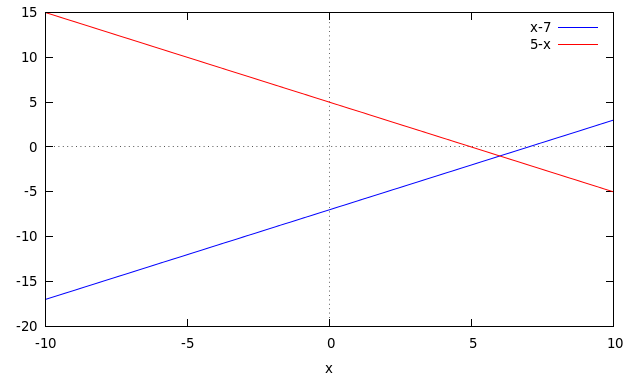
\includegraphics[width=0.6\textwidth]{img/i.png}
\caption{Aufgabe (i)}
\end{figure}

\begin{align}
x - y &= 7 \hspace*{0.3cm}\mycirc{1}\\
x + y &= 5 \hspace*{0.3cm}\mycirc{2}
\end{align}
Wir erhalten:
\begin{equation}
\left.
\begin{aligned}
2x = 12 &\hspace*{0.3cm}\mycirc{3} = \mycirc{1} + \mycirc{2} \\
x = 6 &\hspace*{0.3cm}\mycirc{4} = \mycirc{3} : \mycirc{2} \\
y = -1 &\hspace*{0.3cm}\mycirc{5} = \mycirc{2} - \mycirc{4}
\end{aligned}
\right\}
\quad\text{Das System hat \textbf{genau eine Lösung}.}
\end{equation}
    
\item[(ii)]

\begin{figure}[ht]
\centering
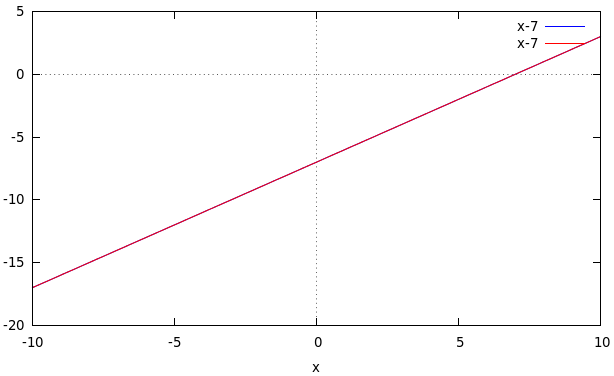
\includegraphics[width=0.6\textwidth]{img/ii.png}
\caption{Aufgabe (ii)}
\end{figure}

\begin{align}
x - y = 7 \hspace*{0.3cm}\mycirc{1}\\
2x - 2y = 14 \hspace*{0.3cm}\mycirc{2}
\end{align}
    
$(0,7)$ ist eine Lösung, auch $(8,1)$ und $(-2,-9)$.
Das System hat \textbf{unendlich viele Lösungen:}
\begin{align}
L = \{\lambda, \lambda-7: \lambda \in \Zb{R}\}
\end{align}
    
\item[(iii)]

\begin{figure}[ht]
\centering
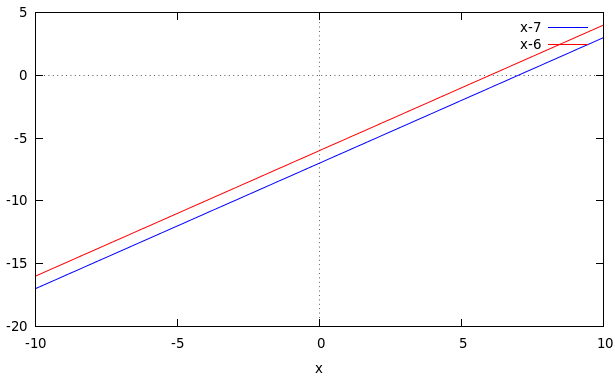
\includegraphics[width=0.6\textwidth]{img/iii.png}
\caption{Aufgabe (iii)}
\end{figure}

\begin{align}
x - y = 7 \hspace*{0.3cm}\mycirc{1}\\
2x - 2y = 12 \hspace*{0.3cm}\mycirc{2}
\end{align}
2 parallele Linien, das System hat \textbf{keine Lösung}.
\end{itemize}

\subsection{(n = 3)}
Der 'Raum'\index{Raum} $\Zb{R}^{3}$ besteht aus allen geordneten Tripeln von reellen Zahlen
\begin{align}
\Zb{R}^{3} := \{(a_1,a_2,a_3):a_1, a_2, a_3 \in \Zb{R}\}
\end{align}
Eine lineare Gleichung in $\Zb{R}^{3}$

\begin{align}
a_1 x_a + a_2 x_2 + a_3 x_3 = b
\end{align}

$x_1, x_2, x_3$: Variablen - $a_1, a_2, a_3, b \in \Zb{R}$
entspricht der Menge

\begin{align}
L := \{(x_1,x_2,x_3) \in \Zb{R}^{3}: a_1 x_1 + a_2 x_2 + a_3 x_3 = 0\}
\end{align}
Falls $a_1=a_2=a_3=0$, ist $L=\Zb{R}^{2}$ für $b=0$ und $L=\emptyset$ für $b \neq 0$. Andernfalls entspricht die
lineare Gleichung einer Ebene in $\Zb{R}^{3}$.

\paragraph{Beispiel}
Betrachten wir für beliebige $\lambda, \mu \in \Zb{R}$.

\begin{align}
x_1 + x_3 = 0 \hspace*{0.3cm}\mycirc{1}\\
x_1 + x_2 + x_3 = 1 \hspace*{0.3cm}\mycirc{2}\\
2x_1 - x_2 + \lambda x_3 = \mu \hspace*{0.3cm}\mycirc{3}
\end{align}
Daraus wird:
\begin{align}
                     x_2 = 1 \hspace*{0.3cm}\mycirc{4} &= \mycirc{2} - \mycirc{1}\\
-x_2 + (\lambda-2) x_3 = \mu \hspace*{0.3cm}\mycirc{5} &= \mycirc{2} - 2\cdot\mycirc{1} \\
   (\lambda-2) x_3 = 1 + \mu \hspace*{0.3cm}\mycirc{6} &= \mycirc{4} + \mycirc{5} 
\end{align}
Falls $\lambda=2$, haben wir keine Lösung für $\lambda \neq -1$ und \textbf{unendlich viele} für $\lambda = -1$.
\begin{align}
L = \{(\alpha, 1, -\alpha): \alpha \in \Zb{R}\}
\end{align}

Andernfalls $(\lambda \neq 2)$ haben wir \textbf{genau eine Lösung}:
\begin{align}
x_1 = \frac{1+\mu}{2-\lambda} \\
x_2 = 1 \\
x_3 = \frac{1+\mu}{\lambda-2}
\end{align}

\subsection{(n beliebig)}
Wir betrachten geordnete n-Tupel von reellen Zahlen
\begin{align}
a = (a_1,...,a_n):a_1, ..., a_n \in \Zb{R}
\end{align}
'geordnet' bedeutet $(a_1,...,a_n) = (a_1',...,a_n') \Rightarrow a_1 = a_1', ... , a_n = a_n'$.
Die Menge aller geordneten n-Tupel von reellen Zahlen
\begin{align}
\Zb{R}^{n} := \{(a_1, ..., a_n) : a_1, ..., a_n \in \Zb{R}\}
\end{align}
heisst der \textbf{reelle Standardraum der Dimension n}.

\paragraph{Bemerkung} Wir können mit n-Tupeln rechnen:
\begin{align}
(a_1, ..., a_n) + (b_1, ..., b_n) := (a_1 + b_1, ..., a_n + b_n)\\
\lambda \cdot (a_1, ..., a_n) := (\lambda a_1, ..., \lambda a_n), \lambda \in \Zb{R}
\end{align}
$\Zb{R}^{n}$ mit den Operationen \textbf{Addition und Multiplikation} mit einer Zahl $\lambda$ ist ein wichtiges
Beispiel eines Vektorraums.

\paragraph{Lineare Gleichungen} Seien $a_1, ..., a_n, b \in \Zb{R}$ und $x_1, ..., x_n$ Variablen. Dann heisst
\begin{align}
a_1 x_1 + \cdots + a_n x_n = b
\end{align}
eine \textbf{lineare Gleichung} in den Variablen $x_1, ..., x_n$.
Falls auch $b=0$, heisst die Gleichung \textbf{homogen}\index{homogen}.\\\\
Ein \textbf{lineares Gleichungssystem} besteht aus $m$ linearen Gleichungen in $n$ Variablen.

\begin{align}
a_{ii} x_{i} + \cdots &+ a_{in} x_n = b_i \\
                      &\vdots \\
a_{mi} x_{i} + \cdots &+ a_{mn} x_n = b_n
\end{align}
Das System heisst homogen, falls $b_1 = \cdots = b_m = 0$.\\
Die \textbf{Lösungsmenge} des Systems besteht aus allen n-Tupeln
$(x_1, \cdots, x_n) \in \Zb{R}^{n}$\textrm{, die alle Gleichungen erfüllen.} \\\
Wie charakterisiert man die \f{Lösung} eines solchen Sysems?
Man kann ein lineares Gleichungssystem mit Hilfe von Matrizen darstellen:
\begin{align}
A x  = b
\end{align}
wobei 
\begin{align}
A := \begin{pmatrix} a_{ii} & \cdots & a_{in} \\ \vdots &  & \vdots \\ a_{mi} & \cdots & a_{mn} \end{pmatrix} \\
x := \begin{pmatrix} x_{1}  \\ \vdots  \\ x_{n} \end{pmatrix} \\
b := \begin{pmatrix} b_{1}  \\ \vdots  \\ b_{m} \end{pmatrix} 
\end{align}

\section{Matrizen}\index{Matrizen}
Seien m, n positive natürliche Zahlen
\begin{align}
 (m, n \in \Zb{N}\setminus\{0\})
\end{align}
Eine \textbf{$m\times n$ Matrix über $\Zb{R}$} mit $m$ Zeilen und $n$ Spalten besteht aus $m \cdot n$ reellen Zahlen
$a_{ij} (r=1\cdots m, j=1\cdots n)$, geschrieben
\begin{align}
A = (a_{ij}) = \begin{pmatrix} a_{ii} & \cdots & a_{in} \\ \vdots &  & \vdots \\ a_{mi} & \cdots & a_{mn} \end{pmatrix}
\end{align}
zum Beispiel
\begin{align}
\begin{pmatrix} 3 & 5 \\ 0 & -1 \end{pmatrix}
\text{ oder } \begin{pmatrix} \pi & -1 \\ 0 &  \frac{5}{2} \\ 1 & 0 \end{pmatrix} 
\end{align}
Die Elemente $a_{ij}$ nennt man \f{Komponenten}\index{Komponenten} der Matrix $A = (a_{ij})$. Zwei Matrizen $A =
(a_{ij})$ und $B = (b_{ij})$ sind \f{gleich}, geschrieben $A=B$, wenn $A$ und $B$ beide $m\times n$-Matrizen sind und
$a_{ij}=b_{ij}$ für alle $i=1\cdots m, j=1\cdots n$ gilt.

\subsection{Rechnen mit Matrizen}
Wir können mit $m\times n$-Matrizen rechnen.\index{Matrizen!rechnen mit}\\
Seien $A = (a_{ij}), B = (b_{ij})$ $m\times n$-Matrizen über $\Zb{R}$ und $\lambda \in \Zb{R}$:
\begin{align}
 A + B = (a_{ij} + b_{ij})
\end{align}
(d.h. $A + B$ ist definiert als $m\times n$-Matrix $(c_ij)$ wobei $c_{ij}=a_{ij}+b_{ij}$ für $i=1\cdots m, j=1\cdots n$).
\begin{align}
 \lambda \cdot A = (\lambda\cdot a_{ij})
\end{align}
Die Menge $Mat(m, n; \Zb{R})$ aller $m\times n$-Matrizen über $\Zb{R}$ mit \f{Addition} und \f{Multiplikation mit einer
Zahl} ist noch ein wichtiges Beispiel eines Vektorraumes.

\subsection{Umformung von Gleichungen zu Matrizen}
Gleichungen $\rightarrow$ Matrizen

\begin{align}
2x_1 + 3x_2 = 5 \\
x_1 - 2x_2 = 0
\end{align}
wird zu
\begin{align}
Ax = b  \\
\Leftrightarrow \begin{pmatrix} 2 & 3 \\ 1 & -2 \end{pmatrix} \begin{pmatrix} x_1 \\ x_2 \end{pmatrix} = \begin{pmatrix} 5 \\ 0 \end{pmatrix}
\end{align}

\paragraph{Anmerkung} Wir können $\Zb{R}^n$ mit $Mat(n, 1; \Zb{R})$ \f{identifizieren}, und die Elemente von $\Zb{R}^n$ \f{Spaltenvektoren}\index{Spaltenvektoren}. Analog heissen die Elemente von $Mat(1,n; \Zb{R})$ \f{Zeilenvektoren}\index{Matrizen!Zeilenvektor}. Wir identifizieren auch eine $1\times 1$-Matrix $(a)(a \in \Zb{R})$ mit $a$.

Wir definieren nun auch
\begin{itemize}
 \item die $m\times n$ \f{Nullmatrix}\index{Nullmatrix} $0^{m\cdot n}$ (oder 0), deren Elemente alle $0$ sind.
 \item das \f{Negative} von $A=(a_{ij}): A := (-a_{ij})$.
\end{itemize}

\begin{lemma}
\label{lemma121}
Seien $A=(a_{ij}), B=(b_{ij}), C=(c_{ij}) \in Mat(m, n; \Zb{R})$.
Dann gilt:
\begin{itemize}
 \item[(i)] $A + B = B + A$ (kommutativ)
 \item[(ii)] $(A + B) + C = A + (B + C)$ (assoziativ)
 \item[(iii)] $A + 0 = A = 0 + A$ (neutrales Element)
 \item[(iv)] $A + (-A) = 0 = (-A) + A$ (inverses Element)
\end{itemize}
\end{lemma} 
\paragraph{Beweis}
Wir betrachten nur $(ii)$. $(i), (iii), (iv)$ sind sehr ähnlich.\\
Seien
\begin{align}
 L = (l_{ij}) := (A+B)+C \\
 R = (r_{ij}) := A + (B + C)
\end{align}
Zu zeigen: $L=R$ für $i=1...m$, $j=1...n$
\begin{align}
 l_{ij} &= (a_{ij}+b_{ij}) + c_{ij}\textrm{ (Definition der Addition)} \\
        &= a_{ij} + (b_{ij} + c_{ij})\textrm{ (rechnen in }\Zb{R}\textrm{)} \\
        &= r_{ij} \textrm{ (per definitionem)  }
\end{align} \hfill $\Box$

\subsection{Matrixmultiplikation}
Wir könnten Matrixmultiplikation durch
\begin{align}
 A \cdot B := (a_{ij}\cdot b_{ij})
\end{align}
definieren, \textit{aber} es gibt eine (kompliziertere!) Definition, welche nützlicher ist.
\paragraph{Beispiel:} Bevölkerungszahlen. \\
Manchester hat 500'000 Einwohner, Liverpool 300'000. Nehmen wir nun an, dass jedes Jahr 5\% der Einwohner nach Liverpool umziehen, und 10\% der Einwohner Liverpools nach Manchester\footnote{Zur Vereinfachung rechnen wir ohne Geburten oder Todesfälle}.

Nach einem Jahr:
\begin{itemize}
 \item Manchester: $(0.95 \cdot 500'000) + (0.1 \cdot 300'000)$ = 505'000 Einwohner
 \item Liverpool: $(0.9\cdot 300'000) + (0.05\cdot 500'000)$ = 295'000 Einwohner
\end{itemize}
Mit Matrizen:
\begin{align}
 \begin{pmatrix}
  0.95 & 0.1\\
  0.05 & 0.9
 \end{pmatrix}
\cdot 
 \begin{pmatrix}
  500'000 \\
  300'000
 \end{pmatrix}
=
 \begin{pmatrix}
  505'000 \\
  295'000
 \end{pmatrix}
\end{align}

\subsection{Komplexere Matrixmultiplikation}\index{Matrizen!Multiplikation}
Zuerst betrachten wir
\begin{itemize}
 \item einen Zeilenvektor $a = (a_i, ..., a_n)$
 \item einen Spaltenvektor $b = \begin{pmatrix}
                                 b_i \\ \vdots \\ b_n
                                \end{pmatrix}$
\end{itemize}
und definieren 
\begin{align}
 a\cdot b = \sum_{i=1}^{n} a_i b_i+...+a_n b_n
\end{align}
\paragraph{Beispiel}
\begin{align}
 (1\,\,\,2\,\,-1)\cdot \begin{pmatrix} 3 \\ -1 \\ 2 \end{pmatrix}
= (1)(3) + (2)(-1) + (-1)(-2) = 3-2+2 = 3
\end{align}

Seien nun
\begin{align}
 A \in Mat(\f{m}, n, \Zb{R}) \\
 B \in Mat(n, \f{p}; \Zb{R})
\end{align}

Wir definieren $A \cdot B := C$ wobei $C = (c_{ij}) \in Mat(m, p; \Zb{R})$ und 
\begin{align}
 c_{ij} := \sum_{k=1}^{n} a_{ik} b_{kj} \Rightarrow \textrm{(Zeilenvektor i von A)} \cdot \textrm{Spaltenvektor j von B}
\end{align}
Wir schreiben oft $AB$ statt $A\cdot B$.

\paragraph{Beispiel}
\begin{align}
 A &= \begin{pmatrix} 1 & 2 & 1 \\ 0 & -3 & -1\end{pmatrix}\in Mat(2,3; \Zb{R}) \\ 
 B &= \begin{pmatrix} -1 & 2 \\ 1 & 0 \\ 1 & 3\end{pmatrix}\in Mat(3,2; \Zb{R}) \\
 AB :&= C = c_{ij} \in Mat(2,2; \Zb{R}) \\
 c_{11} :&= (1 2 1)\cdot \begin{pmatrix} -1 \\ 1 \\ 1 \end{pmatrix} = (1)(-1) + (2)(1) + (1)(1) = 2 \\
 c_{12} :&= (1 2 1)\cdot \begin{pmatrix} 2 \\ 0 \\ 3 \end{pmatrix} = 5 \\
 c_{21} :&= (0 -3 -1)\cdot \begin{pmatrix} -1 \\ 1 \\ 1 \end{pmatrix} = -4 \\
 c_{22} :&= (1 -3 -1)\cdot \begin{pmatrix} 2 \\ 0 \\ 3 \end{pmatrix} = -3 \\
 AB &= C = \begin{pmatrix} 2 & 5 \\ -4 & -3 \end{pmatrix} \\
 BA &= \begin{pmatrix} -1 & .8 & -3 \\ 1 & 2 & 1 \\ 1 & -1 & -2 \end{pmatrix}
\end{align}

\paragraph{Anmerkung:}$AB \neq BA$

\subsection{Quadratische Matrizen}\index{Matrizen!quadratische}
Matrizen in $Mat(n, n; \Zb{R})$ heissen \f{quadratisch}. 
Besondere Beispiele sind die $x\times n$ \f{Einheitsmatrizen}:
\begin{align}
 E^{(n)} := (d_{ij}) = \begin{pmatrix} 1 & 0 & \cdots & 0 \\
				       0 & 1 & \ddots & 0 \\
				       \vdots & \ddots & \ddots & 0 \\
				       0 & \cdots & 0 & 1 \\
\end{pmatrix}\begin{pmatrix} 2 \\ 0 \\ 3 \end{pmatrix}
\end{align}
wobei 
\begin{align}
d_{ij} := \left\{ \begin{matrix} 1 \text{ falls } i=j \\ 0 \text{ andernfalls} \end{matrix}\right.
\end{align}
Für eine quadratische Matrix $A \in Mat(n, n;\Zb{R})$ wird auch die \f{Matrixpotenz} $A^{\lambda}$ wie folgt induktiv definiert:
\begin{align}
 A^{0} := E \\
 A^{k+1} = A^{k} \cdot A, k \in (\Zb{N})
\end{align}

\paragraph{Beispiel}
\begin{align}
 A = \begin{pmatrix} 1 & 2 \\ -1 & 3 \end{pmatrix} \\
 A^0 = \begin{pmatrix} 1 & 0 \\ 0 & 1 \end{pmatrix} \\
 A^1 = \begin{pmatrix} 1 & 2\\ -1 & 3\end{pmatrix}\cdot \begin{pmatrix} 1 & 0 \\ 0 & 1 \end{pmatrix} = \begin{pmatrix} 1 & 2\\ -1 & 3\end{pmatrix} \\
 A^2 = \begin{pmatrix} 1 & 2\\ -1 & 3\end{pmatrix}\cdot \begin{pmatrix} 1 & 2\\ -1 & 3\end{pmatrix} = \begin{pmatrix} -1 & 8 \\ -4 & 7\end{pmatrix}
\end{align}

\begin{lemma}
\label{lemma122}

\begin{itemize}
 \item[(i)] $(AB)C = A(BC)$: Assoziativität für
\begin{align}
 A &\in Mat(m,n; \Zb{R}) \\ 
 B &\in Mat(n,p; \Zb{R}) \\
 C &\in Mat(p,q; \Zb{R}) 
\end{align}

 \item[(ii)] $A(B+C) = AB + AC$ für
\begin{align}
 A &\in Mat(m,n; \Zb{R}) \\ 
 B, C &\in Mat(n,p; \Zb{R})
\end{align}

 \item[(iii)] $(A+B)C = AC + BC$ für 
\begin{align}
 A, B &\in Mat(m,n; \Zb{R}) \\ 
 C &\in Mat(n,p; \Zb{R})
\end{align}

 \item[(iv)] $AE^{(n)} = A$ für $A \in Mat(m,n;\Zb{R})$\\
$E^{(m)}A = A$ für $A \in Mat(m,n;\Zb{R})$

 \item[(v)] $A^i A^j = A^{i+j}$ für
\begin{align}
 A \in Mat(m,n; \Zb{R}), i,j \in \Zb{N} 
\end{align}
\end{itemize}
\end{lemma}

\paragraph{Beweis} Wir beweisen (i) und (v)
\begin{itemize}
 \item[(i)] Seien 
\begin{align}
\left. \begin{array}{cl} L = (l_{ij}) := (AB)C  \\
R = (r_{ij}) := A(BC) \end{array} \right\} \in Mat(m, g; \Zb{R}) \\
F = (f_{ij}) := AB \in Mat(m, p; \Zb{R}) \\
G = (g_{ij}) := AB \in Mat(n, q; \Zb{R}) 
\end{align}
Zu zeigen: $L = R$, d.h. $FC = AG$.
\begin{align}
 l_{ij} &= \sum_{k=1}^{p} f_{ik} c_{kj} \text{ (per definitionem)}\\
        &= \sum_{k=1}^{p} \left( \sum_{s=1}^{n} a_{is} b_{sk} \right) \text{ (per def.)}\\
        &= \sum_{s=1}^{n} a_{is} \left( \sum_{s=1}^{n} b_{sk} c_{kj} \right) \text{ (rechnen in }\Zb{R}\text{)}\\
        &= \sum_{a_{is}}^{g_{sj}} \text{(per def.)}\\
        &= r_{ij} \text{ (per def.)   } 
\end{align}\hfill $\Box$

 \item[(v)] Wir zeigen mit Induktion über j, dass $A^i A^j = A^{i+j}$ für alle $i,j \in \Zb{N}$.
\begin{itemize}
 \item[-] \f{Induktionsanfang:} $j=0$ (zeige, dass Annahme wahr ist)
\begin{align}
A^i A^0 &= A^i E \text{(per def.)} \\
        &= A^i \text{(mit iv)} \\
        &= A^{i+0}
\end{align}
\item[-] \f{Induktionsschritt} von $j$ auf $j+1$. \f{Induktionsannahme:} $A^i A^j = A^{i+j}\text{ für alle } i \in \Zb{N}$.\\
Zu zeigen: $A^i  A^{j+1} = A^{i+j+1}$ für alle $i \in \Zb{N}$.
\begin{align}
 A^i A^{j+1} &= A^i(A^j A) \text{ (per def.)} \\
         &= (A^i A^j)A \text{ (mit i)}\\
         &= A^{i+j} A\text{ (Induktionsannahme)}\\
         &= A^{i+j+1} \text{ (per def.)  }
\end{align} \hfill $\Box$
\end{itemize}
\end{itemize}
% DATE 21.09.

\section{Das Gauss-Eliminationsverfahren}\index{Gauss-Eliminationsverfahren}
\f{Ziel:} Ein Verfahren zum Lösen von linearen Gleichungssystemen.\\
\f{Idee:} Wir benutzen 'elementare Zeilenumformungen' um ein Gleichungssystem auf eine einfache 'Zeilenstufenform' mit denselben Lösungen zu bringen.\\\\
Wir betrachen lineare Gleichungssysteme in der Form:
\begin{align}
 Ax = b
\end{align}
wobei $A \in Mat(m, n; \Zb{R}), x \in \Zb{R}^n, b \in \Zb{R}^n$.\\\\
$A$ heisst \f{Koeffizientenmatrix}\index{Matrizen!Koeffizientenmatrix} und 
\begin{align}
(A, b):= \begin{pmatrix} a_{ii} & \cdots & a_{in} & b_{i} \\ \vdots & & \vdots & \\ a_{mi} & \cdots & a_{mn} & b_{m}\end{pmatrix} 
\end{align}
\f{erweiterte Koeffizientenmatrix}\index{Matrizen!erweiterte Koeffizientenmatrix} des Systems.\\\\
Wir betrachen auch die Lösungsmenge:
\begin{align}
 Loes(A, b) = \{x \in \Zb{R}^n: Ax=b\}
\end{align}
Beobachten Sie nun, dass Systeme mit Koeffizienten wie
\begin{align}
 \begin{pmatrix} 1 & 0 & 2 \\ 0 & 1 & -1 \end{pmatrix},  
 \begin{pmatrix} 0 & 2 & 0 & -1 \\ 0 & 0 & 3 & 1 \\ 0 & 0 & 0 & 0 \end{pmatrix}, 
 \begin{pmatrix} 1 & 0 & -1 & 35 \\ 0 & 0 & 2 & 10 \\ 0 & 0 & 0 & 5 \end{pmatrix}
\end{align}
einfach zu lösen sind.

\paragraph{Beispiel}
\begin{align}
 (A, b) = \begin{pmatrix}[ccc|c] 1 & 0 & 2 & 1 \\ 0 & 1 & -1 & 3 \end{pmatrix}
\end{align}
Das heisst:
\begin{align}
 x_1 + 2x_3 = 1 \\
 x_2 - x_3 = 3
\end{align}
Dann folgt:
\begin{align}
 x_2 = 3 + x_3 \\
 x_1 = 1 - 2 x_3
\end{align}
Lösung: 
\begin{align}
Loes(A, b) = \{ \begin{pmatrix} 1 - 2\lambda \\ 3 + \lambda \\ \lambda \end{pmatrix}: \lambda \in \Zb{R}\} 
\end{align}

% DATE 21.09.
Wir betrachten drei Darstellungen linearer Gleichungssysteme:

\begin{enumerate}
 \item 'Gleichungsform'
\begin{align}
 a_{11} x_1 + \cdots & + a_{1n} x_n = b_i \\
                     & \vdots \\
 a_{m1} x_i + \cdots & + a_{mn} x_n = b_n
\end{align}
\item 'Matrixform'
\begin{align}
 Ax = b
\end{align}
wobei
\begin{align}
A := \begin{pmatrix} a_{11} & \cdots & a_{1n} \\ \vdots &  & \vdots \\ a_{m1} & \cdots & a_{mn} \end{pmatrix} \in Mat(m, n, \Zb{R}) \\
x := \begin{pmatrix} x_{1}  \\ \vdots  \\ x_{n} \end{pmatrix} \\
b := \begin{pmatrix} b_{1}  \\ \vdots  \\ b_{m} \end{pmatrix}.
\end{align}

\item 'Erweiterte-Koeffizientenmatrix-Form'
\begin{align}
(A, b) := \begin{pmatrix}[ccc|c] a_{11} & \cdots & a_{1n} & b_1 \\ \vdots &  & \vdots & \vdots \\ a_{m1} & \cdots & a_{mn} &b_n \end{pmatrix} 
\end{align}
\end{enumerate}

Wir suchen die \f{Lösungsmenge}: 
\begin{align}
 Loes(A,b) = \{ x \in \Zb{R}^n: Ax = b\} \\
 A=(a_{ij}) \in Mat(m, n, \Zb{R})
\end{align}
heisst in \f{Zeilenstufenform}\index{Zeilenstufenform}, wenn sie von der folgenden Form ist:
\begin{align}
A = \begin{pmatrix} j_0 & j_1 & j_2 & \cdots & j_r \\ 0 & \ast & & & \\ 0 & 0 & \ast & & \\ 0 & 0 & 0 &\ddots & x \end{pmatrix}
\end{align}
wobei $\ast$ 'ungleich Null' bedeutet.

\paragraph{Beispiel}
\begin{align}
 \begin{pmatrix}
  0 & 2 & 5 & 1 & 0 \\
  0 & 0 & -1 & 0 & -1 \\
  0 & 0 & 0 & 0 & 0
 \end{pmatrix},
 \begin{pmatrix}
  -1 & 2 & -1 \\
  0 & 0 & 3  \\
  0 & 0 & 0 \\
  0 & 0 & 0
 \end{pmatrix}
\end{align}

Präziser formuliert: $A$ ist in \f{Zeilenstufenform} falls:
\begin{itemize}
 \item[(1)] Es gibt $r \in \{0 ,1, \cdots, m\}$, so dass in den Zeilen $1 \cdots r$ nicht nur Nullen stehen, und in den Zeilen $r+1, \cdots, m$ nur Nullen stehen.
 \item[(2)] $j_1 < j_2 < \cdots < j_r$ wobei für $i=1\cdots r$ gilt: $j_i := min\{j: a_{ij} \neq 0\}$
\end{itemize}

\f{Anmerkung:} Durch eine Umordnung der Spalten von $A$\footnote{d.h., eine andere Numerierung der Variablen des entsprechenden Gleichungssystems} kann man immer annehmen:

\begin{align}
 j_1 = 1, \cdots, j_r = r
\end{align}

\f{Beispiel}
\begin{align}
x_1 + 2 x_2 - x_3 + x_4 = 1 \\
2x_3 - x_4 = 0 \\
\begin{pmatrix}[cccc|c]
1 & 2 & -1 & 1 & 1 \\
0 & 0 & 2 & -1 & 0
\end{pmatrix}
\end{align}
können wir umformulieren als
\begin{align}
y_1 - y_2 + 2y_3 + y_4 = 4 \\
2y_2 -y_4 = 0 \\
\begin{pmatrix}
1 & -1 & 2 & 1 & 1 \\
0 & 2 & 0 & -1 & 0
\end{pmatrix}
\end{align}
Das ergibt
\begin{align}
y_1=x_1, y_2=x_3, y_3 = x_2, y_4 = x_4
\end{align}

Betrachten Sie nun ein System:
\begin{align}
 (A,b) = \left. \begin{pmatrix}[cccc|c]
          a_{11} & & & & b_1\\
           & a_{22} & & & b_2\\
           & & \ddots & & \vdots \\
           & & & a_{rr} & b_{r}\\
           & & & & b_{r+1} \\
           & & & & \vdots\\
           & & & & b_m
         \end{pmatrix}
	 \right\} m
\end{align}

Falls $b_i = 0$ für $i \in \{r+1, \cdots, m\}$, dann ist $Loes(A, b) = \emptyset$. Andernfalls
\begin{itemize}
 \item $b_{r+1} = \cdots = b_m = 0$
 \item $x_{r+1}, \cdots, x_n$ heissen \f{freie Variablen}\index{Variablen!gebundene} 
 \item $x_{1}, \cdots, x_r$ heissen \f{gebundene Variablen}\index{Variablen!freie}
\end{itemize}
Man setzt
\begin{align}
k := n-r
\end{align}
und wählt 
\begin{align}
\lambda_1, ..., \lambda_k \text{ als Parameter mit } x_{r+1} = \lambda_1, ...,  x_n = \lambda_k 
\end{align}
Zur Berechnung der $x_1, \cdots, x_r$ beginnt man mit 
\begin{align}
 a_{rr} x_r + a_{r, r+1} \lambda_1 + \cdots + a_{r n} \lambda_k = b_r 
\end{align}
und erhält
\begin{align}
x_r = \frac{1}{a_{rr}}(b_r - a_{r,r+1} \lambda_1 - \cdots - a_{r n} \lambda_k)
\end{align}
Dann berechnet man ähnlicherweise $x_{r-1}, \cdots, x_1$.

\f{Anmerkung}
Falls $n=r$ so ($k=0$), dann haben wir keinen Parameter und \f{genau eine Lösung}. Andernfalls erhalten wir unendlich viele Lösungen.

\f{Beispiele}
\begin{itemize}
 \item[(i)] 
\begin{align}
 (A, b) =
\begin{pmatrix}[ccc|c]
1 & 0 & 1 & 1  \\
0 & 2 & -1 & 1 \\
0 & 0 & 0 & 1 
\end{pmatrix} \\
Loes(A, b) = \emptyset
\end{align}

 \item[(ii)]
\begin{align}
\begin{pmatrix}[ccc|c]
1 & 0 & 1 & 1  \\
0 & 2 & -1 & 0 \\
0 & 0 & 0 & 1 
\end{pmatrix}
,
\begin{pmatrix}
x_1 \\
x_2 \\
x_3  
\end{pmatrix} =
\begin{pmatrix}
0 \\
\frac{1}{2} \\
1
\end{pmatrix} \\
Loes(A, b) = 
\begin{pmatrix}
0 \\
\frac{1}{2} \\
1
\end{pmatrix}
\end{align}

\item[(iii)]
\begin{align}
(A, b) = \begin{pmatrix}[cccccc|c]
3 & 1 & 1 & 0 & 0 & 0 & 2 \\
0 & -1 & 1 & 0 & 2 & 1 & 3 \\
0 & 0 & 2 & 1 & 1 & -3 & 4 \\
0 & 0 & 0 & 1 & -1 & -1 & 0 \\
0 & 0 & 0 & 0 & 0 & 0 & 0 
\end{pmatrix} \\
m = 5, n = 6, r = 4
\end{align}

$\lambda_1 = x_5, \lambda_2 = x_6$. Weitere Umformungen:
\begin{itemize}
\item Schritt 1:
\begin{align}
 x_4 - \lambda_1 - \lambda_2 = 0 \\
 \Rightarrow x_4 = \lambda_1 + \lambda_2
\end{align}

\item Schritt 2:
\begin{align}
 2x_3 + (\lambda_1 + \lambda_2) + \lambda_1 - 3\lambda_2 = 4 \\
 \Rightarrow x_3 = 2 - \lambda_1 + \lambda_2
\end{align}

\item Schritt 3:
\begin{align}
 -x_2 + (2 - \lambda_1 + 2\lambda_2) + 2\lambda_1 + \lambda_2 = 3 \\
 \Rightarrow x_2 = \lambda_1 + 2\lambda_2-1
\end{align}

\item Schritt 4:
\begin{align}
 3x_1 + (\lambda_1 + 2\lambda_2  - 1) + (2- \lambda_1 + \lambda_2) = 2 \\
 \Rightarrow x_1 = \frac{1}{3} - \lambda_2
\end{align}
\end{itemize}
Da die Lösung zwei Parameter beinhaltet, ist die Lösungsmenge unendlich. Spezfifizieren kann man sie wie folgt:
\begin{align}
 Loes(A,b) = \{ \begin{pmatrix}
                 \frac{1}{3} - \lambda_2 \\ \lambda_1 + 2\lambda_2-1 \\ \lambda_1 + \lambda_2 \\ \lambda_1 \\ \lambda_2
                \end{pmatrix}
: \lambda_1, \lambda_2 \in \Zb{R}\}
\end{align}
\end{itemize}

\subsection{Elementare Zeilenumformungen}\index{elementare Zeilenumformungen}
Wir versuchen nun ein beliebiges System auf Zeilenstufenform zu bringen. Dazu benützen wir zwei Typen von \f{elementaren Zeilenumformungen} der erweiterten Koeffizientenmatrix:
\begin{itemize}
 \item[\f{Typ I}] Vertauschung zweier Zeilen
 \item[\f{Typ II}] Addition der $\lambda$-fachen Zeile $i$ mit Zeile $j$, wobei $0 \neq \lambda \in \Zb{R}$ und $i \neq j$
\end{itemize}

\paragraph{Beispiel}
\begin{align}
 (A | b) = 
\begin{pmatrix}[cccc|c]
 0 & 2 & -3 & -1 & 1 \\
 -1 & 2 & 0 & -1 & 0 \\
 2 & 0 & -5 & 2 & -2
\end{pmatrix} \\
I: Z_1 \Leftrightarrow Z_2 \\
\begin{pmatrix}[cccc|c]
 -1 & 2 & 0 & -1 & 0 \\
 0 & 2 & -3 & -1 & 1 \\
 2 & 0 & -5 & 2 & -2
\end{pmatrix} \\
II: Z_3 \rightarrow Z_3 + 2Z_1 \\
\begin{pmatrix}[cccc|c]
 -1 & 2 & 0 & -1 & 0 \\
 0 & 2 & -3 & -1 & 1 \\
 0 & 4 & -5 & 0 & -2
\end{pmatrix} \\
II: Z_3 \rightarrow Z_3 - 2Z_2 \\
\begin{pmatrix}[cccc|c]
 -1 & 2 & 0 & -1 & 0 \\
 0 & 2 & -3 & -1 & 1 \\
 0 & 0 & 1 & 2 & -4
\end{pmatrix} \\
= (\bar{A},\bar{b})
\end{align}

Entscheidend ist nun
\begin{align}
 Loes(A, b) \stackrel{?}{=} Loes(\bar{A}, \bar{b})
\end{align}

\begin{lemma}
 \label{lemma131}
Sei $(\bar{A}, \bar{b})$ durch endlich viele Zeilenumformungen entstanden. Dann gilt:
\begin{align}
 Loes(A, b) = Loes(\bar{A}, \bar{b}) 
\end{align}
\end{lemma}

\paragraph{Beweis}
Es genügt zu zeigen, dass die Lösungen  bei \f{einer} elementaren Zeilenumformung unverändert bleibt.
\begin{itemize}
 \item[\f{Typ I}] Trivial (wir lösen dieselben Gleichungen)
 \item[\f{Typ II}] $(\bar{A}, \bar{b})$ ist $(A, b)$ ausser Zeile $j$.
\begin{align}
 (a_{j1} + \lambda a_{i1}) x_1 + \cdots + (a_{jn}+ \lambda a_{in}) x_n = b_j + \lambda b_i \hspace*{0.5cm} \mycirc{1}
\end{align}
Zu zeigen: $Loes(A, b) = Loes (\bar{A}, \bar{b})$. Oft einfach zu zeigen: Beides sind Teilmengen voneinander. Dies wird im folgenden bewiesen.
\begin{itemize}
\item \f{$Loes(A, b) \subseteq Loes (\bar{A}, \bar{b})$} Sei $x \in Loes(A,b)$. Dann gilt:
\begin{align}
 a_{i1} x_1 + \cdots + a_{in} x_n = b_i \hspace*{0.5cm} \mycirc{2}\\
 a_{j1} x_1 + \cdots + a_{jn} x_1 = b_j \hspace*{0.5cm} \mycirc{3}
\end{align}
Also gilt für $0 \neq \lambda \in \Zb{R}$:
\begin{align}
 \lambda a_{i1} x_1 + \cdots + \lambda a_{in} x_n = \lambda b_i \hspace*{0.2cm} \mycirc{4} \hspace*{0,3cm}\text{ mit } \mycirc{2}
\end{align}
und auch $\mycirc{1}$ (mit $\mycirc{3}$ und $\mycirc{4}$). Deshalb $x \in Loes(\bar{A}, \bar{b})$

\item \f{$Loes(\bar{A}, \bar{b}) = Loes (A, b)$} Ähnlich (Übung). \hfill $\Box$
\end{itemize}
\end{itemize}

\begin{lemma}\f{(Korrektheitsbeweis)}\\
 \label{lemma132}
 Sei $(A, b)$ ein lineares Gleichungssystem mit $A \in Mat(m, n; \Zb{R})$. Dann existiert $(\bar{A}, \bar{b})$, wobei
\begin{itemize}
 \item $(\bar{A}, \bar{b})$ entsteht aus $(A, b)$ durch endlich viele elementare Zeilenumformungen.
 \item $A$ ist in Zeilenstufenform.
\end{itemize}
\end{lemma}
\paragraph{Beweis} Induktion über $m$.
\begin{itemize}
 \item \f{Induktionsanfang}: $m=1$. Dann ist $(\bar{A}, \bar{b})=(A, b)$.
 \item \f{Induktionsschritt}: von $m$ auf $m+1$. \f{Induktionsannahme:} Die Behauptung gilt für alle $n \in \Zb{N}\setminus\{0\}, A \in Mat(m, n; \Zb{R}) und b \in \Zb{R}^m$
 \item \f{Zu zeigen:} Die Behauptung gilt für alle $n \in \Zb{N}\setminus\{0\}, A \in Mat(m+1, n; \Zb{R}) und b \in \Zb{R}^m$. \\
  Falls $A=0$, dann ist $(\bar{A}, \bar{b})=(A, b)$. Andernfalls betrachten wir die kleinste Zahl $j \in \{1, ..., n\}$ mit $a_{ij} \neq 0$ für ein $i \in \{1, ..., m\}$. \\
  Dann entsteht durch 0 oder 1 Zeilenumformungen vom Typ I eine Matrix der Form:
\begin{align}
 \begin{pmatrix}[ccccc|c]
  0 & 0 & a_{ij} & \cdots & a_{in} & b_i \\
  \vdots & \vdots & & & & \vdots \\
  0 & 0 & & & &
 \end{pmatrix}
\end{align}
Durch Umformungen vom Typ II macht man alle unterhalb von $a_{ij}$ stehende Komponenten 0:
\begin{align}
 \begin{pmatrix}[ccccc|c]
  0 & 0 & a_{ij} & \cdots & a_{in} & b_i \\
  \vdots & \vdots & 0 & & & \vdots \\
  0 & 0 & \vdots & & & \\
  0 & 0 & 0 & & & \\
 \end{pmatrix}
\end{align}
Mit der Induktionsannahme (denn $A \in Mat(m, k, \Zb{R})$) für ein $k \in \Zb{N}\setminus\{0\}$ erhalten wir
\begin{align}
 \begin{pmatrix}[ccccc|c]
  0 & 0 & a_{ij} & \cdots & a_{in} & b_i \\
  \vdots & \vdots & 0 & b & & \vdots \\
  0 & 0 & \vdots & 0 & c & \\
  0 & 0 & 0 & \vdots & 0 & \\
  0 & 0 & 0 & 0 & \vdots &
 \end{pmatrix}
\end{align} \hfill $\Box$
\end{itemize}

\subsection{Zusammenfassung}
Das \f{Gauss-Eliminationsverfahren}\index{Gauss-Eliminationsverfahren} besteht aus zwei Schritten:
\begin{itemize}
 \item Durch elementare Zeilenumformungen erhält man $(\bar{A}, \bar{b})$, wobei $\bar{A}$ in Zeilenstufenform ist und $Loes(A, b) = Loes(\bar{A}, \bar{b})$
 \item Man berechnet direkt $Loes(\bar{A}, \bar{b})$.
\end{itemize}

\paragraph{Beispiel}
Bestimmen Sie, für welches $\lambda \in \Zb{R}$ das folgende Gleichungssystem lösbar ist und geben Sie gegebenenfalls die Lösung an.
\begin{align}
(A, b) =
\begin{pmatrix}[cccc|c]
  2 & -1 & 1 & -3 & 0\\
  -4 & 2 & -3 & 5 & 1+\lambda \\
 0 & 1 & -2 & 4 & 2\lambda \\
 6 & -2 & 2 & -4 & 1
\end{pmatrix}
\end{align}
Lösungsschritte: $Z_2 \rightarrow Z_2 + 2Z_1$, $Z_4 \rightarrow Z_4 - 3 Z_1$
\begin{align}
\begin{pmatrix}[cccc|c]
  2 & -1 & 1 & -3 & 0\\
  0 & 0 & -1 & -1 & 1+\lambda \\
 0 & 1 & -2 & 4 & 2\lambda \\
 0 & 1 & -1 & 5 & 1
\end{pmatrix}
\end{align}
Danach: $Z_2 \Leftrightarrow Z_3$
\begin{align}
\begin{pmatrix}[cccc|c]
 2 & -1 & 1 & -3 & 0\\
 0 & 1 & -2 & 4 & 2\lambda \\
 0 & 0 & -1 & -1 & 1+\lambda \\
 0 & 1 & -1 & 5 & 1
\end{pmatrix}
\end{align}
$Z_4 \rightarrow Z_4-Z_2$
\begin{align}
\begin{pmatrix}[cccc|c]
 2 & -1 & 1 & -3 & 0\\
 0 & 1 & -2 & 4 & 2\lambda \\
 0 & 0 & -1 & -1 & 1+\lambda \\
 0 & 0 & 1 & 1 & 1-2\lambda
\end{pmatrix}
\end{align}
$Z_4 \rightarrow Z_4 + Z_3$
\begin{align}
\begin{pmatrix}[cccc|c]
 2 & -1 & 1 & -3 & 0\\
 0 & 1 & -2 & 4 & 2\lambda \\
 0 & 0 & -1 & -1 & 1+\lambda \\
 0 & 0 & 0 & 0 & 2-\lambda
\end{pmatrix}=(\bar{A}, \bar{b}) \\ 
\text{ mit } Loes(A, b)=Loes(\bar{A}, \bar{b})
\end{align}
Falls $\lambda \neq 2$, dann ist
\begin{align}
 Loes(A, b) = \emptyset
\end{align}
Andernfalls, $\lambda = 2$ und wir setzen $\mu=x_4$.
Wir erhalten:
\begin{enumerate}
 \item $-x_3-\mu = 3 \Rightarrow x_3 = -3 -\mu$
 \item $x_2 - 2(-3-\mu) + 4 \mu = 4$ \\ $\Rightarrow x_2 = -2 -6\mu$
 \item $2x_1-(-2-6\mu) + (-3-\mu) - 3\mu = 0$ \\ $\Rightarrow 2x_1 = 1-2\mu$ \\ $\Rightarrow x_1 = \frac{1}{2}-\mu$
\end{enumerate}
\begin{align}
Loes(A, b) = \{
\begin{pmatrix}
 \frac{1}{2}-\mu \\
 -2-6\mu \\
 -3-\mu \\
 \mu 
\end{pmatrix}, \mu \in \Zb{R}\} 
\end{align}
Was jetzt? Betrachten Sie eine homogene lineare Gleichung
\begin{align}
 2x + y = 0
\end{align}
$x$ und $y$ 'müssen nicht' reelle Zahlen sein, z.B.
\begin{align}
x = \begin{pmatrix}
 1 \\
 -1 
\end{pmatrix}, y = \begin{pmatrix}
 -1 \\
 2 
\end{pmatrix} \\
x = 2z^2-z, y=-4z^2+2z
\end{align}
Wir fragen:
\begin{itemize}
 \item Woher kommen $x, y$ usw?
 \item Was bedeutet $+$?
\end{itemize}
Wir geben \f{abstrakte} Antworten.

\chapter{Gruppen, Ringe, Körper}\index{Körper}\index{Ring}\index{Gruppe}
Mengen mit Verknüpfungen - sogenannte \f{algebraische Strukturen} - spielen eine wichtige Rolle in der Mathematik.
Zum Beispiel:
\begin{itemize}
 \item $\Zb{N}$ mit $+, -, \cdot, 0, 1$
 \item $\Zb{R}^n$ mit $+$
 \item $Mat(m, n)$ mit $+, 0^{m, n}$
 \item $Mat(n, n)$ mit $\cdot$
 \item $\Zb{N}$ mit 'min' und 'max'
 \item $P(A) = \{B: B \subseteq A\}$, die Potenzmenge von einer Menge $A$, mit $\cap$ und $\cup$.
\end{itemize}
Wir betrachen \f{Klassen} von Strukturen mit gewissen Eigenschaften. Insbesondere: Gruppen, Ringe, Körper, Vektorräume.
\subsection{Mengen und Verknüpfungen}
Seien $A_1, \cdots, A_n, B$ Mengen. Eine Abbildung 
\begin{align}
 a:\{1, \cdots, n\} \rightarrow A_1, \cup \cdots \cup A_n
\end{align}
mit $a(i) \in A$;
heisst ein \f{geordnetes n-Tupel}\index{geordnete n-Tupel}, geschrieben
\begin{align}
 (a_1, \cdots, a_n)
\end{align}
Die Menge aller geordneten n-Tupel von $A_1, \cdots, A_n$ heisst das \f{Direktprodukt}.
\begin{align}
A_1\times \cdots \times A_n := \{(a_1, \cdots, a_n): a_i \in A_i, i=1 \cdots n\}
\end{align}
Falls $A_1 = \cdots = A_n = A$, schreiben wir 
\begin{align}
 A^n = A \times \cdots \times A
\end{align}
Eine Abbildung 
\begin{align}
 f: A_1 \times \cdots \times A_n \rightarrow B
\end{align}
geschrieben auch
\begin{align}
 (a_1, \cdots, a_n) \mapsto f(a_1, \cdots, a_n)
\end{align}
heisst eine \f{n-stellige Verknüpfung}.\index{Verknüpfung!n-stellig}

\section{Gruppen}
Eine Menge $G$ zusammen mit einer zweistelligen (oder \f{binären}) Verknüpfung
\begin{align}
 *: G \times G \rightarrow G \\
 (a, b) \mapsto *(a,b)
\end{align}
heisst ein \f{Gruppoid}.\index{Gruppoid}

\paragraph{Anmerkung}
Wir schreiben '$G$' für die Menge $G$ und auch Gruppoid $G$ mit *. Wir schreiben oft $a*b$ statt $*(a, b)$.

Ein Gruppoid $G$ heisst:
\begin{itemize}
 \item \f{assoziativ} falls $a*(b*c) = (a*b)*c$ für alle $a, b, c \in G$
 \item \f{kommutativ} falls $a*b=b*a$ für alle $a, b \in G$
 \item \f{idempotent}\index{idempotent} falls $a*a=a$ für alle $a \in G$
\end{itemize}
Ein assoziatives Gruppoid heisst eine \f{Halbgruppe}\index{Halbgruppe} und eine idempotente kommutative Halbgruppe heisst \f{Halbverband}\index{Halbverband}. 

\paragraph{Beispiele}
\begin{itemize}
 \item[(i)] $G = \Zb{N}, \Zb{Z}, \Zb{Q}$ oder $\Zb{R}$ mit $a*b := a+b$ oder $a*b := a \cdot b$ ist eine kommutative Halbgruppe\index{Halbgruppe}.
 \item[(ii)] $G = \Zb{N}, \Zb{Z}, \Zb{Q}$ oder $\Zb{R}$ mit $a*b := min(a, b)$ oder $a*b := max(a, b)$ ist ein Halbverband\index{Halbverband}.
 \item[(iii)] $G = \Zb{Q}$ oder $\Zb{R}$ mit dem arithmetischen Mittel: $a*b := \frac{a+b}{2}$ ist ein kommutatives idempotentes (nicht assoziatives) Gruppoid\index{Gruppoid}.
 \item[(iv)] $G = P(A)$ ($A$ eine Menge) mit $a*b := a \cup b$ oder $a*b := a \cap b$ ist
ein Halbverband\index{Halbverband}.
 \item[(iv)] $G = \cup A^n$ (A eine Menge) mit $n \in \Zb{N}$, die Menge aller endlichen Sequenzen ($a_1, \cdots, a_n$) für $a_1, \cdots, a_n \in A$, mit $(a_1, \cdots, a_n)*(b_1, \cdots, b_m) = (a_1, \cdots, a_n, b_1, \cdots, b_m)$ (Konkatenation)ist eine Halbgruppe\index{Halbgruppe}.
\end{itemize}
Eine Halbgruppe $G$ heisst \f{Gruppe}\index{Gruppe} falls:
\begin{itemize}
 \item[(1)] Es gibt ein \f{neutrales Element} $e \in G$, wobei $a*e = a = e*a$ für alle $a \in G$.
 \item[(2)] Zu jedem Element $a \in G$ gibt es ein \f{inverses Element} $a \in G$, wobei $a*a' = e = a' * a$ für alle $a \in G$.
\end{itemize}
Eine kommutative Gruppe heisst abelsch.\index{abelsch!abelsche Gruppe}

\paragraph{Beispiele}
\begin{itemize}
 \item[(i)] $G = \Zb{Z}, \Zb{Q}$ oder $\Zb{R}$ mit $a * b := a + b$ ist eine Gruppe mit neutralem Element $0$ und inversem Element $-a$ für $a$. 
 \item[(ii)] $G = \Zb{Q}\setminus\{0\}$ oder $\Zb{R}\setminus\{0\}$ mit $a*b := a\cdot b$ ist eine Gruppe mit neutralem Element $1$ und inversem Element $\frac{1}{a}$ für a.
\item[(iii)] $G = Mat(m, n; \Zb{R})$ mit $A * B := A + B$ ist eine Gruppe mit $0^{m, n}$ und $-A$.
\item[(iv)] $G = D_n$, die Isometriegruppe\index{Isometriegruppe} eines regelmässigen Polygons in der Ebene, hat $2n$ Elemente ($n$ Drehungen und $n$ Spiegelungen). Die Verknüpfung $*$ ist gegeben durch die Hintereinanderausführung von Symmetrietransformationen.
z.B. in $D_4$ gibt es 4 Drehungen und 4 Spiegelungen.
\end{itemize}

\begin{lemma}
\label{lemma211}
 Sei $G$ eine Gruppe. Dann gilt 
\begin{itemize}
 \item[(i)] Das neutrale Element $e \in G$ ist \f{eindeutig bestimmt}, d.h. $e_1$ und $e_2$ sind neutrale Elemente $\Rightarrow e_1 = e_2$
 \item[(ii)] Das inverse Element $a'$ is für jedes $a\in G$ eindeutig bestimmt, d.h. $b$ und $c$ sind inverse Elemente für $a$.$\Rightarrow b=c$. Deshalb können wir $a^{-1}$ statt $a'$ schreiben.
\end{itemize}
\end{lemma}

\paragraph{Beweis} 
\begin{itemize}
 \item[(i)]
Seien $e_1 \in G$ und $e_2 \in G$ neutrale Elemente. Dann gilt
\begin{align}
  e_1 e_2 = e_1 \\
  \Rightarrow e_1 e_2 = e_2
\end{align}
also $e_1 = e_2$.

\item[(ii)] Seien $b \in G$ und $c \in G$ inverse Elemente für $a \in G$. Dann gilt:
\begin{align}
 b &= be \\
   &= b(ac) \\
   &= (ba)c \\
   &= ec \\
   &= c
\end{align}
\end{itemize}
% DATE 03.10.
Zur Erinnerung: Eine Menge $G$ zusammen mit einer binären Verknüpfung $*: G^2 \rightarrow G$ heisst \f{Gruppe}, falls gilt:
\begin{itemize}
 \item * ist \f{assoziativ}, d.h. $a*(b*c) = (a*b)*c$ füür alle $a, b, c \in G$.
 \item Es gibt ein (eindeutig definiertes) \f{neutrales Element} $e$ mit $a*e=a=e*a$ für alle $a \in G$.
 \item Zu jedem $a \in G$ gibt es ein (eindeutig besimmtes) \f{inverses Element} $a' \in G$ mit $a*a'= e = a' * a$ (Wir schreiben $a^{-1}$ statt a').
\end{itemize}

z.B. $\Zb{Z}$ mit $+$, $\Zb{Q}\setminus\{0\}$ mit $\cdot$, $Mat(m, n; \Zb{R}$ mit $+$, usw.

\paragraph{Wichtige Beispiele:} \f{Permutationsgruppen/Symmetrische Gruppen}\index{Gruppe!Permutationsgruppe}. Seien $A, B, C, D$ Mengen. Dann bezeichnen wir mit Abb $A, B$ die \f{Menge aller Abbildungen} $f: A \rightarrow B$ von $A$ nach $B$.

Sind  $f: A \rightarrow B \in$ Abb $A,B$ und $g: B \rightarrow C \in$ Abb $B,C$, so heisst die Abbildung 
\begin{align}
 g \circ f: A \rightarrow C, x \mapsto g(f(x)) \\
 \textrm{d.h. }(g \circ f)(x) := g(f(x))
\end{align}
 die \f{Komposition} von $f$ und $g$.

Für Abbildungen $f: A \rightarrow B, g: B \rightarrow C, h: C \rightarrow D$:

\begin{align}
 ((h \circ g) \circ f)(x) &= (h \circ g)(f(x)) \\
                                &= h(g(f(x)))
                                &= h((g \circ f)(x))
                                &= (h \circ (g \circ f))(x)
\Rightarrow (h \circ g) \circ f = h \circ (g \circ f)
\end{align}
Also ist Abb $A, A$ mit Komposition eine \f{Halbgruppe}. Ist Abb $A,A$ eine Gruppe?

\paragraph{Die identische Abbildung}
\begin{align}
 id_{A\rightarrow A}, x\mapsto x
\end{align}
ist ein neutrales Element für Abb $A,A$. Aber für $f: A \rightarrow A$ gibt es $g: A \rightarrow A$ mit
\begin{align}
 f \circ g(id_{A}) = g \circ f
\end{align}
genau dann wenn $f$ \f{bijektiv} ist (Aufgabe). Also ist Abb $A, A$ im Allgemeinen keine Gruppe.
Wir betrachen statt 
\begin{align}
 S(A) := \{f \in \text{Abb }A,A: f \textrm{ bijektiv}\}
\end{align}
die symmetrische Gruppe der Menge $A$.\\\\
Falls $A=\{1 \cdot n\}$, schreibt man 
\begin{align}
 S_n \textrm{ statt } S(A)
\end{align}
und nennt $S_n$ \f{Permutationsgruppe}\index{Permutationsgruppe}.

\paragraph{Beispiel} $A=\{1, 2, 3\}$. $S(A) = S_3$ hat 6 Elemente:
\begin{align}
\begin{bmatrix} 1 \longrightarrow 1 \\ 2 \longrightarrow 2 \\ 3 \longrightarrow 3 \\ () \end{bmatrix}
\begin{bmatrix} 1 \longrightarrow 1 \\ 2 \longrightarrow 3 \\ 3 \longrightarrow 2 \\ (2 3) \end{bmatrix}
\begin{bmatrix} 1 \longrightarrow 2 \\ 2 \longrightarrow 1 \\ 3 \longrightarrow 3 \\ (1 2) \end{bmatrix} \\
\begin{bmatrix} 1 \longrightarrow 2 \\ 2 \longrightarrow 3 \\ 3 \longrightarrow 1 \\ (1 2 3) \end{bmatrix}
\begin{bmatrix} 1 \longrightarrow 3 \\ 2 \longrightarrow 1 \\ 3 \longrightarrow 2 \\ (1 3 2) \end{bmatrix}
\begin{bmatrix} 1 \longrightarrow 3 \\ 2 \longrightarrow 2 \\ 3 \longrightarrow 1 \\ (1 3) \end{bmatrix}
\end{align}
\f{Anmerkung} $S_n$ hat $n! = 1 \times 2 \times \cdots \times n$ Elemente.
\begin{align}
 (1 2 3)(1 2) = (1 3) \\
 (1 2)(1 2 3) = (2 3)
\end{align}
Also ist $S_3$ nicht \f{abelsch}\index{abelsch}.

\begin{lemma}
\label{lemma212}
 Sei $G$ eine Gruppe und $a, b, c \in G$. Dann gilt:
\begin{itemize}
 \item[(i)] $(a^{-1})^{-1} = a$
 \item[(ii)] $(ab)^{-1} = b^{-1}a^{-1}$
 \item[(iii)] $ab = ac \Rightarrow b=c$
 \item[(iv)] $ba = ca \Rightarrow b=c$
\end{itemize}
\end{lemma}
\paragraph{Beweis}
\begin{itemize}
 \item[(i)] Bemerken Sie, dass
\begin{align}
 aa^{-1} = e = a^{-1}a
\end{align}
Also ist $a$ das inverse Element für $a^{-1}$ und nach Lemma \ref{lemma211} folgt
\begin{align}
 (a^{-1})^{-1} = a
\end{align}
\item[(ii)] Ähnlicherweise:
\begin{align}
 (b^{-1}a^{-1})(ab) &= b^{-1}(a^{-1}a)b\\
                    &= b^{-1}eb \\
                    &= b^{-1}b \\
                    &= e
\end{align}
und $(ab)(b^{-1}a^{-1}) = e$, so
\begin{align}
 (ab)^{-1} = b^{-1}a^{-1}
\end{align}

\item[(iii)]
\begin{align}
ab = ac &\Rightarrow a^{-1}(ab) = a^{-1}(ac) \\
        &\Rightarrow (a^{-1}a)b = (a^{-1}a)c \\
        &\Rightarrow eb = ec
        &\Rightarrow b = c
\end{align}

\item[(iv)] Analog. \hfill $\Box$
\end{itemize}
Es gibt eine nützliche äquivalente Charakterisierung von Gruppen. Betrachen Sie für ein Gruppoid $G$ und $a \in G$ die Abbildungen:
\begin{align}
 \tau_a : G \rightarrow G, x \mapsto x*a \\
 a^{\tau}: G \rightarrow G, x \mapsto a*x
\end{align}

\begin{lemma}
\label{lemma213}
 Sei $G$ eine nichtleere Halbgruppe. Dann sind die folgenden Aussagen äquivalent:
\begin{itemize}
 \item[(1)] $G$ ist eine Gruppe.
 \item[(2)] $\tau_a$ und $a^{\tau}$ sind bijektiv.
\end{itemize}
\end{lemma}
\paragraph{Beweis}

\begin{itemize}
\item[$(1)\Rightarrow(2)$] Sei $G$ eine Gruppe und $a \in G$.
\begin{itemize}
 \item $\tau_a$ ist injektiv, denn für $b, c \in G$
\begin{align}
\tau_a(b) &= \tau_a(c) \\
\Rightarrow ba &= ca \\
\Rightarrow b &= c
\end{align}
\item $\tau_a$ ist surjektiv, denn für $b \in G$
\begin{align}
 \tau_a(ba^{-1}) &= ba^{-1}a \\
                 &= be \\
                 &= b
\end{align}
$a_{\tau}$ ist sehr ähnlich.
\end{itemize}

\item[$(2)\Rightarrow(1)$] Seien $\tau_a$ und $a_{\tau}$ bijektiv für alle $a \in G \neq \emptyset$.
Wir haben ein $a \in G$. Dann 
\begin{align}
 e_1a = a
\end{align}
für ein $e_1\in G$ ($\tau_a$ ist surjektiv).
Betrachen Sie nun $x \in G$. Dann $ab = x$ für ein $b \in G$ ($a^{\tau}$ ist surjektiv).
Also folgt
\begin{align}
 e_1x &= e_1(ab) \\
      &= (e_1a)b \\
      &= ab \\
      &= x
\end{align}
Analog finden wir 
$e_2 \in G$ mit $xe_2 = x \forall x \in G$\\
Deshalb ist
\begin{align} 
e:=e_1=e_1e_2=e_2
\end{align}
ein neutrales Element.
Es gibt für jedes $a \in G$, $b, c \in G$ mit $ab=e=ca$ ($\tau_a, a^{\tau}$ surjektiv) und
\begin{align}
 b &= eb \\
   &= (ca)b \\
   &= c(ab) \\
   &= ce \\
   &= c
\end{align}
ist das inverse Element für a. \hfill $\Box$
\end{itemize}

\paragraph{Bemerkung} Binäre Verknüpfungen auf einer \f{endlichen} Menge $\{a_1 \cdots a_n\}$ können durch eine \f{Verknüpfungstafel}\index{Verknüpfungstafel} dargestellt werden:

\begin{align}
\begin{matrix}[c|ccccc]
 * & a_1 & \cdots & a_j & \cdots & a_n \\
\hline \\
a_1 & & & & & \\
\vdots & & & & & \\
a_j & & & & & \\
\vdots & & & & & \\
a_n & & & & &
\end{matrix}
\end{align}
Nach Lemma \ref{lemma213} muss jede Zeile und Spalte der Tafel der Verknüpfung einer Gruppe eine \f{Permutation} von $a_1 \cdots a_n$ sein.

\paragraph{Beispiel} Sei $G_2$ eine zwei Elemente enthaltende Gruppe. Es gibt nur eine Möglichkeit (bis auf \textit{Isomorphie}\index{Isomorphismus}).

\begin{align}
\begin{matrix}[c|cc]
 * & e & a\\
\hline
e & e & a \\
a & a & e
\end{matrix}
\end{align}
$G_2$ ist abelsch\index{abelsch}.
Auch für eine drei Elemente enthaltende Gruppe $G_3$ gibt es nur eine Möglichkeit.
\begin{align}
 \begin{matrix}[c|ccc]
 * & e & a & b \\
\hline
e & e & a & b\\
a & a & e & e\\
b & b & e & a
\end{matrix}
\end{align}
$G_3$ ist abelsch.

% CHAPTER 2.2
\section{Untergruppen und Gruppenhomomorphismen}\index{Gruppe!Untergruppe}\index{Gruppenhomomorphismen}
Unteralgebren und Homomorphismen spielen eine entscheidende Rolle bei der Untersuchung (von Klassen) von Algebren wie Gruppen, Ringe, Körper, Vektorräume, usw.

Eine nichtleere Teilmenge $H$ einer Gruppe $G$ heisst \f{Untergruppe} wenn für alle $a, b \in H$:
\begin{itemize}
 \item[(1)] $ab \in H$
 \item[(2)] $a^{-1} \in H$
\end{itemize}
Beobachten Sie, dass 
\begin{align}
 H \neq \emptyset &\Rightarrow a \in H \\
                  &\Rightarrow a^{-1} \in G \\
                  &\Rightarrow e = aa^{-1} \in H
\end{align}
Also ist $H$ auch eine Gruppe.

\paragraph{Beispiel} Betrachten Sie für $k \in \Zb{Z}$ (ganze Zahlen)
\begin{align}
 k\Zb{Z} := \{mk : m\in \Zb{Z}\}
\end{align}

Dann $0=0k \in k\Zb{Z}$ so $k \Zb{Z} \neq \emptyset $ und für $m, n, \in \Zb{Z}$
\begin{itemize}
 \item $mk + nk = (m + n)k \in k\Zb{Z}$
 \item $-(mk) = -(m)k \in k\Zb{Z}$
\end{itemize}
Deshalb ist $k\Zb{Z}$ mit $+$ eine Untergruppe von $\Zb{Z}$ mit $+$.
Seien $G$ und $G'$ Gruppen mit Verknüpfungen $*$ und  $*'$ und neutralen Elementen $e$ und $e'$.
Ein (Gruppen-)Homomorphismus ist eine Abbildung $f: G \rightarrow G'$ wobei für alle $a, b \in G$:
\begin{align}
 f(a*b) = f(a) *' f(b)
\end{align}
$f$ heisst \f{Isomorphismus}\index{Isomorphismus} und $G$ und $H$ heissen \f{isomorph}, falls $f$ auch bijektiv ist. 

Beobachten Sie, dass
\begin{align}
    e' *' f(e) &= f(e) \\
               &= f(e * e) \\
               &= f(e) *' f(e) \\
\Rightarrow e' &= f(e)
\end{align}
für $a \in G$
\begin{align}
 f(a^{-1}) *' f(a) &= f(a * a^{-1}) \\
                   &= f(e) \\
                   &= e' \\
\Rightarrow f(a)^{-1} &= f(a^{-1})
\end{align}

\paragraph{Beispiel} $f: \Zb{Z} \rightarrow k\Zb{Z}, x \mapsto kx$ für $k \in \Zb{Z}$.
\begin{align}
 f(a+b) &= k(a+b) \\
        &= ka + kb = f(a) + f(b)
\end{align}
Also ist $f$ ein \f{Homomorphismus}\index{Homomorphismus}.

% CHAPTER 2.2
% DATE 05.10

\paragraph{Beispiel}
Seien $G= \Zb{R}$ mit Addition und $G' = \Zb{R}^{*}_{+} := \{x \in \Zb{R}: x > 0\}$.
Dann ist 
\begin{align}
 f: \Zb{R}\rightarrow \Zb{R}_{+}^{*}, x \mapsto e^x
\end{align}
ein Isomorphismus, denn $f$ und für alle $a, b, \in \Zb{R}$:
\begin{align}
 f(a+b) = e^{a+b}= e^a\cdot e^b = f(a) \cdot f(b)
\end{align}
Sei nun $f: G \rightarrow G'$ ein Homomorphismus. 
\begin{align}
\textrm{Bild } f := f(G) := \{f(x): x \in G\} \\
\textrm{Kern } f := \{x\in G : f(x)= e'\}
\end{align}

\paragraph{Beispiel}
Betrachten Sie die Gruppen $\Zb{R}^3$ und $\Zb{R}^2$ mit Addition und die Abbildung 
\begin{align}
 f: \Zb{R}^3 \rightarrow \Zb{R}^2, (x_1, x_2, x_3) \mapsto (x_1 + x_2, 0)
\end{align}

Dann folgt:
\begin{align}
f((a_1, a_2, a_3) &+ (b_1, b_2, b_3)) \\
 &= f((a_1+b_1, a_2+b_2, a_3+b_3)) \\
 &= (a_1+b_1 + a_2+b_2, 0) \\
 &= (a_1+a_2, 0) + (b_1+b_2, 0) \\
 &= f((a_1, a_2, a_3)) + f((b_1, b_2, b_3)) 
\end{align}
Deshalb ist $f$ ein Homomorphismus.
\begin{itemize}
 \item[Bild] $f = \{(x_1+x_2, 0): x_1, x_2 \in \Zb{R}\} = \{(x, 0): x \in \Zb{R}\}$
 \item[Kern] $f = \{(x_1, x_2, x_3) \in \Zb{R}^3: (x_1 + x_2, 0) = (0,0)\} = \{(x_1 - x_1, y): x, y \in \Zb{R}\}$
\end{itemize}

\begin{lemma}
\label{lemma221}
 Sei $f: G \rightarrow G'$ ein Homomorphismus.
Dann gilt:
\begin{itemize}
 \item[(i)] Kern $f$ ist eine Untergruppe von $G$
 \item[(ii)] Bild $f$ ist eine Untergruppe von $G'$
 \item[(iii)] $f$ ist injektiv genau dann, wenn Kern $f = \{e\}$
\end{itemize}
\end{lemma}
\paragraph{Beweis}
\begin{itemize}
 \item[(i)] $f(e) = e' \Rightarrow$ Kern $f \neq \emptyset$\\
$ab \in$ Kern $f$
\begin{align}
 \Rightarrow f(a) &= f(b) = e' \\
 \Rightarrow f(ab) &= f(a)f(b)  \\
 &= e'e'\\
 &= e' \\
\Rightarrow a,b\in \textrm{ Kern } f
\end{align}
$a^{-1} \in$ Kern $f$
\begin{align}
 \Rightarrow f(a) &= e' \\
 \Rightarrow f(a^{-1}) &= (f(a))^{-1}  \\
 & =(e')^{-1}\\
 & = e' \\
\Rightarrow a \in \textrm{ Kern } f
\end{align}
Also ist Kern $f$ eine Untergruppe von G.\\
(ii) und (iii) Aufgaben. \hfill $\Box$
\end{itemize}

\subsection{Weitere wichtige Beispiele und zyklische Gruppen}\index{Gruppe!zyklische Gruppe}
Erinnern Sie sich daran, dass für $k \in \Zb{N} \setminus \{0\}$:
\begin{align}
 k\Zb{Z}:= \{mk: m \in \Zb{Z}\}
\end{align}
eine Untergruppe von $\Zb{Z}$ ist. \f{Idee:} wir 'teilen' $\Zb{Z}$ durch $k\Zb{Z}$ und erhalten eine Gruppe mit $k$ Elementen.
Beobachten Sie, dass 
\begin{align}
 \Zb{Z} = (0+k\Zb{Z})\cup(1+k\Zb{Z})\cup \cdots \cup ((k-1)+k\Zb{Z})
\end{align}
wobei für $r=1, ..., k-1$ $r+k\Zb{Z} := \{r + mk : m \in \Zb{Z}\}$ die \f{Restklassen modulo $k$} sind.

\paragraph{Beispiel}
$0+2\Zb{Z}= 2 \Zb{Z}$ ist die Menge der geraden Zahlen und $1 + 2 \Zb{Z}$ ist die Menge der ungeraden Zahlen.
Bemerken Sie auch, dass 
\begin{align}
 a, b \in r + k \Zb{Z} \Leftrightarrow a &= r + m_1 \cdot k \\
                       b &= r+m_2 \cdot k \text{ mit } (m_1, m_2 \in \Zb{Z})
\end{align}
gilt genau dann wenn $a-b$ durch $k$ teilbar ist.\\\\
Wir schreiben 
\begin{align}
 a \equiv b \textrm{ mod } k
\end{align}
und sagen '$a$ ist kongruent $b$ modulo $k$'
Wir schreiben auch für $a \in \Zb{Z}$:
\begin{align}
 \bar{a} \textrm{ für } a+k\Zb{Z}
\end{align}
und definieren
\begin{align}
 \bar{a} + \bar{b} := \overline{a+b}
\end{align}
Frage: Ist diese Addition wohl definiert?
Also gilt $\bar{a_1} = \bar{a_2}, \bar{b_1} = \bar{b_2} \Rightarrow \overline{a_1+b_1} = \overline{a_2 + b_2}$?
Antwort: Ja.
\begin{align}
\bar{a_1} = \bar{a_2}, \bar{b_1} = \bar{b_2} \\
&\Rightarrow a_1 - a_2 = m_1 k, b_1 - b_2 = m_2 k\\
&\Rightarrow (a_1+b_1)-(a_2+b_2) = (m_1 + m_2)k \\
&\Rightarrow \overline{a_1+b_1} = \overline{a_2+b_2} 
\end{align}
Dann ist die Menge
\begin{align}
 \Zb{Z} / k\Zb{Z} := {\bar{0}, \bar{1}, \bar{2}, ..., \overline{k-1}}
\end{align}
mit dieser Addition eine Grupe die \f{zyklische Gruppe der Ordnung k} mit neutralem Element $\bar{0}$ und $-\bar{a} = \overline{-a}$

\paragraph{Beispiel} $\Zb{Z} / 4\Zb{Z} = \{\bar{0}, \bar{1}, \bar{2}, \bar{3}\}$
hat die Verknüpfungstafel
\begin{align}
 \begin{matrix}[c|cccc]
 + & 0 & 1 & 2 & 3 \\
\hline
0 & 0 & 1 & 2 & 3\\
1 & 1 & 2 & 3 & 0\\
2 & 2 & 3 & 0 & 1 \\
3 & 3 & 0 & 1 & 2
\end{matrix}
\end{align}

\section{Ringe und Körper}
Eine Menge $R$ zusammen mit zwei Verknüpfungen
\begin{align}
 + : R \times R \rightarrow R\\
 \cdot : R \times R \rightarrow R
\end{align}
heisst \f{Ring}\index{Ring}, falls
\begin{itemize}
 \item [(1)] $R$ mit $+$ ist eine abelsche Gruppe mit neutralem Element oder \f{Null-Element} 0 und inverses Element $-a$ für $a$.
 \item [(2)] Die \f{Multiplikation} ist assioziativ.
 \item [(3)] Für alle $a, b, c \in R$ (Distributivgesetze):
\begin{align}
  a\cdot (b + c) = ab + ac \\
  (a+b)\cdot c = ac + ab
\end{align}
\end{itemize}
R heisst \f{kommutativ}, falls $a\cdot b = b \cdot a$ für alle $a, b \in R$.

Ein Element $1 \in R$ heisst \f{Einselement}\index{Einselement}, falls
\begin{align}
 a \cdot 1 = 1 \cdot a = a \textrm{ für alle } a\in R
\end{align}

\paragraph{Bemerkung} Sei $R$ ein Ring. Dann gilt für alle $a \in R$:
\begin{align}
 0 + (0\cdot a) &= 0 \cdot a \\
                &= (0 + 0) \cdot a) \\
                &= (0 \cdot a) + (0 \cdot a)
\end{align}
Also nach Lemma \ref{lemma212}: $0=0\cdot a$. Analog ist $a\cdot 0=0$.

\paragraph{Beispiele}
\begin{itemize}
 \item[(i)] $R=\Zb{Z}, \Zb{Q}$ oder $\Zb{R}$ mit den üblichen $+$ und $\cdot$ ist ein kommutativer Ring mit Einselement 1.
 \item[(ii)] $2\Zb{Z}$ mit $+$ und $\cdot$ ist auch ein Ring aber hat kein Einselement.
 \item[(iii)] $Mat(n, n; \Zb{R})$ für $n \in \Zb{N}\setminus\{0\}$ mit Matrix Addition und Multiplikation ist ein (für $n \ge 2$, nicht kommutativ) Ring mit Nullelement $0^{(n, n)}$ und Einselement $E^{(n)}$.
 \item[(iv)] $\Zb{Z} / k\Zb{Z} (k \in \Zb{N} \setminus \{0\})$ mit\footnote{Frage: Ist $\cdot$ wohldefiniert? $\Rightarrow$ Aufgabe} 
\begin{align}
 \bar{a} + \bar{b} = \bar{a + b} \\
 \bar{a} \cdot \bar{b} = \bar{a \cdot b}
\end{align}
ist ein kommutativer Ring mit Nullelement $\bar{0}$ und Einselement $\bar{1}$.
\end{itemize}

\paragraph{Beispiel}
$\Zb{Z} / 4\Zb{Z} = \{\bar{0}, \bar{1}, \bar{2}, \bar{3}\}$ hat Multiplikationstafel
\begin{align}
 \begin{matrix}[c|cccc]
 \cdot & 0 & 1 & 2 & 3 \\
\hline
0 & 0 & 0 & 0 & 0\\
1 & 0 & 1 & 2 & 3\\
2 & 0 & 2 & 0 & 2 \\
3 & 0 & 3 & 2 & 1
\end{matrix}
\end{align}

\paragraph{Bemerkung}
Ein Ring heisst \f{nullteilerfrei}\index{nullteilerfrei}, falls für alle $a, b \in \Zb{R}$
\begin{align}
a \cdot b = 0 \Rightarrow a = 0 \textrm{ oder } b=0
\end{align}
$\Zb{Z}, \Zb{Q}$ und $\Zb{R}$ mit $+$ und $\cdot$ sind nullteilerfrei, aber in $\Zb{Z} / 4\Zb{Z}$
\begin{align}
 \bar{2}\cdot \bar{2} = \bar{0} \textrm{ und } \bar{2}\neq\bar{0}
\end{align}

\begin{lemma}
 \label{lemma231}
Für $k \in \Zb{N}\setminus\{0\}$:
\begin{align}
 \Zb{Z} / k\Zb{Z} \textrm{ ist nullteilerfrei} \Leftrightarrow \textrm{k ist eine Primzahl}
\end{align}
\end{lemma}
\paragraph{Beweis}
\begin{itemize}
\item[$\Rightarrow$] (Kontraposition). Sei $k$ keine Primzahl. Dann ist $k = a\cdot b$ mit $1 < a < k, 1<b<k$.
Dass heisst,
\begin{align}
 \bar{a}\cdot \bar{b} &= \overline{a\cdot b} \\
                      &= \bar{k} \\
                      &= \bar{0}
\end{align}
aber $\bar{a} \neq \bar{0}$ und $\bar{b} \neq \bar{0}$
Also ist $\Zb{Z}/k\Zb{Z}$ ist nicht nullteilerfrei.
\item[$\Leftarrow$] Sei $k$ eine Primzahl und 
\begin{align}
 \bar{a}\cdot \bar{b} = \bar{0}
\end{align}
Dann ist 
\begin{align}
 a\cdot b = mk \textrm{ für ein } m \in \Zb{Z}
\end{align}
Also hat entweder $a$ oder $b$ ein Primfaktor $k$, d.h. $\bar{a}=\bar{0}$ oder $\bar{b}=\bar{0}$.
\end{itemize}\hfill $\Box$ \\\\
Eine nichtleere Teilmenge $S$ eines Rings $R$ heisst \f{Unterring}\index{Unterring}, wenn für alle $a, b \in S$
\begin{align}
 \left. \begin{matrix} \text{(1) } &a +b \in S \\
 \text{(2) } &-a \in S \end{matrix} \right\} \text{ S mit + ist eine Untergruppe von R mit +} \\
 \text{(3) } a\cdot b \in S
\end{align}
\paragraph{Beispiel} $k\Zb{Z}$ ist ein Unterring von $\Zb{Z}$ für $k \in \Zb{N} \setminus\{0\}$\\\\
Seien $R$ mit $+_R$ und $\cdot_{R}$ und $S$ mit $+_S$ und $\cdot_{S}$ Ringe.
Ein \f{(Ring)Homomorphismus} ist eine Abbildung $f: R \rightarrow S$, wobei für alle $a, b \in R$
\begin{align}
 f(a +_R b) = f(a) +_S f(b) \\
 f(a \cdot_R b) = f(a) \cdot_S f(b) \\
\end{align}

% DATE 10.10.
\paragraph{Beispiel zu Ringen}
Sei $I \subseteq \Zb{R}$. Dann ist Abb $I, \Zb{R}$ die Menge aller Abbildungen von $I$ nach $\Zb{R}$, mit
\begin{align}
 (f+g)(x) := f(x) + g(x) \\
 (f\cdot g)(x) := f(x) \cdot g(x)
\end{align}
ein kommutativer Ring mit Nullelement 0 $(0(x)=0)$ und Einselement 1 $(1(x)=1)$.

\paragraph{Bemerkung}
In $\Zb{Q}$ und $\Zb{R}$
\begin{itemize}
 \item $\cdot$ ist assoziativ und kommutativ
 \item es gibt ein Einselement 1
 \item für jedes $a \neq 0$, gibt es ein multiplikatives Inverses $a^{-1} = \frac{1}{a}$ mit $a \cdot a^{-1} = a^{-1} \cdot a = 1$
\end{itemize}
Also sind $\Zb{Q}\setminus\{0\}$, $\Zb{R}\setminus\{0\}$ \index{abelsch}\f{Gruppe!abelsche Gruppen} und $\Zb{Q}, \Zb{R}$ heissen \f{Körper}\index{Körper}.

Eine Menge $K$ mit Verknüpfungen
\begin{align}
 + : K \times K \rightarrow K\\
 \cdot : K \times K \rightarrow K
\end{align}
heisst \f{Körper}, falls:
\begin{itemize}
 \item[(1)] $K$ mit $+$ ist eine abelsche Gruppe.
 \item[(2)] $K^{*} := K\setminus\{0\}$ mit $\cdot$ ist eine abelsche Gruppe mit neutralem Element / Einselement 1 und Inverse $a^{-1}$ oder $\frac{1}{a}$ für $a \in K^{*}$. (Man schreibt oft $ab^{-1}$)
 \item[(3)] Für alle $a,b,c \in K$:
\begin{align}
 a(b + c) = (a\cdot b)+(a \cdot c) \\
 (a + b)c = (a \cdot c)+(b \cdot c)
\end{align}
Nämlich ist $K$ ein kommutativer Ring mit Einselement, wobei $K^{*} := K\setminus\{0\}$ mit $\cdot$ eine abelsche Gruppe ist.
\end{itemize}
\paragraph{Einige Tatsachen über Körper}
\begin{itemize}
 \item[(1)] $1\neq 0$, denn $1 \in K^{*}$, $0 \notin K^{*}$
 \item[(2)] K ist \f{nullteilerfrei}\index{nullteilerfrei}. 
\begin{align}
a \cdot b = 0 \Rightarrow a=0 \textrm{ oder } b=0 
\end{align}
denn $K^{*}$ ist eine Gruppe ($a \neq 0$ oder $b \neq 0 \Rightarrow a\cdot b \neq 0$)
 \item[(3)] Es genügt zu zeigen, dass $-ab$ eine Inverse für $ab$ ist. $a\cdot (-b) = -(a\cdot b)$ denn
\begin{align}
 (a\cdot (-b)) + (a\cdot b) &= a\cdot(-b+ b) \\
               &= a\cdot 0 \\
               &= 0\textrm{ (immer in einem Ring)}
\end{align}
\item[(4)] $(-a)\cdot(-b) = a\cdot b$ denn 
\begin{align}
(-a)(-b) &= - ((-a)b) \\
         &= -(-(ab)) \\
         &= a\cdot b
\end{align}
\item[(5)] $a\cdot b = a\cdot  c, a \neq 0 \Rightarrow b=c$
Falls $a\cdot b= a\cdot c, a \neq 0$: entweder $b=0 \Rightarrow a\cdot c = b \cdot c = 0 \Rightarrow c=0$
oder $b\neq 0 \Rightarrow a,b,c \in K^{*} \Rightarrow b=c$ nach Lemma \ref{lemma212}.
\end{itemize}

\paragraph{Beispiele}
\begin{itemize}
 \item[(i)] $\Zb{Q}$ und $\Zb{R}$ mit $+$ und  $\cdot$
 \item[(ii)] $\Zb{R}\times\Zb{R} = \{(a,b): a,b \in \Zb{R}\}$ mit Verknüpfungen
\begin{align}
 (a, b)+(a', b') := (a+a', b+b') \\
 (a, b)\cdot(a', b') := (aa' -bb', ab'+a'b)
\end{align}
heisst \f{Körper der komplexen Zahlen $\Zb{C}$}\index{komplexe Zahlen}.\\
\end{itemize}
$\Zb{C}$ hat
\begin{itemize}
\item Nullelement $(0,0)$
\item Einselement $(1,0)$
\item Inverse Elemente
\begin{align}
 -(a,b) = (-a,-b) \\
 (a,b)^{-1} = (\frac{a}{a^2+b^2}, \frac{-b}{a^2+b^2})
\end{align}
\end{itemize}
\paragraph{Anmerkung}
Üblicherweise definiert man
\begin{align}
 i := (0,1)\text{ (mit }i\cdot i = (-1, 0))
\end{align}
Der Körper $K=\{0,1\}$ mit Verknüpfungstafeln:
\begin{align}
 \begin{matrix}[c|cc]
 + & 0 & 1 \\
\hline
0 & 0 & 1 \\
1 & 1 & 0 \\
\end{matrix}
\end{align}
\begin{align}
 \begin{matrix}[c|cc]
 \cdot & 0 & 1 \\
\hline
0 & 0 & 0 \\
1 & 0 & 1 \\
\end{matrix}
\end{align}
spielt eine Hauptrolle in Logik und \f{Spaltentheorie}\index{Spaltentheorie}.

\paragraph{Anmerkung}
$K = \Zb{Z}/2\Zb{Z}$. Ist $\Zb{Z}/k\Zb{Z}$ immer ein Körper?
Nein, weil $\Zb{Z}/k\Zb{Z}$ ist nullteilerfrei gdw k ist eine Primzahl.
($\Rightarrow$ Lemma \ref{lemma231})\\
Ist $\Zb{Z}/k\Zb{Z}$ ein Körper, falls k prim ist? Ja...

\begin{lemma}
 \label{lemma232}
Ein endlicher, nullteilerfreier, kommutativer Ring mit Einselement $K$ ist ein Körper.
\end{lemma}
\paragraph{Beweis}
Wir brauchen, dass $K^{*} := K\setminus\{0\}$ eine abelsche Gruppe ist. Es genügt nach Lemma \ref{lemma213} zu zeigen, dass für alle $a\in K^{*}$:
\begin{align}
 \tau: K^{*} \rightarrow K^{*}, x \mapsto a\cdot x
\end{align}
\footnote{$\tau = \tau_a = a^{\tau}$, denn $K^{*}$ ist kommutativ.}
bijektiv ist.\\\\
Seien $b,c \in K^{*}$ und
\begin{align}
 \tau(b) = a \cdot b = a \cdot c = \tau(c)
\end{align}
Dann gilt:
\begin{align}
 (a\cdot b)-(a \cdot c) &= 0 \\
\Rightarrow a\cdot(b-c) &= 0 \\
\Rightarrow b-c &= 0 \textrm{ denn } a\neq 0 \text{ und K nullteilerfrei}\\
\Rightarrow b &= c
\end{align}
Also ist $\tau$ \f{injektiv} und, denn $K^{*}$ ist \f{endlich}, auch \f{surjektiv}. \hfill $\Box$

\begin{korollar} (VL: 2.3.3)
 \label{korollar233}
Der Ring $\Zb{Z}/k\Zb{Z}$ ist ein Körper gdw $k$ eine Primzahl ist. 
\end{korollar}
\paragraph{Beweis}
Nach Lemmata \ref{lemma231} und \ref{lemma232}. \hfill $\Box$

\chapter{Vektorräume}
Lineare Algebra befasst sich mit \f{Vektorräumen}\index{Vektorraum} und ihren \f{Homomorphismen}\index{Homomorphismus} (lineare Abbildungen). Wir haen schon einige Beispiele ``über $\Zb{R}$'' gesehen: Nämlich $\Zb{R}^{n}$ und $Mat(m,n;\Zb{R})$ mit Addition und Multiplikation mit einer Zahl $\lambda \in \Zb{R}$.

Wir können jedoch auch Vektorräume über andere Körper wie $\Zb{Q}, \Zb{C}, \Zb{Z}/k\Zb{Z},$(k prim) usw. untersuchen.

% CHAPTER 3.1
\section{Definitionen, Beispiele und elementare Eigenschaften}
Im folgenden wird angenommen, dass $K$ stets ein Körper mit Verknüpfungen $+_K$ und $\cdot_K$, Nullelement $0_K$ und Einselement $1_K$ ist.
\paragraph{Notation}
\begin{itemize}
 \item Die Elemente von $K$ werden meist mit kleinen, griechischen Buchstaben ($\alpha, \beta, \gamma, \delta, \lambda, \mu$ etc.) bezeichnet.
 \item $\alpha \in K$ hat eine additive Inverse $-\alpha$ und falls $\alpha\neq 0_K$, eine multiplikative Inverse $\alpha^{-1}$ oder $\frac{1}{\alpha}$.
 \item Wir schreiben oft 
\begin{align}
\alpha\beta\textrm{ statt }\alpha\cdot_K\beta \\
\alpha+\beta\textrm{ statt }\alpha+_K\beta \\
0, 1 \text{ statt } 0_K, 1_K \\
\alpha-\beta\textrm{ statt }\alpha+_K(-\beta) \\
\alpha/\beta\textrm{ statt }\alpha\cdot_K\beta^{-1}
\end{align}
\end{itemize}
Eine Menge $V$ mit zwei Verknüpfungen\footnote{(Wir schreiben oft $v+w$ statt $v+_K w$ und $v\cdot w$ statt $v\cdot_v w$)}:
\begin{itemize}
 \item[-] (Addition) $+_V: V\times V \rightarrow V, (v,w) \mapsto v+_V w$
 \item[-] (skalare Multiplikation) $\cdot_V: K\times V \rightarrow V, (\lambda,v) \mapsto \lambda\cdot_V v$
\end{itemize}

\begin{itemize}
 \item $V$ mit $+_V$ ist eine abelsche Gruppe mit neutralem Element oder \f{Nullelement} $0_V$ und Inverse oder \f{Negative} $-v$ für $v\in V$
 \item Für $\alpha, \beta \in K$ und $v, w \in V$
\begin{align}
 (\alpha+_K\beta)\cdot_V v &= (\alpha+_V v) +_V (\beta\cdot_V v) \\
 \alpha\cdot_V(v+_V w) &= (\alpha \cdot_V v)+_V (\alpha\cdot_V w) \\
 (\alpha\cdot_K \beta) \cdot_V v &= \alpha\cdot_V(\beta\cdot_V v) \\
 a \cdot_V v = v
\end{align}
\end{itemize}
Die Elemente eines Vektorraumes werden meist mit kleinen lateinischen Buchstaben ($a, b, c, u, v, w$ etc.) bezeichnet.

% DATE 12.10.
Zur Erinnerung: Sei K ein \f{Körper}\footnote{Hinweis: Sie können meist K als $\Zb{R}$ oder $\Zb{C}$ betrachten.} Eine Menge mit Verknüpfungen:
\begin{align}
 +: V \times V \rightarrow V \\
\cdot : V \times V \rightarrow V
\end{align}
heisst \f{Vektorraum über K}\index{Vektorraum} oder \f{K-Vektrorraum}, falls 
\begin{itemize}
 \item[(1)] $V$ mit $+$ ist eine abelsche Gruppe
 \item[(2)] Für $\alpha, \beta \in K$ und $v, w \in V$:
\begin{align}
 (\alpha +_K \beta)\cdot  v = (\alpha \cdot v) +_V (\beta \cdot v) \\
 \alpha (v+w) = (\alpha \cdot v) + (\alpha \cdot w) \\
(\alpha \beta) \cdot b = \alpha (\beta \cdot v) \\
1 \cdot v = v
\end{align}
\end{itemize}
\paragraph{Zum Beispiel} $\Zb{R}$ und $Mat(m, n; \Zb{R})$ mit Addition und Multiplikation mit einer Zahl $\lambda \in \Zb{R}$ sind \f{Vektorräume über $\Zb{R}$}.
\paragraph{Anmerkung} Der Vektorraum $V=\{0\}$ mit nur einem Element heisst \f{Nullraum}\index{Nullraum}.

\subsection{Das Standardbeispiel $K^n$}
Die Menge aller Spaltenvektoren (für $n \in \Zb{N}\setminus\{0\}$):
\begin{align}
 K^n = \{\begin{pmatrix}\alpha_{1} \\ \vdots \\ \alpha_n\end{pmatrix}: a_1, ..., a_n \in K\}
\end{align}
mit Addition
\begin{align}
\begin{pmatrix}
\alpha_{1} \\
\vdots \\
\alpha_n
\end{pmatrix} +_K
\begin{pmatrix}
\beta_{1} \\
\vdots \\
\beta_n
\end{pmatrix} :=
\begin{pmatrix}
\alpha_{1}+_K \beta_n \\
\vdots \\
\alpha_n +_K \beta_n
\end{pmatrix}
\end{align}
und skalare Multiplikation
\begin{align}
\lambda \cdot \begin{pmatrix}
\alpha_{1} \\
\vdots \\
\alpha_n
\end{pmatrix} = 
\begin{pmatrix}
\lambda \alpha_{1} \\
\vdots \\
\lambda\alpha_n
\end{pmatrix}
\end{align}
ist ein Vektorraum über $K$.
z.B. $\Zb{C}^n, \Zb{Q}^n,$

Ähnlicherweise ist $Mat(m, n; K)$ die Menge aller  $m \times n$ Matrizen mit Einträgen aus $k$, mit Verknüpfungen:
\begin{align}
 (\alpha_{ij}) + (\beta_{ij}) := (\alpha_{ij}+ \beta_{ij})\\
 \lambda(\alpha_{ij}) := (\lambda\alpha_{ij}), \lambda \in K
\end{align}
ein Vektorraum über $K$.\\
\begin{lemma}
 \label{lemma311}
Sei $V$ ein Vektorraum über $K$. Dann gilt für alle $\alpha \in K$ und $v \in V$:
\begin{itemize}
 \item[(i)] $0\cdot v = 0$
 \item[(ii)] $\alpha \cdot 0 = 0$
 \item[(iii)] $\alpha \cdot v = 0 \Rightarrow a=0$ oder $v=0$
 \item[(iv)] $(-\alpha)\cdot v = \alpha\cdot(-v) = -(\alpha\cdot v)$. Insbesondere: $(-1)\cdot v = 1 \cdot (-v) = -v$
\end{itemize}
\end{lemma}

\paragraph{Beweis}
\begin{itemize}
 \item[(i)] 
\begin{align}
0 \cdot v &= (0\cdot v) + 0 \\
&= 0\cdot v + ((0\cdot v) -(0\cdot v)) \\
&= ((0\cdot v)+ (0\cdot v)) - (0\cdot v)\\
&= (0 \cdot 0) \cdot v - (0 \cdot v) \\
&= 0\cdot v - 0 \cdot v \\
&= 0
\end{align}

 \item[(ii)] Aufgabe.
 \item[(iii)] Sei $\alpha \cdot v= 0$ und $\alpha \neq 0$. Dann gilt:
\begin{align}
 v &= 1\cdot v\\
&= (\alpha^{-1})\cdot v \textrm{ denn } \alpha \neq 0 \\
&= \alpha^{-1}\cdot(\alpha\cdot v)\\
&= \alpha^{-1}\cdot 0 \\
&= 0 \textrm{ nach (ii)}
\end{align}

\item[(iv)]
\begin{align}
((- \alpha)\cdot v) + (\alpha\cdot v) &= (-\alpha+\alpha)\cdot v \\
&= 0\cdot v \\
&= 0 \textrm{ nach (i)} \\
\Rightarrow (-\alpha)\cdot v &= - (\alpha\cdot v) \\
\alpha\cdot(-v) &= -(\alpha\cdot v) \textrm{ Aufgabe.} 
\end{align}
\hspace*{1cm} \hfill $\Box$
\end{itemize}

\paragraph{Beispiel: Vektorräume von Abbildungen}
Sei $K$ ein Körper und $M$ eine nichtleere Menge. Dann ist Abb $M, K$ mit
\begin{align}
 (\phi+\chi)(x) := \phi(x) + \chi(x) \\
 (\lambda \phi)(x) := \lambda \phi(x) (\lambda \in K)
\end{align}
ein Vektorraum über $K$, mit Nullelement 0 $(0(x) := 0)$ \\ und Negative $-\phi((-\phi)(x) := -\phi(x))$.
\paragraph{Anmerkung} {\ \\}
Wir können $K^n$ mit (Abb $\{1, 2, ..., n\}, K)$ identifizieren.
Wir können auch Abbildungen mit gewissen Eigenschaften überlegen, z.B.
\begin{itemize}
 \item Sei $I$ ein Intervall von $\Zb{R} [a, b], (a, b], [a, b], (a, b)$ mit $a<b$. \\
Dann ist $C(I):= \{\phi \in$ Abb $I, \Zb{R}: \phi \textrm{ ist stetig}\}$ mit Verknüpfungen wie oben definiert ein Vektorraum über $\Zb{R}$.
 \item Ähnlicherweise ist die Menge Pol $\Zb{R}$ aller Polynome
\begin{align}
 \phi(x) = \alpha_0 + \alpha_1 x + ... + \alpha_n x^n
\end{align}
mit $n \in \Zb{N}$ und koeffizienten $\alpha_0, ... \alpha_n \in \Zb{R}$ ein Vektorraum über $\Zb{R}$.
Beachten Sie, dass
\begin{align}
\text{Pol } \Zb{R} \subseteq C(\Zb{R}) \subseteq \text{Abb }\Zb{R}, \Zb{R}
\end{align}
Eigentlich sind Pol $\Zb{R}$ und $C(\Zb{R})$ \f{Unterräume} von Abb $\Zb{R}, \Zb{R}$.
\end{itemize}

\section{Unterräume}\index{Unterraum}
Eine nichtleere Teilmenge $W$ eines Vektorraums $V$ über $K$ heisst \f{Unterraum von $V$}, wenn für alle $v, w \in W$ und $\alpha \in K$:
\begin{itemize}
 \item[(1)] $v + w \in W$
 \item[(2)] $\alpha \cdot v \in W$
\end{itemize}

Beobachten Sie, dass $v \in W \Rightarrow (-1)\cdot v = -v \in W$. Also ist $W$ mit $+$ eine Untergruppe von $V$ mit $+$. Da sich die anderen Regeln von $V$ auf $W \subseteq V$ übertragen, ist $W$ mit denselben Verknüpfungen auch ein Vektorraum über $K$.

\paragraph{Anmerkung} In jedem Vektorraum V sind der Nullraum $\{0\}$ und $V$ selbst Unterräume.

\paragraph{Beispiel:} Teilmengen von $\Zb{R}^{2}$.
\begin{align}
W_1 = \{ \begin{pmatrix}\alpha \\ \alpha\end{pmatrix}: \alpha \in \Zb{R}\} 
\end{align}
ist ein Unterraum von $\Zb{R}^2$, denn
\begin{align}
 \begin{pmatrix} 0 \\ 0 \end{pmatrix} \in W &\Rightarrow w \neq \emptyset \\
 \begin{pmatrix} \alpha \\ \alpha \end{pmatrix},  \begin{pmatrix} \beta \\ \beta \end{pmatrix} \in W_1 &\Rightarrow \begin{pmatrix} \alpha+\beta \\ \alpha+\beta \end{pmatrix} \in W_1 \\
&\Rightarrow  \begin{pmatrix} \lambda\alpha \\ \lambda\alpha \end{pmatrix} \in W_1
\end{align}
$W_2 = \{(\alpha, \beta) \in \Zb{R}^2: 2\alpha + \beta=0\}$
\begin{align}
 \begin{pmatrix} 0 \\ 0 \end{pmatrix} 
 \in W_2 &\Rightarrow W_2 \neq \emptyset \\
 \begin{pmatrix} \alpha_1 \\ \beta_1 \end{pmatrix},  
 \begin{pmatrix} \alpha_2 \\ \beta_2 \end{pmatrix} \in W_2 
 &\Rightarrow  \begin{matrix} 2 \alpha_1 + \beta_1 = 0 \\ \alpha_2 + \beta_2 = 0 \end{matrix} \\
 &\Rightarrow 2 (\alpha_1 + \alpha_2) + (\beta_1+ \beta_2) = 0\\
 &\Rightarrow \begin{pmatrix} \alpha_1 + \alpha_2 \\ \beta_1 + \beta_2 \end{pmatrix} \in W_2 \\
 \begin{pmatrix} \alpha \\ \beta \end{pmatrix} \in W_2 &\Rightarrow 2\alpha + \beta = 0 \\
 &\Rightarrow 2\lambda\alpha + \lambda\beta = 0 \\
 &\Rightarrow\begin{pmatrix} \lambda\alpha \\ \lambda\beta \end{pmatrix} \in W_2
\end{align}
$W_2$ ist auch ein Unterraum von $\Zb{R}^2$ aber nicht $W_3 = \{(\alpha, \beta) \in \Zb{R}^2: \alpha \geq 0\}$
\begin{align}
 \begin{pmatrix} 0 \\ 1 \end{pmatrix} \in W_3 \\
 -1 \begin{pmatrix} 1 \\ 0 \end{pmatrix} = \begin{pmatrix} -1 \\ 0 \end{pmatrix} \notin W_3
\end{align}
oder
\begin{align}
W_4 = \{\begin{pmatrix} \alpha \\ \beta \end{pmatrix} \in \Zb{R}^2: 2\alpha + \beta = 1\} \\
\begin{pmatrix} 0 \\ 1 \end{pmatrix} \in W_4 \\
 \begin{pmatrix} 0 \\ 1 \end{pmatrix} + \begin{pmatrix} 0 \\ 1 \end{pmatrix} = \begin{pmatrix} 0 \\ 2 \end{pmatrix} \notin W_4
\end{align}

\paragraph{Beispiel: Reelle Folgen}
In der Analysis betrachtet nan \f{Folgen von reellen Zahlen:}
\begin{align}
 a &= (a_n|n \in \Zb{N}), a_n \in \Zb{R} \\
   &= a_0, a_1, a_2, ...
\end{align}
Man definiert zum Beispiel
\begin{align}
 F := \{a: \textrm{ a reelle Folge}\} \\
 F_b := \{a \in F: \textrm{ a ist beschränkt}\} \\
 F_k := \{a \in F: \textrm{ a ist konvergent}\} 
\end{align}
Dann gilt: $F_K \subseteq F_b \subseteq F$. $F$ mit Verknüpfungen
\begin{align}
 a + b := (a_n + b_n | n \in \Zb{N}) \\
 \alpha \cdot a := (\alpha a_n | n \in \Zb{N}) (\alpha \in \Zb{R})
\end{align}
ist ein Vekorraum über $\Zb{R}$. $F_b$ ist ein Unterraum von $F$ und $F_k$ ist ein Unterraum von $F_b$
Betrachten Sie nun die Unterräume von $\Zb{R}^3$.
\begin{align}
 W_1 = \{\begin{pmatrix}
       \alpha \\ \beta \\ 0 
       \end{pmatrix}: \alpha, \beta \in \Zb{R}\}
W_2 = \{\begin{pmatrix}
       0 \\ \alpha \\ \beta
       \end{pmatrix}: \alpha, \beta \in \Zb{R}\}
\end{align}
Der Durchschschnitt oder \f{Schnittmenge}
\begin{align}
W_1 \cap W_2 = \{\begin{pmatrix}
       0 \\ \alpha \\ 0
       \end{pmatrix}: \alpha \in \Zb{R}
\} 
\end{align}
ist auch ein Unterraum von $\Zb{R}^3$.
\begin{lemma}
 \label{lemma321}
Seien $W_1, W_2$ Unterräume von einem Vektorraum $V$ über $K$. Dann ist der Durschnitt $W_1 \cap W_2$ ein \f{Unterraum} von $V$.
\end{lemma}
\paragraph{Beweis}
\begin{align}
 0 \in W_1, W_2 &\Rightarrow 0 \in W_1 \cap W_2 \\
 &\Rightarrow W_1\cap W_2 \neq \emptyset
\end{align}
Seien $v, w \in W_1 \cap W_2$ und $\alpha \in K$. Dann folge: $v, w \in W_1$ und $v, w \in W_2$. \\
Denn $W_1, W_2$ Unterräume sind 
\begin{align}
 v + w \in W_1, v + w \in W_2 \Rightarrow v + w \in W_1 \cap W_2 \\
 \alpha\cdot v \in W_1, \alpha\cdot v \in W_2 \Rightarrow \alpha\cdot v \in W_1 \cap W_2 
\end{align}
Also ist  $W_1 \cap W_2$ ein Unterraum von $V$. \hfill $\Box$
\paragraph{Bemerkung}
Die \f{Vereinigung} $W_1 \cup W_2$ von Unterräumen $W_1, W_2$ von $V$ ist im allgemeinen kein Unterraum\footnote{Warum? Aufgabe.}. Aber die Summe $W_1 + W_2 := \{v_1+ v_2: v_1 \in W_1, v_2 \in W_2\}$ is ein Unterraum von $V$.
Sei $V$ ein Vektorraum über $K$. Ein $v\in V$ heisst \f{Linearkombination}\index{Linearkombination} von $v_1,..., v_n$, wenn es $\alpha_1, ..., \alpha_n \in K$ gibt, so dass
\begin{align}
 v = \alpha_1 v_1 + ... + \alpha_n v_n
\end{align}
 \paragraph{Beispiel} In $\Zb{R}^3$
\begin{align}
 \begin{pmatrix} -1 \\ -1 \\ 4 \end{pmatrix} = 2 \begin{pmatrix} 1 \\ 0 \\ 2 \end{pmatrix}
+ (-1)  \begin{pmatrix} 3 \\ 1 \\ 0 \end{pmatrix}
\end{align}
Sei nun $A$ eine nichtleere Teilmenge von $V$. Man bezeichnet mit Span $A$ die Menge aller Linearkombination von Elementen von $A$, d.h.
\begin{align}
 \text{Span } A := \{\alpha_1 v_1 + ... +\alpha_n v_n: n \in \Zb{N}\setminus\{0\}, \alpha_1, ..., \alpha_n \in K, v_1, ..., v_n \in A\}
\end{align}
Wir definieren auch
\begin{align}
 \text{Span } \emptyset = \{0\}
\end{align}

% DATE 17.10.
\subsection{Ergänzung Unterräume}
Zur Erinnerung: Sei $V$ ein Vektorraum über $K$ und $A$ eine nichtleere Teilmenge von $V$. Man bezeichnet mit Span $A$ die Menge aller Linearkombinationen von Elementen von $A$, d.h.
\begin{align}
 \text{Span } A := \{\alpha_1, v_1 + ... + \alpha_n v_n: n \in \Zb{N}\setminus\{0\}, a_1, ..., a_n \in K, v_1, ..., v_n \in A\}
\end{align}
Man setzt auch: Span $\emptyset := \{0\}$.
\f{Notation}: Wir schreiben nun für $\lambda \in K, v \in V$: $\lambda v$ statt $\lambda \cdot v$.

\paragraph{Beispiel} in $\Zb{R}^3$:
\begin{align}
 \text{Span} \{\emptyset\} &= \{\begin{pmatrix} 0 \\ 0 \\ 0 \end{pmatrix}\} \\
 \text{Span} \{\begin{pmatrix} 0 \\ 0 \\ 0 \end{pmatrix}\} &= \{\alpha \begin{pmatrix} 1 \\ 1 \\ 0 \end{pmatrix}: \alpha \in \Zb{R} \} \\
&= \{ \begin{pmatrix} \alpha \\ \alpha \\ 0 \end{pmatrix}: \alpha \in \Zb{R} \} 
\end{align}

\begin{align}
 \text{Span}\{\begin{pmatrix} 1 \\ 1 \\ 0 \end{pmatrix}, \begin{pmatrix} -2 \\ -2 \\ 0 \end{pmatrix}\} &= \{\alpha \begin{pmatrix} 1 \\ 1 \\ 0 \end{pmatrix} + \beta \begin{pmatrix} -2 \\ -2 \\ 0 \end{pmatrix}: \alpha, \beta \in \Zb{R}\} \\
&= \text{Span}\{\begin{pmatrix} 1 \\ 1 \\ 0 \end{pmatrix}\} \\
&= \text{Span}\{\begin{pmatrix} -2 \\ -2 \\ 0 \end{pmatrix}\} \\
\text{Span}\{\begin{pmatrix} 1 \\ 1 \\ 0 \end{pmatrix}, \begin{pmatrix} -1 \\ 1 \\ 0 \end{pmatrix}\} &= \{\alpha \begin{pmatrix} 1 \\ 1 \\ 0 \end{pmatrix} + \beta \begin{pmatrix} -1 \\ 1 \\ 0 \end{pmatrix}: \alpha, \beta \in \Zb{R}\} \\
&= \{\begin{pmatrix} \alpha-\beta \\ \alpha+\beta \\ 0 \end{pmatrix}: \alpha, \beta \in \Zb{R}\} \\
&= \{\begin{pmatrix} \alpha \\ \beta \\ 0 \end{pmatrix}: \alpha, \beta \in \Zb{R}\}
\end{align}
denn für alle $\alpha, \beta \in \Zb{R}$
\begin{align}
 \begin{pmatrix} \alpha \\ \beta \\ 0 \end{pmatrix} &= \frac{\alpha+\beta}{2}  \begin{pmatrix} 1 \\ 1 \\ 0 \end{pmatrix} + \frac{\beta-\alpha}{2}\begin{pmatrix} -1 \\ 1 \\ 0 \end{pmatrix} \\
&= \text{Span}\{\begin{pmatrix} 1 \\ 1 \\ 0 \end{pmatrix}, \begin{pmatrix} -1 \\ 1 \\ 0 \end{pmatrix}, \begin{pmatrix} 3 \\ 5 \\ 0 \end{pmatrix}\} \\ 
& = \text{Span}\{\begin{pmatrix} 1 \\ 1 \\ 0 \end{pmatrix}, \begin{pmatrix} -1 \\ 1 \\ 0 \end{pmatrix}\} \\
& = \text{Span}\{\begin{pmatrix} 1 \\ 1 \\ 0 \end{pmatrix}, \begin{pmatrix} -1 \\ 1 \\ 0 \end{pmatrix}, 
\begin{pmatrix} 0 \\ 0 \\ 1 \end{pmatrix}\} =  \Zb{R}^3
\end{align}

\begin{lemma}
 \label{lemma322}
 Sei $V$ ein Vektorraum über $K$ und $\emptyset \neq A \subseteq V$. Dann gilt:
\begin{itemize}
 \item[(a)] Span $A$ ist ein Unterraum von $V$
 \item[(b)] Falls $A \subseteq W \subseteq V$ und $W$ von $V$ ein Unterraum ist, dann Span $A \subseteq W$. Dass heisst, Span $A$ ist der kleinste Unterraum von $V$ der $A$ enthält. Man nennt Span $A$ \f{den von $A$ erzeugten Unterraum von $V$}\index{Unterraum}.
\end{itemize}
\end{lemma}

\paragraph{Beweis} 
\begin{itemize}
 \item[(a)] Seien
\begin{align}
 \alpha_1 v_1 + ... + \alpha_n v_n \in \text{Span } A \\
 \beta_1 w_1 + ... + \beta_m w_m \in \text{Span } A \\
\end{align}
Dann auch
\begin{align}
 \alpha_1 v_1 + ... + \alpha_n v_n +\beta_1 w_1 + ... + \beta_m w_m \in \text{Span } A \\
 (\lambda \alpha_1) v_1 + ... + (\lambda \alpha_n) v_n \in \text{Span } A, \lambda \in K \\
\end{align}
Also ist Span $A$ ein Unterraum von $V$.
\item[(b)] folgt direkt aus (b). \hfill $\Box$
\end{itemize}
\newpage
\begin{korollar}
 \label{korollar323}
 Sei $V$ ein Vektorraum über $K$ und $0 \neq A \subseteq V$. Dann gilt
\begin{itemize}
 \item[(a)] Span $A = A$ genau dann wenn $A$ ist ein Unterraum von $V$
 \item[(b)] Span Span $A = $ Span $A$
 \item[(c)] $A \subseteq B \subseteq V \Rightarrow$ Span $A \subseteq$ Span $B$
\end{itemize}
\end{korollar}
\vspace*{0.4cm}
Eine Teilmenge $E$ eines Vektorraums $V$ über $K$ heisst ein \f{Erzeugendensystem von $V$}, falls
\begin{align}
 \text{Span } E = V
\end{align}
\paragraph{Anmerkung} $V =$ Span $V$ Also hat $V$ mindestens ein Erzeugendensystem.\\\\
$V$ heisst \f{endlich erzeugt}, wenn es ein endliches Erzeugungssystem von $V$ gibt.
\paragraph{Beispiele}
\begin{itemize}
 \item[(i)] Endliche Erzeugungssysteme von $\Zb{R}^2$ sind
\begin{align}
  \{\begin{pmatrix} 1 \\ 0 \end{pmatrix}, \begin{pmatrix} 0 \\ 1 \end{pmatrix}\}, \{\begin{pmatrix} -1 \\ 7\end{pmatrix}, \begin{pmatrix}5 \\ 3 \end{pmatrix}\}, \{\begin{pmatrix} 1 \\ 0\end{pmatrix}, \begin{pmatrix} 01 \\ 1 \end{pmatrix}, \begin{pmatrix} 5 \\ 2 \end{pmatrix}, \begin{pmatrix} -2 \\ 3 \end{pmatrix} \}
\end{align}
\item[(ii)] Der Vektorraum Pol $\Zb{R}$ der Polynome
\begin{align}
 \phi(x) = \alpha_0 + \alpha_1 x + \alpha_2 x^2 + ... + \alpha_n x^n
\end{align}
über $\Zb{R}$ ist \f{nicht} endlich erzeugt\footnote{für $\phi_1, ..., \phi_n \in$ Pol $\Zb{R})$ gibt es immer $x^m \in$ Pol $\Zb{R})$ mit $x^n \notin Span\{\phi_1, ... \phi_n\}$. Aber $\{1, x, x^2, x^3, x^4, ...\}$ ist ein undendliches Erzeugungsystem von Pol $\Zb{R}$}. 
\item[(iii)] 
\begin{align}
 \{\begin{pmatrix} 1  & 0 \\ 0 & 0 \end{pmatrix}, \begin{pmatrix} 1  & 1 \\ 0 & 0 \end{pmatrix}, \begin{pmatrix} 1  & 1 \\ 0 & 1 \end{pmatrix}, \begin{pmatrix} 1  & 1 \\ 1 & 1 \end{pmatrix}\}
\end{align}
 ist ein Erzeugendensystem von $Mat(2, 2; \Zb{R})$ denn für alle $\alpha, \beta, \gamma, \delta \in \Zb{R}$:
\begin{align}
 \begin{pmatrix} \alpha  & \beta \\ \delta & \gamma \end{pmatrix} = (\alpha-\beta)\begin{pmatrix} 1  & 0 \\ 0 & 0 \end{pmatrix} + (\beta-\gamma)\begin{pmatrix} 1  & 1 \\ 0 & 0 \end{pmatrix} \\ + (\gamma-\delta)\begin{pmatrix} 1  & 1 \\ 0 & 1 \end{pmatrix} + \delta \begin{pmatrix} 1  & 1 \\ 1 & 1 \end{pmatrix}
\end{align}
\end{itemize}

% CHAPTER 3.3
\section{Lineare Abhängigkeit}
Betrachten Sie $Mat(2, 2; \Zb{R}$
\begin{align}
 v_1 = \begin{pmatrix} -1 & 0 \\ 1 & 2 \end{pmatrix}, v_2 = \begin{pmatrix} 1 & -1 \\ 2 & 0 \end{pmatrix}, v_3 = \begin{pmatrix} -3 & 1 \\ 0 & 4 \end{pmatrix}
\end{align}
Dann gilt 
\begin{align}
 v_3 = 2v_1 + (-1)v_2 \\
 2v_1 + (-1)v_2 + (-1)v_3 = 0 \\
Span\{v_1, v_2, v_3\} = Span\{v_1, v_2\}
\end{align}
Wir sagen, dass $v_1, v_2, v_3$ \f{linear abhängig} sind. Aber bemerken Sie, dass
\begin{align}
 \alpha v_1 + \beta v_2 = 0 \Rightarrow \alpha = \beta = 0 \\
 \alpha v_1 + \beta v_3 = 0 \Rightarrow \alpha = \beta = 0 \\
 \alpha v_2 + \beta v_3 = 0 \Rightarrow \alpha = \beta = 0 
\end{align}
$v_1, v_2$ sind \f{linear unabhängig}\index{lineare Unabhängigkeit} (auch $v_1, v_3$ und $v_2, v_3$). \\
Endlich viele Elemente $v_1, ..., v_n$ eines Vektorraums $V$ üer $K$ heissen \f{linear abhängig} (über $K$), wenn es $\alpha_1, ..., \alpha_n \in K$ gibt, die nicht alle gleich Null sind und
\begin{align}
 \alpha_1 v_1 + \cdots + \alpha_n v_n = 0
\end{align}
$v_1, ... v_n$ heissen \f{linear unabhängig}, falls sie nicht linear abhängig sind, d.h.
\begin{align}
 \alpha_1 v_1 + \cdots \alpha_n v_n = 0 \Rightarrow \alpha_1 = \cdots = \alpha_n = 0
\end{align}
für $\alpha_1, ..., \alpha_n\in K$
Eine nichtleere Teilmenge $A \subseteq V$ heisst \f{linear unabhängig}, falls je endlich viele verschiedene Elemente von $A$ linear unabhängig sind. $\emptyset$ heisst auch linear unabhängig.
 \paragraph{Anmerkungen}
\begin{itemize}
 \item $\{v\}$ (oder v) ist linear abhängig \textit{genau dann wenn} $\alpha v = 0$ für ein $\alpha \in K$ (mit $\alpha \neq 0$) \textit{genau dann wenn} $v=0$.
 \item $v, w$ sind linear abhängig \textit{genau dann wenn} $\alpha v + \beta w = 0$ mit $\alpha, \beta \in K$ und entweder
\begin{align}
 \alpha \neq 0 &\Rightarrow v = (-\frac{\beta}{\alpha}) w \\
 &\Rightarrow v \in Span\{w\} 
\end{align}
oder
\begin{align}
 \beta \neq 0 &\Rightarrow w = (-\frac{\alpha}{\beta}) v \\
 &\Rightarrow w \in Span\{v\}  
\end{align}
\item $w$ ist eine Linearkombination von $v_1, ..., v_n$
\begin{align}
 &\Rightarrow w = \alpha_1 v_1 + \cdots + \alpha_n v_n, \alpha_1, ..., \alpha_n \in K \\
 &\Rightarrow (-1)w + \alpha_1 v_1 + ... + \alpha_n v_n = 0 \\
 &\Rightarrow w_1 v_1 ..., w_n v_n \text{ sind linear abhängig} 
\end{align}
\end{itemize}

\paragraph{Beispiele}
\begin{itemize}
 \item[(i)] in $\Zb{R}^3$:
\begin{align}
 \{ \begin{pmatrix} 1 \\ 1 \\ 1 \end{pmatrix}, \begin{pmatrix} 1 \\ 1 \\ 0 \end{pmatrix}, \begin{pmatrix} 1 \\ 0 \\ 0 \end{pmatrix}\}
\end{align}
ist linear unabhängig
\begin{align}
 \alpha \begin{pmatrix} 1 \\ 1 \\ 1 \end{pmatrix} + \beta \begin{pmatrix} 1 \\ 1 \\ 0 \end{pmatrix} + \gamma \begin{pmatrix} 1 \\ 0 \\ 0 \end{pmatrix} = \begin{pmatrix} 0 \\ 0 \\ 0 \end{pmatrix} \\
&\Rightarrow \begin{pmatrix} \alpha + \beta + \gamma \\ \alpha+ \beta \\ \alpha \end{pmatrix} = \begin{pmatrix} 0 \\ 0 \\ 0 \end{pmatrix} \\
&\Rightarrow \alpha = \beta = \gamma = 0
\end{align}
Aber 
\begin{align}
 \{\begin{pmatrix} 1 \\ 1 \\ 1 \end{pmatrix}, \begin{pmatrix} 1 \\ 1 \\ 0 \end{pmatrix}, \begin{pmatrix} 0 \\ 0 \\ 1 \end{pmatrix}\}
\end{align}
ist linear abhängig.
\begin{align}
 (1)\begin{pmatrix} 1 \\ 1 \\ 1 \end{pmatrix} + (-1)\begin{pmatrix} 1 \\ 1 \\ 0 \end{pmatrix} + (-1)\begin{pmatrix} 0 \\ 0 \\ 1 \end{pmatrix} = \begin{pmatrix} 0 \\ 0 \\ 0 \end{pmatrix}
\end{align}

 \item[(ii)] in Pol $\Zb{R}$
\begin{itemize}
 \item $\{2x-x^2\}$ ist linear unabhängig
 \item $\{2x-x^2, 4x-2x^2\}$ ist linear abhängig
 \item $\{2x-x^2, 5x+x^3\}$ ist linear unabhängig
 \item $\{1, x, x^2\}$ ist linear unabhängig, denn $\alpha(1) + \beta(x) + \gamma(x^2) = 0$ \\ $\Rightarrow \alpha = \beta = \gamma = 0$ 
 \item $\{1, x, x^2, x^3, ...\}$ ist auch linear unabhängig
\end{itemize}
\end{itemize}

\begin{lemma}(\f{Abhängigkeitslemma})\index{Lemma!Abhängigkeitslemma} \\
 \label{lemma331}
 Sei $V$ ein Vektorraum über $K$ und $v_1, ..., v_n, w \in V$. Falls $v_1, ..., v_n$ linear unabhängig sind und $v_1, ..., v_n, w$ linear abhängig sind, dann ist $w$ eine Linearkombination von $v_1, ..., v_n$.

Falls $v_1, ..., v_n, w$ linear abhängig sind, dann gilt
\begin{align}
 \alpha_1, v_1, + \cdots + \beta w = 0
\end{align}
für einige $\alpha_1, ..., \alpha_n, \beta \in K$ die nicht alle gleich Null sind.

Falls $\beta = 0$, dann
\begin{align}
 \alpha_1 v_1 + \cdots + \alpha_n v_n = 0
\end{align}
und $v_1, ..., v_n$ sind linear abhängig.

Andernfalls $B \neq 0$ und 
\begin{align}
 w = (- \frac{\alpha}{\beta}) v_1 + \cdots + (- \frac{\alpha_n}{\beta})v_n
\end{align}
dass heisst $w$ ist eine lineare Kombination von $v_1, ..., v_n$ \text{  } \hfill $\Box$
\end{lemma}

\begin{lemma} \f{(Schrankenlemma)}\index{Lemma!Schrankenlemma} \\
 \label{lemma332}
 Falls ein Vektorraum $V$ über $K$ ein Erzeugendensystem von $n$ Elementen hat, dann sind je $n+1$ Elemente von $v$ linear abhängig.
\end{lemma}
\paragraph{Beweis}
Siehe zum Verständnis zuerst Lemma \ref{lemma333}.\\
Falls $V = \{0\}$ ist 0 linear abhängig.\\
Andernfalls, seien
\begin{itemize}
 \item $V \neq \{0\}$
 \item $\{v_1, ..., v_n\}$ ein Erzeugendensystem von $V$
 \item $w_1, ..., w_{n+1} \in V$
\end{itemize}
Dann existieren $\alpha_{ij} \in K$ mit
\begin{align}
 w_i = \sum_{j=1}^{n} \alpha_{ij} v_j (i=1,..., n+1) \\
(= \alpha_{i1} v_1 + \cdots + \alpha_{in} v_n)
\end{align}
\f{Zu zeigen:} es gibt $\beta_1, ..., \beta_{n+1} \in K$ die nicht alle Null sind mit
\begin{align}
 \sum_{i=1}^{n+1} \beta_i w_i = 0
\end{align}
\f{Idee:} Diese Gleichung entspricht einem homogenen Gleichungssystem von $n$ Gleichungen in $n+1$ Variablen, welches nach Lemma \ref{lemma333} eine nicht-triviale Lösung haben muss.\\\\
Beobachten Sie, dass 
\begin{align}
 \sum_{i=1}^{n+1} \beta_i w_i &= \sum_{i=1}^{n+1} \beta_i \left( \sum_{j=1}^{n} \alpha_{ij} v_j \right) \\
 &= \sum_{i=1}^{n+1} \sum_{j=1}^{n} \left( \beta_i \alpha_{ij} v_j \right) \\
 &= \sum_{j=1}^{n} \left( \sum_{i=1}^{n+1} \beta_i \alpha_{ij} v_j \right) \\
 &= \sum_{j=1}^{n} \left( \sum_{i=1}^{n+1} \beta_i \alpha_{ij} \right) v_j
\end{align}
Also genügt es zu finden $\beta_1, ..., \beta_{n+1}$ die nicht alle Null sind mit
\begin{align}
 \sum_{j=1}^{n+1} \alpha_{ij} \beta_i = 0 (j=1, ..., n)
\end{align}
Nämlich soll das Gleichungssystem 
\begin{align}
 \alpha_{11} \beta_1 + \cdots &+ \alpha_{n+1, 1} \beta_{n+1} = 0 \\
&\vdots \\
 \alpha_{1n} \beta_1 + \cdots &+ \alpha_{n+1, n} \beta_{n+1} = 0
\end{align}
eine nicht-triviale Lösung haben, eine Konsequenz des Fundamentallemmas. \hfill $\Box$

% DATE 19.10.
\subsection{Ergänzungen zur linearen Abhängigkeit}
\f{Zur Erinnerung}: Sei $V$ ein Vektorraum über $K$:
\begin{itemize}
 \item $E \subseteq V$ heisst \f{Erzeugendensystemm}. von $V$, falls Span $E = V$ (wenn $E = \{v_1, ..., v_n\}$ ist $V$ \f{endlich erzeugt}).
 \item $\{v_1, ..., v_n\} \subseteq V (n\geq 1)$ heisst \f{linear unabhängig}, falls für alle $\alpha_1, ..., \alpha_n \in K$:
\begin{align}
 \alpha_1 v_1 + \cdots + \alpha_n v_n = 0 \Rightarrow \alpha_1 = \cdots = \alpha_n \in K
\end{align}
andernfalls \f{linear abhängig} ($\emptyset$ heisst linear unabhängig und $E \subseteq V$ heisst linear unabhängig falls je $\{v_1, ..., v_n\} \subseteq E$ linear unabhängig ist.)
\end{itemize}

\paragraph{Beispiel}
Betrachten Sie die komplexen Zahlen $\Zb{C}$ als Vektorraum über $\Zb{R}$ mit
\begin{align}
 (\alpha_1 + \beta_1 i) + (\alpha_2 + \beta_2 i) := (\alpha_1 + \alpha_2) + (\beta_1 + \beta_2)i \\
 \alpha_1, \alpha_2, \beta_1, \beta_2 \in \Zb{R} \\
\lambda \cdot (\alpha + \beta i) := \lambda \alpha + \lambda \beta i (\lambda \in \Zb{R})
\end{align}
$\{1, i\}$ ist ein \f{Erzeugendensystem}\index{Erzeugendensystem} von $\Zb{C}$, denn
\begin{align}
\alpha + \beta i = \alpha(1) + \beta(i) 
\end{align}
und auch \f{linear unabhängig}, denn
\begin{align}
 \alpha(1) + \beta(i) = 0 \\
\Rightarrow \alpha = \beta = 0 (\alpha, \beta \in \Zb{R})
\end{align}
Aber in $\Zb{C} = \Zb{C}^1$ als Vektorraum über dem Körper $\Zb{C}$ ist $\{1, i\}$ \f{linear abhängig}\footnote{Wir brauchen eine komplexe Zahl.}, denn
\begin{align}
 (1)(1) + (i)(i) = 0
\end{align}
und ${1}$ ist ein \f{Erzeugendensystem}\footnote{Ein schwieriges Beispiel; Nomalerweise sind Vektorräume über $\Zb{R}$, nicht über den Körper $\Zb{C}$}.
\paragraph{Vorausblick}
Falls $B \subseteq V$ linear unabhängig ist und Erzeugendensystem von $V$ ist, nennt man $B$ eine \f{Basis}\index{Basis} von $V$.
\paragraph{Beispiel}
\begin{align}
 \{\begin{pmatrix} 1 \\ 0 \\ 0 \end{pmatrix}, \begin{pmatrix} 0 \\ 1 \\ 0 \end{pmatrix}, \begin{pmatrix} 0 \\ 0 \\ 1 \end{pmatrix}\}
\end{align}
ist eine Basis von $\Zb{R}^3$.

Falls $V$ endlich erzeugt ist, dann haben je zwei Basen von $V$ gleich viele Elemente. Diese Zahl nennt man die \f{Dimension}\index{Dimension} von $V$.

\paragraph{Beispiel}
$\Zb{R}^n$ hat Dimension $n$, $Mat(m,n,\Zb{R})$ $m\times n$ usw. 

Falls $V$ Dimension $n$ hat und $\{v_1, ..., v_n \subseteq V\}$, dann
\begin{align}
 m < n \Rightarrow \{v_1, ..., v_n\} \text{ ist kein Erzeugendensystem von V}
 m > n \Rightarrow \{v_1, ..., v_m\} \text{ ist linear abhängig.}
\end{align}

\paragraph{Beispiel}
Betrachten Sie $\Zb{R}^3$ und 
\begin{align}
 v_1 = \begin{pmatrix} 1 \\ -1 \\ 0 \end{pmatrix}, v_2 = \begin{pmatrix} 2 \\ 0 \\ 1 \end{pmatrix}, v_3 = \begin{pmatrix} 1 \\ -1 \\ 1 \end{pmatrix}
\end{align}
${v_1, v_2}, {v_1, v_3}, {v_2, v_3}$ sind linear unabhängig.

Doch was ist mit ${v_1, v_2, v_3}$? Dies ist linear unabhängig \f{gdw}
\begin{align}
 \alpha_1 \begin{pmatrix} 1 \\ -1 \\ 0 \end{pmatrix} + \alpha_2 \begin{pmatrix} 2 \\ 0 \\ 1 \end{pmatrix} + \alpha_3 \begin{pmatrix} 1 \\ -1 \\ 1 \end{pmatrix} = \begin{pmatrix} 0 \\ 0 \\ 0 \end{pmatrix} \\
\Rightarrow \begin{pmatrix} \alpha_1 \\ \alpha_2 \\ \alpha_3 \end{pmatrix} = \begin{pmatrix} 0 \\ 0 \\ 0 \end{pmatrix}
\end{align}
genau dann wenn
\begin{align}
 \begin{pmatrix} 1  & 2 & 1 \\ -1 & 0 & -1 \\ 0 & 1 & 1 \end{pmatrix} \begin{pmatrix} \alpha_1 \\ \alpha_2 \\ \alpha_3 \end{pmatrix} = \begin{pmatrix} 0 \\ 0 \\ 0 \end{pmatrix}
\end{align}
hat die Lösungsmenge
\begin{align}
 \{\begin{pmatrix} 0 \\ 0 \\ 0 \end{pmatrix}\}
\end{align}
Mit dem Gauss-Eliminationsverfahren erhalten wir:
\begin{align}
 \begin{pmatrix} 1  & 2 & 1 \\ 0 & 2 & 0 \\ 0 & 0 & 2 \end{pmatrix} \begin{pmatrix} \alpha_1 \\ \alpha_2 \\ \alpha_3 \end{pmatrix} = \begin{pmatrix} 0 \\ 0 \\ 0 \end{pmatrix}
\end{align}
mit derselben Lösungsmenge. Also ist $\{v_1, v_2, v_3\}$ linear unabhängig. \\\\
Ist nun $\{v_1, v_2, v_3\}$ auch ein \f{Erzeugendensystem}? Betrachten Sie
\begin{align}
 \begin{pmatrix} \lambda_1 \\ \lambda_2 \\ \lambda_3 \end{pmatrix} \in \Zb{R}^3
\end{align}
Gibt es $\alpha_1, \alpha_2, \alpha_3 \in \Zb{R}$ mit
\begin{align}
  \alpha_1 \begin{pmatrix} 1 \\ -1 \\ 0 \end{pmatrix} + \alpha_2 \begin{pmatrix} 2 \\ 0 \\ 1 \end{pmatrix} + \alpha_3 \begin{pmatrix} 1 \\ -1 \\ 1 \end{pmatrix} = \begin{pmatrix} \lambda_1 \\ \lambda_2 \\ \lambda_3 \end{pmatrix} ?\\
\end{align}
Dass heisst, mit
\begin{align}
 \begin{pmatrix} 1  & 2 & 1 \\ 0 & 2 & 0 \\ 0 & 0 & 2 \end{pmatrix} \begin{pmatrix} \alpha_1 \\ \alpha_2 \\ \alpha_3 \end{pmatrix} = \begin{pmatrix} \lambda_1 \\ \lambda_2 \\ \lambda_3 \end{pmatrix} ?
\end{align}
Mit dem Gauss-Eliminationsverfahren erhalten wir
\begin{align}
 \begin{pmatrix}[ccc|c] 1  & 2 & 1 & \lambda_1\\ 0 & 2 & 0 & \lambda_1 + \lambda_2\\ 0 & 0 & 2 & 2\lambda_3 - \lambda_1 - \lambda_2 \end{pmatrix}
\end{align}
und können immer eine Lösung finden, z.B. für $\lambda_1 = 2, \lambda_2 = -1, \lambda_3 = 1$ erhalten wir $\alpha_1 = \alpha_2 = \alpha_3 = \frac{1}{2}$:
\begin{align}
 \frac{1}{2} \begin{pmatrix} 1 \\ -1 \\ 0 \end{pmatrix} + \frac{1}{2} \begin{pmatrix} 2 \\ 0 \\ 1 \end{pmatrix} + \frac{1}{2} \begin{pmatrix} 1 \\ -1 \\ 1 \end{pmatrix} = \begin{pmatrix} 2 \\ -1 \\ 1 \end{pmatrix}
\end{align}
Also ist $\{v_1, v_2, v_3\}$ ein \f{Erzeugendensystem} von $\Zb{R}^3$.
\\ \vspace*{0.2cm}\rule{\linewidth}{0.3mm}\vspace{0.2cm}
Sei nun K ein beliebiger Körper. Dann heisst
\begin{align}
 \alpha_1 x_1 +_k \cdots +_k \alpha_n x_n = 0 (\alpha_1, ..., \alpha_n \in K)
\end{align}
eine \f{homogene} (lineare) Gleichung in (den Variablen) $x_1, ..., x_n$. Ein \f{homogenes Gleichungssystem}\index{Gleichungssystem!homogen} besteht aus $m$ homogenen Gleichungen in $x_1, ..., x_n$, geschrieben:
\begin{align}
 \alpha_{11} x_i + \cdots &+ \alpha_{1n} x_n = 0 \\
 & \vdots \\
\alpha_{m1} x_i + \cdots &+ \alpha_{mn} x_n = 0  
\end{align}
oder mit Matrizen:
\begin{align}
 Ax = 0
\end{align}
wobei $A = (a_{ij}) \in Mat(m,n; k)$. Beobachten Sie, dass
\begin{itemize}
 \item die sogenannte \f{triviale Lösung}\index{triviale Lösung}
\begin{align}
 x = \begin{pmatrix} 0 \\ 0 \end{pmatrix} \in K
\end{align}
immer eine Lösung ist.
\item falls $x$ und $y$ Lösungen sind, dann sind $x+y$ und $\lambda x$  für alle $\lambda \in K$ auch Lösungen.
\end{itemize}
Also bilden alle Lösungen einen Unterraum von $K^n$.

\begin{lemma} (\f{Fundamentallemma})\index{Lemma!Fundamentallemma}\\
 \label{lemma333} 
Jedes homogene Gleichungssystem von $m$ Gleichungen in $n$ Variablen besitzt im Fall $1 \leq m < n$ eine nicht-triviale (d.h. $\neq 0$) Lösung.
\end{lemma}
\paragraph{Beweis}
Durch Induktion nach $n$:
\begin{itemize}
 \item \f{Induktionsanfang}: $n=1, m=1$. Dann hat
\begin{align}
 \alpha x_1 + \beta x_2 = 0 (\alpha, \beta \in K)
\end{align}
immer eine nichttriviale Lösung:
\begin{itemize}
\item $\alpha \neq 0, \beta \neq 0: x_1= \beta, x_2 = -\alpha$
\item $\alpha = 0: x_1= 1, x_2 = 0$
\item $\beta = 0: x_1= 0, x_2 = 1$
\end{itemize}
\item \f{Induktionsschritt} 
\begin{itemize}
\item \f{Induktionsannahme:} Die Behauptung gilt für $n$.
\item \f{Zu zeigen:} Die Behauptung gilt für $n+1$.\\
Wir betrachten:
\begin{align}
 \alpha_{11} x_1 + \cdots &+ \alpha_{in} x_n \\
 &\vdots \\
 \alpha_{m1} x_1 + \cdots &+ \alpha_{mn} x_n \\
(1 \leq m < n)
\end{align}
und beobachten:
\begin{itemize}
\item[(1)] Man darf $\alpha_{11} \neq 0$ annehmen. Falls $\alpha_{ij}=0$ für alle $i \in \{1, ..., n\}, j \in \{1, ..., m\}$ ist jedes $x \in K^n$ eine Lösung. Andernfalls kann man nach Umnummerierung der Gleichungen und Variablen annehmen, dass $\alpha_{11} \neq 0$
\item[(2)] Man darf $\alpha_{21} = \cdots = \alpha_{mi} = 0$ annehmen. Man multipliziert die erste Gleichung der Reihe nach mit $\alpha_{21}, ..., \alpha_{mi}$ und subtrahiert das Ergebnis jeweils von dem $\alpha{11}$-fachender 2-ten, ..., m-ten Gleichung. Man beachte, dass die Lösungsmenge sich nicht ändert.
\end{itemize}
Wir betrachten nun die letzten $m-1$ Gleichungen mit Variablen $x_2, ..., x_n$. Denn $m-1 < n-1$, gibt es nach der Induktionsannahme eine nicht-triviale Lösung:
\begin{align}
 x_2 = \lambda_2, \cdots x_n = \lambda_n
\end{align}
Aber dann auch\footnote{Ein Körper hat immer eine Inverse.}:
\begin{align}
 \alpha_{11} x_1 + \alpha_{12} x_2 + \cdots + \alpha_{1n} x_n = 0 \\
 \Rightarrow x_1 = \alpha_{11}^{-1} (-\alpha_{12} \lambda_2 - \cdots - \alpha_{1n} \lambda_n)
\end{align}
und erhalten eine nicht-triviale Lösung für das System. \hfill $\Box$
\end{itemize}
\end{itemize}

\section{Basis und Dimension}
Eine Teilmenge $B$ eines Vektorraums $V\neq\{0\}$ über $K$ heisst eine \f{Basis}\index{Basis} von $K$, falls:
\begin{itemize}
 \item[(1)] $B$ ist ein Erzeugendensystem von $V$
 \item[(2)] $B$ ist linear unabhängig.
\end{itemize}
Man definiert auch $\emptyset$ als Basis von $\{0\}$.

\paragraph{Beispiele}
\begin{itemize}
 \item[(1)] Der Standardraum $K^n$ über $K$ hat eine Basis
\begin{align}
 \{e_1, ..., e_n\}
\end{align}
wobei
\begin{align}
 e_1 := \begin{pmatrix} 1 \\ 0 \\ \vdots \\ 0 \end{pmatrix},  e_2 := \begin{pmatrix} 0 \\ 1 \\ \vdots \\ 0 \end{pmatrix}, ...,  e_n := \begin{pmatrix} 0 \\ \vdots \\ 0 \\ 1 \end{pmatrix}
\end{align}
denn
\begin{align}
  \begin{pmatrix} \alpha_1 \\ \vdots \\ \alpha_n \end{pmatrix} = \alpha_1 e_1 + \cdots + \alpha_n e_n 
\end{align}
für alle $\alpha_1, ..., \alpha_n \in K$ und alle $\alpha_1 1_1 + ...+ \alpha_n e_n = 0$
\begin{align}
 &\Rightarrow \begin{pmatrix} \alpha_1 \\ \vdots \\ \alpha_n \end{pmatrix} = \begin{pmatrix} 0 \\ \vdots \\ 0 \end{pmatrix} \\
 &\Rightarrow \alpha_1 = \cdots = \alpha_n = 0
\end{align}
Man nennt $\{e_1, ..., e_n\}$ die \f{kanonische Basis von $K^n$}.
\item[(2)] Betrachten Sie 
\begin{align}
 W = \left\{\begin{pmatrix} x_1 \\ x_2 \\ x_3 \\ x_4 \end{pmatrix} \in \Zb{R}^4: \begin{matrix} x_1 - x_2 + 2x_3 = 0 \\ 2x_1 - x_4 = 0\end{matrix} \right\}
\end{align}
einen Unterraum von $\Zb{R}^4$.
Wir setzen
\begin{align}
 \lambda := x_3, \mu := x_4
\end{align}
und erhalten
\begin{align}
 2x_2 - \mu = 0 &\Rightarrow x_2 = \frac{\mu}{2} \\
 x_1 - \frac{\mu}{2} + 2\lambda = 0 &\Rightarrow x_1 = \frac{\mu}{2}-2\lambda
\end{align}
Also
\begin{align}
 W &= \{\begin{pmatrix} \frac{\mu}{2}-2\lambda \\ \frac{\mu}{2} \\ \lambda \\ \mu \end{pmatrix}: \lambda, \mu \in \Zb{R}\}
   &= \{\lambda \begin{pmatrix} -2 \\ 0 \\ 1 \\ 1 \end{pmatrix} + \mu \begin{pmatrix} \frac{1}{2} \\ \frac{1}{2} \\ 0 \\ 1 \end{pmatrix}: \lambda, \mu \in \Zb{R}\}
\end{align}
und eine Basis von W ist
\begin{align}
 \{\begin{pmatrix} -2 \\ 0 \\ 1 \\ 1 \end{pmatrix}, \begin{pmatrix} \frac{1}{2} \\ \frac{1}{2} \\ 0 \\ 1 \end{pmatrix}\}
\end{align}
oder 
\begin{align}
 \{\begin{pmatrix} -2 \\ 0 \\ 1 \\ 1 \end{pmatrix}, \begin{pmatrix} 1 \\ 1 \\ 0 \\ 1 \end{pmatrix}\} 
\end{align}
Beobachten Sie nun, dass in $\Zb{R}^3$:
\begin{align}
 v &= \alpha_1 \begin{pmatrix} 1\\0\\0 \end{pmatrix} + \alpha_2 \begin{pmatrix} 0\\1\\0 \end{pmatrix} + \alpha_3 \begin{pmatrix} 0\\0\\1 \end{pmatrix} \\
 &= \beta_1 \begin{pmatrix} 1\\0\\0 \end{pmatrix} + \beta_2 \begin{pmatrix} 0\\1\\0 \end{pmatrix} + \beta_3 \begin{pmatrix} 0\\0\\1 \end{pmatrix} \\
 &\Rightarrow \begin{pmatrix} \alpha_1 \\ \alpha_2 \\ \alpha_3 \end{pmatrix} = \begin{pmatrix} \beta_1 \\ \beta_2 \\ \beta_3 \end{pmatrix} \\
&\Rightarrow  \alpha_1 = \beta_1, \alpha_2 = \beta_2, \alpha_3 = \beta_3 
\end{align}
\end{itemize}

\begin{lemma} \f{(Eindeutigkeitslemma)}\index{Lemma!Eindeutigkeitslemma}\\
 \label{lemma341}
Ist $B$ eine basis des Vektorraums $V\neq \{0\}$ über K, dann lässt sich jedes Element von V \f{eindeutig} als Linearkombination von endlich vielen Elementen aus $B$ schreiben.
\end{lemma}
\paragraph{Beweis}
Denn $V =$ Span $B$, ist jedes  $v \in V$eine Linearkombination von endlich vielen Elementen aus $B$. Falls\footnote{Wir können annehmen, dass $b_1, ..., b_n \in B$ in beide Linearkombinationen erscheinen, denn $\alpha i = 0$ oder $\beta i = 0$ möglich ist.}
\begin{align}
 v &= \alpha_1 b_1 +  \cdots + \alpha_n b_n \\
 &= \beta_1 b_1 + \cdots + \beta_n b_n \\
&b_1, ..., b_n \in B, \alpha_1, ..., \alpha_n, \beta_1, ..., \beta_n \in K
\end{align}
dann gilt
\begin{align}
 &(\alpha_1 b_1 + \cdots + \alpha_n b_n) - (\beta_1 b_1 + \cdots + \beta_n b_n) = 0 \\
&\Rightarrow (\alpha_1 - \beta_1) b_1 + \cdots + (\alpha_n - \beta_n) b_n = 0 \\
&\Rightarrow \alpha_1 - \beta_1 = \cdots = \alpha_n - \beta_n = 0 \\
&\hspace*{1cm}\text{ ($b_1, ..., b_n$ sind linear unabhängig)} \\
&\Rightarrow \alpha_1 = \beta_1, ..., \alpha_n = \beta_n
\end{align}
\hfill $\Box$
\paragraph{Fragen}
\begin{itemize}
 \item Hat \f{jeder} Verktorraum $V$ eine Basis?
 \item Haben je zwei Basen von $V$ gleich viele Elemente?
 \item Kann man jede linear unabhängige Teilmenge von $V$ zu einer Basis erweitern?
\end{itemize}

\paragraph{Beispiel}
Seien
\begin{align}
 A_1 = \begin{pmatrix} 1 & 5 \\ 0 & 0 \end{pmatrix}, A_2 = \begin{pmatrix} -3 & 4 \\ 0 & 0 \end{pmatrix} \in Mat(2,2; \Zb{R}
\end{align}

Dann ist $\{A_1, A_2\}$ linear unabhängig. Man wählt:
\begin{align}
 A_3 \neq Span\{A_1, A_2\}
\end{align}

z.B. 
\begin{align}
 A_3 = \begin{pmatrix} 0 & 7 \\ 1 & 0 \end{pmatrix}
\end{align}

$\{A_1, A_2, A_3\}$ ist linear unabhängig und man wählt
\begin{align}
 A_4 \neq Span\{A_1, A_2, A_3\}
\end{align}

z.B.
\begin{align}
 A_4 = \begin{pmatrix} 1 & -2 \\ 5 & 4 \end{pmatrix}
\end{align}

Dann ist $\{A_1, A_2, A_3, A_4\}$ linear unabhängig und auch ein Erzeugendensystem von $Mat(2,2;\Zb{R})$, d.h. eine Basis.

\begin{satz} \f{(Basissatz für endlich erzeugte Vektorräume)}\index{Satz!Basissatz für endl. erz. Vektorräume} \\
 \label{satz342}
Sei $V\neq \{0\}$ ein endlich erzeugter Vektorraum über $K$. Dann gilt:
\begin{itemize}
 \item[(i)] Falls $\{a_1, ..., a_n\} \subseteq V$ linear unabhängig ist, dann ist entweder $\{a_1, ..., a_r\}$ eine Basis von $V$, oder es gibt $\{a_{r+1}, ..., a_n\} \subseteq V$, sodass $\{a_1, ..., a_r, a_{r+1}, ..., a_n\}$ eine Basis von $V$ ist.
 \item[(ii)] $V$ hat eine endliche Basis.
 \item[(iii)] Je zwei Basen von $V$ haben gleich viele Elemente.
\end{itemize}
\end{satz}
\paragraph{Beweis}
\begin{itemize}
 \item[(i)] $V$ hat ein Erzeugendensystem mit $m$ Elementen. Wir beweisen (i) durch Induktion nach $m-r$ ($m \geq r$ nach Lemma \ref{lemma332}).
\begin{itemize}
 \item \f{Induktionsanfang}: $m-r=0$, d.h. $m=r$. Sei $v \in V$ entweder $v \in  \{a_1, ..., a_r\}$ Lemma \ref{lemma332} ist $\{a_1, ..., a_{r}, v\}$ linear abhängig. Also ist $v$ nach Lemma \ref{lemma331} eine Linearkombination von $a_1, ..., a_r$. Deshalb ist $\{a_1, ..., a_r\}$ eine Basis von $V$.
\item \f{Induktionsschritt}
\begin{itemize}
 \item \f{Induktionsannahme:} Die Behauptung (i) gilt für $m-r-1$
 \item \f{Zu zeigen:} die Behauptung (i) filt für $m-r$.
ist $\{a_1, ..., a_r\}$ ein Erzeugendensystem, dann ist $\{a_1, ..., a_r\}$ eine Basis. Andernfalls gibt es
\begin{align}
 \frac{a_{r+1} \in V}{Span\{a_1, ..., a_r\}}
\end{align}
wobei $\{a_1, ..., a_r, a_{r+1}\}$ linear unabhängig ist (Aufgabe)\footnote{Erweitern wir um ein Element, das nicht im Span ist, wird die Kombination der Elemente linear unabhängig}. Nach der Induktionsannahme gibt es $\{a_{r+2}, ..., a_n\} \subseteq V$, so dass $\{a_1, ..., a_r, a_{r+1}, a_{r+2}, ..., a_n\}$ eine Basis von $V$ ist.
\end{itemize}
\end{itemize}
\item[(ii)] folgt direkt aus (i) ($\emptyset$ ist linear unabhängig).\\
\item[(iii)] Nach (ii) hat $V$ eine endliche Basis $B={b_1, ..., b_n}$. Sei $C$ eine beliebige Basis von $V$. $\{b_1, b_n\}$ ist ein Erzeugendensystem von $V$, und deshalb sind je $n+1$ Elemente von $V$ nach Lemma \ref{lemma332} linear abhängig. Denn $C$ linear unabhängig ist, hat $C$ höchstens $n$ Elemente. Vertauscht man hier B und C, so so folgt die Behauptung. \\ \hspace*{1cm}\hfill $\Box$
\end{itemize}
Sei nun $V$ ein beliebiger Vektorraum über $K$.
\begin{itemize}
 \item falls $V$ eine Basis $\{b_1, ..., b_n\}$ hat, definiert man (nach Satz \ref{satz342})
\begin{align}
 \text{dim } V := n
\end{align}
wobei $b_1, ..., b_n$ verschiedene Elemente sind.\\
Insbesondere gilt dim $\{0\}) = 0$. $V$ hat Dimension $n$ und heisst endlich-dimensional.
\item Falls $V$ keine endliche Basis hat, definiert man
\begin{align}
 \text{dim } V := \infty
\end{align}
\end{itemize}
\paragraph{Beispiel}
\begin{itemize}
 \item dim $K^n = n$
 \item dim $Mat(m, n; K) = m \times n$
 \item dim $\Zb{C} = 2$\footnote{Genauer: $\Zb{C}$ über $\Zb{R}$}, eine Basis für $\Zb{C}$ ist $\{1, i\}$
 \item dim Pol $\Zb{R} = \infty$ ($1, x, x^2, ...$ sind linear unabhängig)
\end{itemize}

\begin{satz} \f{(Dimensionssatz)}\index{Satz!Dimensionssatz}
 \label{satz343}
Für einen Vektorraum $V$ über $K$ tritt stets einer der folgenden (sich gegenseitig ausschliessenden) Fälle ein:
\begin{itemize}
 \item[(1)] dim $V = 0$ und $V = \{0\}$
 \item[(2)] $V$ hat eine endliche Dimension $n>0$ und es gilt 
\begin{itemize}
\item $V$ hat $n$ linear unabhängige Elemente.
\item Je $n+1$ Elemente aus $V$ sind linear abhängig.
\end{itemize}
 \item[(3)] $V$ hat Dimension $\infty$ und für jedes $n \in \Zb{N}$ gibt es $n$ linear unabhängige Elemente.
\end{itemize}
\end{satz}
\paragraph{Beweis}
Falls $V$ eine Basis $\{b_1, ..., b_n\}$ hat, dann entweder $V=\{0\}$ und dim $V = 0$
, oder $V \neq \{0\}$, dim $V=1$, $\{b_1, ...,  b_n\}$ ist linear unabhängig und nach Lemma \ref{lemma332} sind je $n+1$ Elemente von $V$ linear abhängig.

Andernfalls dim $V = \infty$ und durch Induktion nach $n$ gibt es für jedes $n \in \Zb{N}$ $n$ linear unabhängige Elemente (sind $v_1, ..., v_n$ linear unabhängig, dann sind $v_1, ..., v_n, w$ linear unabhängig für jedes $w \in V\setminus Span\{v_1, ..., v_n\}$) \\ \hspace*{1cm}\hfill $\Box$

\paragraph{Beispiel} \f{Vektorräume von Abbildungen}\\
Betrachten Sie für eine nichtleere Menge $M$ den Vektorraum Abb $M,K$ über $K$ mit Verknüpfungen\footnote{Der Vektorraum aller Abbildungen von $M$ nach $K$}
\begin{align}
 (\phi +\chi)(x) := \phi(x) + \chi(x) \\
 (\lambda \phi)(x) := \lambda\cdot\phi(x) (\lambda \in K)
\end{align}
Für jedes $a \in M$ definieren wir $\delta_a \in$ Abb $M,K$ durch
\begin{align}
 \delta_a := \left\{ \begin{matrix} 1 \text{ falls $m=a$} \\ 0 \text{ andernfalls}\end{matrix}\right.
\end{align}
Wenn für verschiedene Elemente $a_1, ..., a_n \in M$ und $\alpha_1, ..., \alpha_n \in K$:
\begin{align}
 \alpha_1 \delta_{a_1} + \cdots + \alpha_n \delta_{a_n} = 0
\end{align}
dann gilt für jedes $i \in \{1, ..., n\}$
\begin{align}
 (\alpha_1 \delta{a_1} + \cdots + \alpha_n \delta_{a_n})(a_i) = 0(a_i)\\
\Rightarrow \alpha_i = 0
\end{align}
Also ist $B := \{\delta_a: a \in M\}$ linear unabhängig. \\\\
Falls $M = \{a_1, ..., a_n\}$, gilt für jedes $\phi \in$ Abb $M, K$
\begin{align}
 \phi = \phi(a_1)\delta_{a_1} + \cdots + \phi(a_n)\delta_{a_n}
\end{align}
Deshalb ist $B$ in diesem Fall eine Basis von Abb $M,K$.\\\\
Falls $M$ unendlich ist, ist $B$ auch unendlich und 
\begin{align}
 \text{dim Abb } M,K = \infty
\end{align}
In diesem Fall ist $B$ keine Basis von Abb $M,K$.

\paragraph{Beispiel}
\begin{align}
 \phi(x) = 1 \text{ für alle } x\in M
\end{align}
$B$ ist statt eine Basis von dem Unterraum 
\begin{align}
 \text{Abb}[M,K] := \{\phi \in \text{Abb } M,K: \phi(x) = 0\text{ bis auf endlich viele }x\in M\}
\end{align}
(Aufgabe)
\begin{lemma}
 \label{lemma344}
Sei $V\neq \{0\}$ endlich erzeugter Vektorraum über $K$ und $W\neq\{0\}$ ein Unterraum von $V$. Dann gilt:
\begin{itemize}
 \item[(i)] $W$ ist endlich erzeugt und dim $W \leq$ dim $V$
 \item[(ii)] Aus dim $W$ = dim $V$ folgt $W=V$
\end{itemize}
\end{lemma}
\paragraph{Beweis}
\begin{itemize}
 \item[(i)] Sei dim $V=n$. Dann sind je $n+1$ Elemente aus $W\subseteq V$ linear abhängig (Lemma \ref{lemma332}). Also ist $W$ nach Satz \ref{satz343} endlich erzeugt und dim $W \leq n =$ dim $V$
 \item[(ii)] Sei dim $v =$ dim $W = n$. Für eine Basis $\{w_1, ..., w_n\}$ von $W$ und $v \in V$ gilt entweder
\begin{enumerate}
 \item $v \in \{w_1, ..., w_n\}$ oder
 \item $\{w_1, ..., w_n, v\}$ ist linear abhängig.
\end{enumerate}
Also ist $v$ nach Lemma \ref{lemma331} eine Linearkombination von $w_1, ..., w_n$. Daraus folgt
\begin{align}
 V = Span\{w_1, ..., w_n\} = W
\end{align}
\hspace*{1cm}\hfill $\Box$
\end{itemize}
\paragraph{Beispiel}
Betrachten Sie 
\begin{align}
W = Span\{\begin{pmatrix} -5 \\ 2 \\ 0 \end{pmatrix}, \begin{pmatrix} 3 \\ -1 \\ 0 \end{pmatrix}, \begin{pmatrix} 1 \\ 7 \\ -2 \end{pmatrix}\} \subseteq \Zb{R}^3 \\
\text{dim } W = 3\\
\Rightarrow W = \Zb{R}^3
\end{align}

\paragraph{Beispiel:} \f{$\Zb{R}$ über $\Zb{Q}$}\\
Betrachten Sie die reellen Zahlen $\Zb{R}$ als Vektorraum über $\Zb{Q}$:
\begin{itemize}
 \item $\{1, \sqrt{2}\}$ ist linear unabhängig, denn $\sqrt{2}$ ist irrational $(\alpha(1) \neq \sqrt{2}$ für alle $\alpha \in \Zb{Q}$.
 \item $\{1, \sqrt{2}, \sqrt{3}\}$ ist auch linear unabhängig (Aufgabe).
 \item Sei $\Zb{P}$ die Menge aller Primzahlen. Dann ist 
\begin{align}
 \{\sqrt{p}: p \in P\}
\end{align}
linear unabhängig und deshalb hat $\Zb{R}$ über $\Zb{Q}$ Dimension $\infty$. Der Beweis ist jedoch  nicht leicht. Betrachten Sie stattdessen
\begin{align}
 log(\Zb{P}) := \{log(p): p \in \Zb{P}\}
\end{align}
Falls für $p_1, ..., p_n \in \Zb{P}$ und $\alpha_1, ..., \alpha_n \in \Zb{Q}$
\begin{align}
 \alpha_1 log(p_1) + \cdots + \alpha_n log(p_n) = 0
\end{align}
dann gibt es ein $\beta \in \Zb{N}\setminus\{0\}$ mit
\begin{align}
 \beta \alpha_1 log(p_1) + \cdots + \beta\alpha_n log(p_n) = 0 \\
\beta\alpha_1, ..., \beta\alpha_n\in \Zb{Z}
\end{align}
Daraus folgt
\begin{align}
e^{\beta\alpha_1 log(p_1) + \cdots + \beta\alpha_n log(p_n)} = e^0
\end{align}
Dass heisst
\begin{align}
 p_1^{\beta\alpha_1} \cdot ... \cdot p_n^{\beta\alpha_n} = 1
\end{align}
und nach dem Fundamentalsatz der Arithmetik:
\begin{quotation}
\noindent \textit{Jedes $n \in \Zb{N}$ lässt sich als Produkt von endlich vielen Primzahlen darstellen. Ordnet man diese Primzahlen der Grösse nach so ist diese Darstellung \f{eindeutig}}.
\end{quotation}
\begin{align}
 \beta\alpha_1 = \cdots = \beta\alpha_n = 0 \\
\Rightarrow \alpha_1 = \cdots = \alpha_n = 0
\end{align}
\end{itemize}
Sei nun $W$ eine beliebige nichtleere Teilmenge eines Vektorraums $V$ über $K$. Man definiert den \f{Rang}\index{Rang} von $W$ durch
\begin{align}
 \text{Rang } W := \text{dim Span } W 
\end{align}
\paragraph{Beispiel}
\begin{align}
 W &= \{x^2-1, x+2, 2x^2+x, x^5-1\} \subseteq \text{ Pol } \Zb{R} \\
 \text{ Rang } W &= d\text{ dim Span } W = 3
\end{align}
($\{x^2-1, x+2, x^5-1\}$ ist eine Basis von $W$, $2x^2+x = 2(x^2-1) + (x+2)$)\\\\
Beachten Sie, dass
\begin{align}
 &\text{Rang } W = 0 \Leftrightarrow W = \{0\}\\
 &W \subseteq W' \subseteq V \Rightarrow \text{Rang } W \leq \text{ Rang } W'
\end{align}

\begin{satz}
 \label{satz345}
Sei $V$ ein endlich dimensionaler Vektorraum über $K$ Für eine nichtleere teilmenge $W$ von $V$ sind äquivalent:
\begin{itemize}
 \item[(1)] $r = $ Rang $W$
 \item[(2)] $W$ enthält $r$ linear unabhängige Elemente, und je $r+1$ Elemente von $W$ sind linear abhängig. In diesem Fall ist jede linear unabhängige Teilmenge von $W$ mit $r$ Elementen eine Basis von Span $W$.
\end{itemize}
\end{satz}

\paragraph{Beweis}
\begin{itemize}
 \item $(1) \Rightarrow (2)$. nach Lemma \ref{lemma344} ist Span $W$ endlich erzeugt und wir können linear unabhängige Elemente $a_1, ..., a_s \in W$ betrachten, wobei jede Teilmenge von $W$ mit $s+1$ Elementen linear abhängig ist. Dann folgt 
\begin{align}
 W \subseteq \text{Span}\{a_1, ..., a_s\}
\end{align}
nach Lemma \ref{lemma331} und deshalb
\begin{align}
 \text{Span } W = \text{Span}\{a_1, ..., a_s\} \Rightarrow \\
r &= \text{dim Span } W \\
  &= \text{dim Span}\{a_1, ..., a_s\} \\
  &= s
\end{align}
\item $(2) \Rightarrow (1)$ folgt direkt aus Lemma \ref{lemma331}. \hfill $\Box$
\end{itemize}

\begin{lemma}
\label{lemma346}
Sei $V$ ein endlich dimensionaler Vektorraum über $K$. Dann für $W \subseteq V$ und $b \in V$ gilt
\begin{align}
 b \in \text{ Span } W \Leftrightarrow \text{ Rang } W = \text{ Rang } W \cup \{b\}
\end{align}
\end{lemma}
\paragraph{Beweis} Aufgabe. \hfill $\Box$

Ein System von $m$ Gleichungen in den Variablen $x_1, ..., x_n$ mit Koeffizienten $\alpha_{ij}, \beta_i$ aus $K (i=1, ..., m, j=1, ..., n)$, geschrieben
\begin{align}
 \alpha_{11} x_1 + &\cdots + \alpha_{1n} x_n= \beta_1 \\
 &\vdots \\
 \alpha_{m1} x_1 + &\cdots + \alpha_{mn} x_n= \beta_1 
\end{align}
oder
\begin{align}
 x_1 a_1 + \cdots + x_n a_n = b
\end{align}
mit
\begin{align}
 a_j := \begin{pmatrix} \alpha_{ij} \\ \vdots \\ \alpha_{mj} \end{pmatrix} \in K^m, b := \begin{pmatrix} \beta_{1} \\ \vdots \\ \beta_{m} \end{pmatrix} \in K^m, 
\end{align}
heisst \f{inhomogenes (lineares) Gleichungssystem}\index{Gleichungssystem!inhomogenes}.\\\\
Beachten Sie, dass
\begin{align}
 x_1 a_1 + \cdots + x_n a_n = b 
\end{align}
hat eine Lösung $x$
\begin{itemize}
 \item \f{genau dann wenn} $b \in$ Span$\{a_1, ..., a_n\}$
 \item \f{genau dann wenn} Rang$\{a_1, ..., a_n\} = \{a_1, ..., a_n, b\}$ nach Lemma \ref{lemma346}.
\end{itemize}
Auch für $a_1, ..., a_n \in K^m$.
\begin{align}
 x_1 a_1 + \cdots + x_n a_n = b
\end{align}
hat eine Lösung für jedes $b \in K^m$
\begin{itemize}
 \item \f{genau dann wenn} $K^m =$ Span$\{a_1, ..., a_n\}$
 \item \f{genau dann wenn} Rang$\{a_1, ..., a_n\} = m$.
\end{itemize}
Zuletzt sei
\begin{align}
 c \in \begin{pmatrix} \gamma_1 \\ \vdots \\ \gamma_n\end{pmatrix} \in K^n
\end{align}
eine beliebige Lösung von
\begin{align}
 x_1 a_1 + \cdots + x_n a_n = b
\end{align}
mit $a_1, ..., a_n, b \in K^m$.
Dann ist
\begin{align}
 d = \begin{pmatrix} \delta_1 \\ \vdots \\ \delta_n\end{pmatrix} \in K^n
\end{align}
eine Lösung
\begin{itemize}
 \item \f{genau dann wenn} $\delta_1 a_1 + \cdots + \delta_n a_n = b$
 \item \f{genau dann wenn} $\delta_1 a_1 + \cdots + \delta_n a_n = \gamma_1 a_1 + \cdots +\gamma_n a_n$
 \item \f{genau dann wenn} $(\delta_1-\gamma_1)a_1 + \cdots + (\delta_n - \gamma_n)a_n = 0$
 \item \f{genau dann wenn} $d-c$ ist eine Lösung des homogenen Systems $x_1 a_1+ \cdots + x_a a_n = 0$
 \item \f{genau dann wenn} $d = c + e$ für eine Lösung von $x_1 a_1+ \cdots + x_a a_n = 0$
\end{itemize}
\paragraph{Beispiel}
Betrachten Sie das System über $\Zb{R}$:
\begin{align}
\begin{matrix}
 x_1 & -x_2 &  & +x_4 & = -1 \\
 -x_1 & -2x_2 & x_3 & - x_4 & = 2 \\
  & -2x_2 & -3x_3 & +x_4 & = -2
\end{matrix} \\
\begin{pmatrix}[cccc|c]
 1 & -1 & 0 & 1 & -1 \\
 -1 & 2 & 1 & -1 & 2 \\
 0 & -2 & -3 & 1 & -2
\end{pmatrix}
\end{align}
Eine Lösung ist
\begin{align}
\begin{pmatrix} 0 \\ 1 \\ 0 \\ 0 \end{pmatrix}
\end{align}
\begin{align}
\begin{pmatrix}[cccc|c]
 1 & -1 & 0 & 1 & -1 \\
 -1 & 2 & 1 & -1 & 2 \\
 0 & -2 & -3 & 1 & -2
\end{pmatrix}
\rightarrow
\begin{pmatrix}[cccc|c]
 1 & -1 & 0 & 1 & -1 \\
 0 & 1 & 1 & 0 & 0 \\
 0 & 0 & -1 & 1 & -0
\end{pmatrix}
\end{align}
hat Lösungsmenge:
\begin{align}
 \{\lambda \begin{pmatrix} -2 \\ -1 \\ 1 \\ 1\end{pmatrix}: \lambda \in \Zb{R}\}
\end{align}
Also hat das ursprüngliche System die Lösungsmenge
\begin{align}
 \{\begin{pmatrix} 0 \\ 1 \\ 0 \\ 0 \end{pmatrix} + \lambda \begin{pmatrix} -2 \\ -1 \\ 1 \\ 1\end{pmatrix}: \lambda \in \Zb{R}\}
\end{align}

% DATE 31.10.
\chapter{Homomorphismen von Vektorräumen}\index{Homomorphismus!über Vektorräumen}
\section{Definition, Beispiele und elementare Eigenschaften}
Seien $V$ und $W$ Vektorräume über \f{demselben} Körper $K$.
Eine Abbildung
\begin{align}
 f: V \rightarrow W
\end{align}
heisse ein \f{Homomorphismus von $V$ nach $W$}\footnote{oder lineare Abbildung/Operator/Transformation} falls:
\begin{itemize}
 \item[(1)] $f(x +_v y) = f(x) +_w f(y)$ für $x,y \in V$
 \item[(2)] $f(\alpha \cdot_v x) = \alpha \cdot_w f(x)$ für $x \in V, \alpha \in K$
\end{itemize}
Durch Induktion nach $n$ folgt:
\begin{align}
 f(\alpha_1 x_1 + \cdots \alpha_n x_n) = \alpha_1 f(x_1) + \cdots + \alpha_n f(x_n) \text{ für } \alpha_1, ..., \alpha_n\in K, x_1, ..., x_n \in V
\end{align}
Denn $f$ ist ein Gruppenhomomorphismus:
\begin{align}
 f(0_v) = 0_w \\
 f(-x) = -f(x) \text{ für } x\in V
\end{align}
Beachten Sie auch, dass
\begin{align}
 f: V \rightarrow W
\end{align}
ein Homomorphismus ist \f{gdw} für $\alpha, \beta \in K, x, y \in V$:
\begin{align}
 f(\alpha x + \beta y)  \alpha f(x) + \beta f(y)
\end{align}
\paragraph{Beispiele}
\begin{itemize}
 \item[(i)] Seien $V, W$ Vektorräume über $K$. Dann ist die \f{Nullabbildung}\index{Nullabbildung}
\begin{align}
 0_{v}^{w}: V \rightarrow W, v \mapsto 0
\end{align}
und die identische Abbildung
\begin{align}
 \text{Id}_v: V \rightarrow V, v \mapsto v
\end{align}
Homomorphismen, denn 
\begin{align}
 0_{v}^{w}(\alpha x + \beta y) &= 0 \\
 &= \alpha 0 + \beta 0 \\
 &= \alpha 0_{v}^{w}(x) + \beta 0_{v}^{w}(y)
\end{align}
und
\begin{align}
 Id_{v}(\alpha x + \beta y) &= \alpha x \beta y \\
 &= \alpha \text{ Id}_v(x) + \beta\text{ Id}_v(y)
\end{align}
\item[(ii)] 
\begin{align}
 f: \Zb{R}^3 \rightarrow \Zb{R}^2 \\
\begin{pmatrix}
 x \\ y \\ z
\end{pmatrix}
\mapsto \begin{pmatrix} x +  y \\ y - z \end{pmatrix}
\end{align}
ist ein Homomorphismus, denn
\begin{align}
 f(\alpha \begin{pmatrix} x_1 \\ y_1 \\ z_1\end{pmatrix} + \beta \begin{pmatrix} x_2 \\ y_2 \\ z_2\end{pmatrix}) \\
 &= f(\begin{pmatrix} \alpha x_1 + \beta x_2 \\  \alpha y_1 + \beta y_2 \\ \alpha z_1 + \beta z_2 \end{pmatrix}) \\
 &= \begin{pmatrix} \alpha x_1 + \beta x_2 + \alpha y_1 + \beta y_2 \\ \alpha y_1 + \beta y_2 - \alpha z_1 - \beta z_2\end{pmatrix}\\
 &= \alpha \begin{pmatrix} x_1 + y_1 \\ y_1 - z_1\end{pmatrix} + \beta \alpha \begin{pmatrix} x_2 + y_2 \\ y_2 - z_2\end{pmatrix} \\
 &= \alpha f(\begin{pmatrix} x_1 \\ y_1 \\ z_1\end{pmatrix}) + \beta f(\begin{pmatrix} x_1 \\ y_1 \\ z_1\end{pmatrix})
\end{align}
Beobachten Sie, dass
\begin{align}
 f(f(\begin{pmatrix} x \\ y \\ z\end{pmatrix})) = f(\begin{pmatrix} 1 & 1 & 0 \\ 0 & 1 & -1\end{pmatrix} \begin{pmatrix} x \\ y \\ z\end{pmatrix}
\end{align}
\item[(iii)] Differntiation
\begin{align}
 f: \text{ Pol } \Zb{R} \rightarrow \text{ Pol }\Zb{R} \\
\phi(x) \mapsto \phi'(x)
\end{align}
d.h. 
\begin{align}
 f(\alpha_0+ \alpha_1 x + \alpha_2 x^2 + \cdots + \alpha_n x^n) = alpha_1 + 2\alpha_2 x + \cdots + n \alpha_n x^{n-1}
\end{align}
ist ein Homomorphismus, denn 
\begin{align}
 (\alpha \phi + \beta \chi)' = \alpha \phi' + \beta \chi'
\end{align}
(siehe dazu Analysis I). \\\\
\end{itemize}
Man nennt einen Homomorphismus $f: V \rightarrow W$ einen: 
\begin{itemize}
 \item \f{Isomorphismus}\index{Isomorphismus}, wenn $f$ bijektiv ist
 \item \f{Endomorphismus}\index{Endomorphismus}, wenn $V=W$
\item \f{Automorphismus}\index{Automorphismus}, wenn $V=W$ und $f$ bijektiv ist.
\end{itemize}
$V$ und $W$ heissen \f{isomorph}, geschrieben $V \simeq W$, falls es einen Isomorphismus $f: V \rightarrow W$ gibt.
Man merkt auch (Aufgabe):
\begin{itemize}
 \item Sind $U,V,W$ Vektorräume über $K$ und sind $f: U \rightarrow V, g: V \rightarrow W$ Homomorphismen, so ist
\begin{align}
 g \circ f: V \rightarrow W \\
x \mapsto g(f(x))
\end{align}
ein Homomorphismus.
\item Falls $f: V \rightarrow W$ ein Isomorphismus ist, so ist die Umekehrabbildung $f^{-1}: W \rightarrow V$ ein Isomorphismus.

Daraus folgt, dass für einen Vektorraum $V$
\begin{align}
 GL(V) :) \{f \in \text{ Abb}(V,V): f\text{ ist ein Automorphismus}\}
\end{align}
eine Gruppe ist.
\end{itemize}
Betrachten Sie $\Zb{R}^2$ mit einer Basis 
\begin{align}
\{\begin{pmatrix} 1 \\ 0 \end{pmatrix}, \begin{pmatrix} 0 \\ 1 \end{pmatrix}\}
\end{align}
und $x^3-2, x^2+x \in $ Pol $\Zb{R}$.\\
Dann ist 
\begin{align}
 f: \Zb{R}^2 \rightarrow \text{ Pol } \Zb{R} \\
\begin{pmatrix} \alpha \\ \beta \end{pmatrix} \mapsto \alpha(x^3-2) + \beta(x^2 +x)
\end{align}
ein Homomorphismus mit 
\begin{align}
f(\begin{pmatrix} 1 \\ 0 \end{pmatrix}) = x^3 -2 \\
f(\begin{pmatrix} 0 \\ 1 \end{pmatrix}) = x^2 + x 
\end{align}

\begin{lemma}
 \label{lemma411}
Seien $V,W$ Vektorräume über K.
\begin{itemize}
 \item[(i)] Falls $f: V \rightarrow W, g: V \rightarrow W$ Homomorphismen sind und $\{b_1, ..., b_n\}$ ein Erzeugendensystem ist, dann gilt
\begin{align}
 f = g \Leftrightarrow f(b_i) = g(b_i) \text{ für } i=1...n
\end{align}

 \item[(ii)] Falls $\{b_1, ..., b_n\}$ eine Basis von $V$ ist und $\{w_1, ..., w_n\} \subseteq W$, dann gibt es einen Homomorphismus
\begin{align}
 f: V \rightarrow W \\
  \text{mit } f(b_i) = w_i \text{ für } i = 1...n
\end{align}
\end{itemize}
\end{lemma}
\paragraph{Beweis}
\begin{itemize}
 \item[(i)] 
\begin{itemize}
\item[($\Rightarrow$)] Trivial.
\item[($\Leftarrow$)] Sei $v \in V$. Denn $\{b_1, ..., b_n\}$ ist ein Erzeugendensystem von $V$, existieren $\alpha_1, ..., \alpha_n \in K$ mit $v = \alpha_1 b_1 + \cdots + \alpha_n b_n$. Dann folgt:
\begin{align}
 f(v) &= f(\alpha_1 b_1 + \cdots + \alpha_n b_n) \\
 &= \alpha_1 f(b_1) + \cdots +\alpha_n f(b_n) \text{ ($f$ ist ein Homomorphismus)} \\
 &= \alpha_1g(b_1) + \cdots + \alpha_n g(b_n) \text{ (Annahme)} \\
 &= g(\alpha_1 b_1 + \cdots + \alpha_n b_n ) = g(v) \text{($g$ ist ein Homomorphismus)}
\end{align}
\end{itemize}
 \item[(ii)] Man definiert
\begin{align}
 f: V \rightarrow W \text{ durch} \\
 f(x):= \alpha_1 w_1 + \cdots + \alpha_n w_n
\end{align}
wobei
\begin{align}
 x = \alpha_1 b_1 + \cdots + \alpha_n b_n
\end{align}
Nach Lemma \ref{lemma341} ist $f$ \f{wohl definiert} und auch 
\begin{align}
 \lambda f(x) + \mu f(y) &= \lambda(\alpha_1 w_1 \cdots + \alpha_n w_n)+ \mu (\beta w_1 + \cdots + \beta_n w_n) \\
 &= (\lambda \alpha_1 + \mu \beta_1) w_1 + \cdots + (\lambda \alpha_n + \mu \beta_n) w_n
\end{align}
wobei 
\begin{align}
 x = \alpha_1 b_1 + \cdots + \alpha_n b_n \\
 x = \beta_1 b_1 + \cdots + \beta_n b_n 
\end{align}
Dann folgt:
\begin{align}
 \lambda x + \mu x = (\lambda \alpha_1 + \mu \beta_1) b_1 + \cdots + (\lambda \alpha_n + \mu\beta_n) b_n
\end{align}
und
\begin{align}
 f(\lambda x + \mu y) = (\lambda \alpha_1 + \mu \beta_1) w_1 + \cdots + (\lambda \alpha_n + \mu \beta_n) w_1 \hfill\Box
\end{align}
\end{itemize}

% CHAPTER 4.2
\section{Kern und Bild}
Für Vektorräume $V, W$ und einen Homomorphismus $f: V \rightarrow W$ definiert man:
\begin{align}
 \text{Kern } f := \{x \in V: f(x) = 0\} \\
 \text{Bild } f := f(V) := \{f(x): x\in V\} \\
\end{align}
\paragraph{Beispiel}
Betrachten Sie den Homomorphismus
\begin{align}
 f: \Zb{R}^3 \rightarrow \Zb{R}^2, \begin{pmatrix} x \\ y \\ z \end{pmatrix} \mapsto \begin{pmatrix} x + y \\ y - z \end{pmatrix}\\
\text{Kern }f &= \{\begin{pmatrix} x \\ y \\ z \end{pmatrix} \in \Zb{R}^3: x+y=0, y-z=0\} \\
 &= \{\begin{pmatrix} -z \\ z \\ z \end{pmatrix} : z \in \Zb{R}\} \\
 &= \text{ Span} \{\begin{pmatrix} -1\\1\\1\end{pmatrix}\}  \text{ (ein Unterraum von $\Zb{R}^3$)}
\end{align}
\begin{align}
 \text{Bild }f &= \{\begin{pmatrix} x + y \\ y - z\end{pmatrix}: x, y, z \in \Zb{R}\} \\
&= \{x \begin{pmatrix} 1 \\ 0\end{pmatrix} + y \begin{pmatrix}1\\1 \end{pmatrix} + z \begin{pmatrix} 0 \\ -1 \end{pmatrix}: x,y,z\in \Zb{R}\}
&= \text{ Span}\{\begin{pmatrix} 1\\0\end{pmatrix}, \begin{pmatrix} 1\\1\end{pmatrix}, \begin{pmatrix} 0 \\-1 \end{pmatrix}\}
&= \Zb{R}^2
\end{align}
Beachten Sie, dass
\begin{align}
 \text{dim Kern }f + \text{ dim Bild }f &= \text{ dim } V \\
1 + 2 &= 3
\end{align}

\begin{lemma}
 \label{lemma421}
Seien $V, W$ Vektorräume über $K$ und $f: V \rightarrow W$ ein Homomorphismus. Dann gilt:
\begin{itemize}
 \item[(i)] Kern $f$ ist ein Unterraum von $V$.
 \item[(ii)] Bild $f$ ist ein Unterraum von $W$.
 \item[(iii)] $f$ ist injektiv \f{gdw} Kern $f = \{0\}$
 \item[(iv)] $f($ Span $E) = $ Span $f(E)$ für $E \subseteq V$
 \item[(v)] Ist $E$ Erzeugendensystem von $V$, so ist $f(E)$ ein Erzeugendensystem von Bild $f$.
 \item[(vi)] Sind $a_1, ..., a_n$ linear abhängig, dann sind $f(a_1), ..., f(a_n)$ linear abhängig.
 \item[(vii)] Sind $f(a_1), ..., f(a_n)$ linear unabhängig, dann sind $a_1, ..., a_n$ linear unabhängig.
 \item[(viii)]  Ist $V$ endl. erzeugt, so ist auch Bild $f$ endl. erzeugt und dim Bild $f \subseteq $ dim $V$.
\end{itemize}
\end{lemma}
\vspace*{0.5cm}
Betachten Sie nun die Vektorräume 
\begin{itemize}
 \item $\Zb{R}^4$ mit einer Basis  $\{b_1, b_2, b_3, b_4\}$
 \item $Mat(2,2; \Zb{R})$ mit einer Basis $\{A_1, A_2, A_3, A_4\}$
\end{itemize}
Dann ist 
\begin{align}
 f: \Zb{R}^4 \rightarrow Mat(2,2; \Zb{R})
\end{align}
definiert durch
\begin{align}
 f(\alpha_1 b_1 + \alpha_2 b_2 + \alpha_3 b_3 + \alpha_4 b_4) \\
= \alpha_1 A_1 + \alpha_2 A_2 + \alpha_3 A_3 + \alpha_4 A_4
\end{align}
ein Isomorphismus, d.h.
\begin{align}
 \Zb{R}^4 \simeq Mat(2,2; \Zb{R})
\end{align}

\begin{satz}
 \label{satz422}
Sind $V, W$ endlich-dimensionale Vektorräume über K, dann gilt
\begin{align}
 \text{ dim } V = \text{ dim } W \Leftrightarrow V \simeq W
\end{align}
\end{satz}
\paragraph{Beweis}
\begin{itemize}
 \item[($\Leftarrow$)] Sei $f: V \rightarrow W$ ein Isomorphismus. Wenn $V,W$ endlich erzeugt sind, gilt nach Lemma \ref{lemma421} (viii)
\begin{align}
 \text{dim }W = \text{ dim Bild }f \leq \text{ dim }V 
\end{align}
Aber $f^{-1}$ist auch ein Isomorphismus und deshalb
\begin{align}
 \text{dim } V \leq \text{ dim } W
\end{align}
 \item[($\Rightarrow$)] Seien
\begin{itemize}
\item $\{b_1, ..., b_n\}$ eine Basis von $V$
\item $\{b_1, ..., w_n\}$ eine Basis von $W$
\end{itemize}
Nach Lemma \ref{lemma411} (ii) gibt es einen Homomorphismus
\begin{align}
 f: V \rightarrow W \text{ mit } f(b_i) = w_i, i=1...n \\
\end{align}
Nach Lemma \ref{lemma421} (iv):
\begin{align}
 f(V) &= f(\text{Span}\{b_1, ..., b_n\})\\
&= \text{Span}\{f(b_i), ..., f(b_n)\}\\
&= \text{Span}\{w_i, ..., w_n\}\\
&W \text{ ist \f{surjektiv}}
\end{align}
Auch 
\begin{align}
 &f(\alpha_1 b_1 + \cdots \alpha_n b_n) = 0 \\
 &\text{\f{gdw} } \alpha_1 f(b_1) + \cdots + \alpha_n f(b_n) = 0 \\
 &\text{\f{gdw} } \alpha_1 w_1 + \cdots + \alpha_n w_n = 0 \\
 &\text{\f{gdw} } \alpha_1 = \cdots = \alpha_n = 0
\end{align}
d.h. Kern $f = \{0\}$ und nach Lemma \ref{lemma421} (iii) ist $f$ injektiv. Also ist $f$ ein Isomorphismus. \hfill $\Box$
\end{itemize}

% DATE 02.11.
\paragraph{Beispiel (zu Satz \ref{satz422})}
\begin{align}
 &Mat(m,n;\Zb{R}) \simeq \Zb{R}^{m\cdot n}\\
 &\Zb{C} \simeq \Zb{R}^2 \text{ über }\Zb{R}
\end{align}

\begin{korollar}
\label{korollar423} {\ \\}
 \begin{itemize}
  \item[(i)] Ist $V$ ein Vektorraum über $K$ mit Dimension $n\in \Zb{N}$, dann $V \simeq K^n$
  \item[(ii)] ist $f: V \rightarrow W$ ein injektiver Homomorphismus, dann gilt
\begin{align}
 \text{dim Bild } f = \text{dim }V \text{(denn Bild $f \simeq V$).}
\end{align}
  \item[(iii)] Ist $V$ ein Vektorraum endlicher Dimension und $W$ ist ein Unterraum von $V$ mit $V \simeq W$, dann ist $V=W$ (nach Lemma \ref{lemma344} (ii)).
 \end{itemize}
\end{korollar}

\begin{lemma}
 \label{lemma424}
Sei $f: V \rightarrow W$ ein injektiver Homomorphismus. Dann gilt
\begin{align}
 &x_1, ..., x_n \text{ sind linear unabhängig } \\ &\Leftrightarrow f(x_1), ..., f(x_n) \text{ sind linear unabhängig}
\end{align}
\end{lemma}
\paragraph{Beweis}
\begin{itemize}
 \item[($\Leftarrow$)] Nach Lemma \ref{lemma421} (vii)
 \item[($\Rightarrow$)] Sei $x_1, ..., x_n$ lin. unabhängig. Dann gilt
\begin{align}
 &\alpha_1 f(x_1) + \cdots + \alpha_n f(x_n) = 0 \\
 &\Rightarrow f( \alpha_1 x_1 + \cdots + \alpha_n x_n) = 0 \text{ (da $f$ ein Hom. ist)}\\
 &\Rightarrow \alpha_1 x_1 + \cdots + \alpha_n x_n = 0 \text{ (da $f$ injektiv ist)}\\
 &\Rightarrow \alpha_1 = \cdots + \alpha_n = 0 \text{ (Annahme)}
\end{align}
\hspace*{1cm}  \hfill $\Box$
\end{itemize}
\vspace*{0.2cm}\rule{\linewidth}{0.3mm}\vspace{0.2cm}
Erinnern Sie sich daran, dass für einen Hom. $f: V \rightarrow W$ gilt:
\begin{align}
 \text{Kern } f := \{x \in V: f(x) = 0\}\\
 \text{Bild } f(V) := \{f(x): x \in V\}
\end{align}
\paragraph{Beispiel}
Betrachten Sie den Homomorphismus 
\begin{align}
 f: Mat(2,2;\Zb{R}) \rightarrow \text{Pol }\Zb{R} 
 \begin{pmatrix} \alpha & \beta \\ \gamma & \delta \end{pmatrix} \mapsto (\alpha+\beta)x + (\gamma + \delta) x^3
\end{align}
Dann ist
\begin{align}
 \text{Kern } f &:= \{\begin{pmatrix} \alpha & \beta \\ \gamma & \delta \end{pmatrix} \in Mat(2,2;\Zb{R}): \alpha+\beta=0, \gamma+\delta = 0\} \\
 &= \{\begin{pmatrix} \alpha & -\alpha \\ \gamma & -\gamma \end{pmatrix}: \alpha, \gamma \in \Zb{R}\}\\
 &= \{\alpha\begin{pmatrix} 1 & -1 \\ 0 & 0 \end{pmatrix} + \gamma \begin{pmatrix} 0 & 0 \\ 1 & -1 \end{pmatrix}: \alpha, \gamma \in \Zb{R}\}\\
 &= Span\{\begin{pmatrix} 1 & -1 \\ 0 & 0 \end{pmatrix}, \begin{pmatrix} 0 & 0 \\ 1 & -1 \end{pmatrix}\}
\end{align}
und 
\begin{align}
 \text{Bild } f &= \{(\alpha+ \beta)x + (\gamma + \delta) x^3: \alpha, \beta, \gamma, \delta \in \Zb{R}\} \\
 &= \text{Span}\{x,x^3\}
\end{align}
Beachten Sie, dass
\begin{align}
 \text{dim Kern } f +  \text{ dim Bild } f &=  \text{ dim } Mat(2,2;\Zb{R}) \\
2 + 2 &= 4
\end{align}

\begin{satz}
 \label{satz425} {\ \\}
 Ist $f: V \rightarrow W$ ein Homomorphismus der Vektorräume, dann gilt:
\begin{align}
 \text{dim Kern } f +  \text{dim Bild } f =  \text{ dim } V
\end{align}
\end{satz}
\paragraph{Beweis}
\begin{itemize}
 \item Falls dim Kern $f = \infty$, dann ist dim $V = \infty$ (denn Kern $f$ ist ein Unterraum von $V$) und die Gleichung gilt.
\item Falls dim Bild $f = \infty$, dann ist nach Lemma \ref{lemma421} (viii) $V$ nicht endlich erzeugt und dim $V = \infty$, d.h. die Gleichung gilt.
\end{itemize} \vspace*{0.3cm}
Ist Kern $f = \{0\}$, so folgt die Behauptung aus Korollar \ref{korollar423} (ii), denn $f$ ist injektiv. Ähnlicherweise ist Bild $f = \{0\}$, dann folgt $f=0$ und Kern $f = V$.\\
Also darf man annehmen, dass Kern $f \neq \{0\}$ und Bild $f \neq \{0\}$ \f{endlich dimensional} sind.\newpage
Sei nun
\begin{itemize}
 \item dim Kern $f = n$
 \item $\{a_1, ..., a_n\}$ eine Basis von Kern $f$
 \item dim Bild $f = m$
 \item $\{f(b_1), ..., f(b_m)\}$ eine Basis von Bild $f$
\end{itemize}
\vspace*{0.4cm}
Beachten Sie, dass
\begin{align}
 \{a_1, ..., a_n\} \cap \{b_1, ..., b_m\} = \emptyset \\
\text{denn } f(a_1) = 0 \text{ für } i = 1\cdots n
\end{align}
Es genügt zu zeigen, dass
\begin{align}
 \{a_1, ..., a_n, b_1, ..., b_m\}
\end{align}
eine Basis von $V$ ist. \\\\
$\Rightarrow $Ist dies ein \f{Erzeugendensystem}?\\\\
Sei $v \in V$. Dann ist
\begin{align}
 f(v) \in \text{ Bild } f 
\end{align}
und es gibt $\beta_1, ..., \beta_m \in K$ mit
\begin{align}
 f(v) = \beta_1 f(b_1) + ... + \beta_m f(b_m)
\end{align}
Also
\begin{align}
 0 &= f(v) - \beta_1 f(b_1) - ... - \beta_m f(b_m) \\
 0 &= f(v - \beta_1 b_1 - ... - \beta_m b_m)
\end{align}
d.h.
\begin{align}
 &\Rightarrow v - \beta_1 b_1 - ... - \beta_m b_m \in \text{ Kern } f
\end{align}
und es gibt $\alpha_1, ..., \alpha_n \in K$ mit
\begin{align}
  v - \beta_1 b_1 - ... - \beta_m b_m = \alpha_1 a_1 + ...  + \alpha_n a_n \\
 v = \alpha_1 a_1 +  ... + \alpha_n a_n + \beta_1 b_1 + ... \beta_m b_m
\end{align}

\f{Lineare Abhängigkeit}?
\begin{align}
 &\alpha_1 a_1 + ... \alpha_n a_n + \beta_1 b_1 + ... \beta_m b_m = 0 \\
 &\Rightarrow f(\alpha_1 a_1 + ... \alpha_n a_n + \beta_1 b_1 + ... + \beta_m b_m = 0) = f(0) \\
 &\Rightarrow \alpha_1 f(a_1) + ... + \alpha_n f(a_n) + \beta_1 f(b_1) + ... + \beta_m f(b_m) = 0 \\
 &\Rightarrow \beta_1 f(b_1) + ... + \beta_m f(b_m) = 0 \\
 &\Rightarrow \beta_1 = ... = \beta_m = 0 \\
 &\Rightarrow \alpha_1 a_1 + ... + \alpha_n a_n = 0\\
 &\Rightarrow \alpha_1 = ... = \alpha_n = 0
\end{align}
 \hspace*{1cm}\hfill $\Box$

\vspace*{0.2cm}\rule{\linewidth}{0.3mm}\vspace{0.2cm}
Zu Satz \ref{satz425}: Man defniniert auch
\begin{align}
 \text{Rang } f := \text{ dim Bild } f
\end{align}
(Also: dim Kern $f$ + Rang $f$ = dim $V$).

Erinnern Sie sich daran, dass für eine \f{endliche} Menge $A$ und eine Abbildung $\phi: A \rightarrow A$
\begin{align}
 \phi \text{ ist injektiv } \Leftrightarrow \phi \text{ ist surjektiv}
\end{align}
Wir haben etwas ähnliches für Homomorphismen.

\begin{satz} \f{(Äquivalenzsatz)}\index{Satz!Äquivalenzsatz} \\
\label{satz426}
Seien $V, W$ endlich-dimensionale Vektorräume über $K$ mit dim $W$ = dim $V$ und $f: V \rightarrow W$ ein Homomorphismus. Dann gilt:
\begin{align}
f \text{ ist injektiv } \Leftrightarrow f \text{ ist surjektiv} 
\end{align}
\end{satz}
\paragraph{Beweis}
\begin{itemize}
 \item[($\Rightarrow$)] Sei $f$ injektiv. Nach Korollar \ref{korollar423} (ii) gilt 
\begin{align}
 \text{dim Bild } f &= \text{ dim } V \\
 &= \text{ dim } W
\end{align}
und nach Satz \ref{satz422}:
\begin{align}
 \text{Bild } f \simeq W 
\end{align}
Bild $f$ ist ein Unterraum von $W$. Also
\begin{align}
 \text{Bild } f = W
\end{align}
nach Korollar \ref{korollar423} (iii), d.h. $f$ ist \f{surjektiv}.

 \item[($\Leftarrow$)] Sei $f$ surjektiv, d.h.
\begin{align}
 \text{Bild } f = W
\end{align}
Dann gilt nach Satz \ref{satz425}:
\begin{align}
 \text{dim Kern } f &= \text{ dim } V - \text{ dim Bild } f \\
&= 0
\end{align}
d.h. Kern $f = \{0\}$. \\ Deshalb nach Lemma \ref{lemma421} (iii) ist $f$ injektiv. \hfill $\Box$
\end{itemize}
Betrachten Sie nun ein homogenes lineares Gleichungssystem von $m$ Gleichungen in den Variablen $x_1, ..., x_n$, gschrieben
\begin{align}
 \alpha_{11} x_1 + &\cdots + \alpha_{in} x_n = 0 \\
 &\vdots \\
 \alpha_{m1} x_1 + &\cdots + \alpha_{mn} x_n = 0
\end{align}
oder als Gleichung
\begin{align}
 x_1 a_1 + \cdots + x_n a_n = 0 
\end{align}
wobei 
\begin{align}
 a_1 = \begin{pmatrix}
        \alpha_{1i} \\ \vdots \\ \alpha_{mi}
       \end{pmatrix} \in K\text{ für } i=1...n
\end{align}
Wir können eine Abbildung definieren:
\begin{align}
 f: K^n \rightarrow K^m \\
 \begin{pmatrix} x_1 \\ \vdots \\ x_n\end{pmatrix} \mapsto x_1 a_1 + \cdots + x_n a_n
\end{align}
Beachten Sie, dass
\begin{align}
 f(\lambda x + \mu y) \\
 &= (\lambda x_1 + \mu y_1) a_1 + ... + (\lambda x_n + \mu y_n) a_n \\
 &= \lambda (x_1 a_1 + ... + x_n a_n) + \mu (y_1 a_1 + ... + y_n a_n) \\
 &= \lambda f(x) + \mu f(y)
\end{align}
Also ist $f$ ein Homomorphismus und 
\begin{itemize}
 \item Kern $f$ ist der Lösungsraum des Systems, ein Unterraum von $K^n$, nach Lemma \ref{lemma333}
\begin{align}
 m < n \Rightarrow \text{ Kern } f \neq \{0\}
\end{align}
\item Bild $f = $ Span$\{a_1, ..., a_n\}$. Daraus folgt
\begin{align}
 \text{dim Kern } f &= n - \text{dim Span}\{a_1, ..., a_n\} \\
  &= n - \text{Rang}\{a_1, ..., a_n\}
\end{align}
und nach Satz \ref{satz345}
\item Rang$\{a_1, ..., a_n\}$
\begin{align}
 = max \{k \in \Zb{N}:\text{ es gibt k linear unabhängige Elemente unter den } a_1, ..., a_n\}
\end{align}
\end{itemize}
Manchmal können wir die Lösungsmenge Kern $f$ durch diese Gleichungen charakterisieren.
\paragraph{Beispiel}
Betrachten Sie das System über $\Zb{R}$:
\begin{align}
 \begin{matrix}
  -x_1 & +2x_2 & +x_3 & & =0 \\
  -x_1 & -x_2 & -x_3  & +x_4 & =0 \\
  2x_1 & & +x_3 & -x_4 & =0 \\
  & x_2 & +x_3 & & =0
 \end{matrix} \\
\text{oder } x_1 a_1 + x_2 a_2 + x_3 a_3 + x_4 a_4 = 0 \\
\text{mit } a_1 =\begin{pmatrix} -1 \\-1 \\ 2 \\ 0 \end{pmatrix}, a_2 = \begin{pmatrix} 2 \\ -1 \\ 0 \\ 1\end{pmatrix}, a_3 = \begin{pmatrix} 1 \\ -1 \\ 1 \\ 1\end{pmatrix}, a_4 = \begin{pmatrix} 0 \\ 1 \\ -1 \\ 0 \end{pmatrix}
\end{align}
Dann folgt
\begin{itemize}
 \item $\{a_1, a_2, a_4\}$ ist linear unabhängig
 \item $\{a_1, a_2, a_3, a_4\}$ ist linear abhängig, denn $a_3 = a_1 + a_2 + a_4$
\end{itemize}
Also
\begin{align}
 \text{Rang}\{a_1, a_2, a_3, a_4\} = 3 
\end{align}
und der Lösungsraum hat Dimension $4-3=1$.
Wenn
\begin{align}
 \begin{pmatrix} 1 \\ 1 \\ -1 \\ 1 \end{pmatrix}
\end{align}
eine Lösung ist, ist der Lösungsraum
\begin{align}
 \text{Span}\{\begin{pmatrix} 1 \\ 1 \\ -1 \\ 1 \end{pmatrix}\}
\end{align}

% DATE 09.11.
% CHAPTER 4.3
\section{Dualräume, Direkte Summen und Komplemente}
Sei $V$ ein Vektorraum über Körper $K$ und erinnern Sie sich daran, dass $K(=K^1)$ auch ein Vektorraum ist.\\\\
Ein Homomorphismus
\begin{align}
 f: V \rightarrow K
\end{align}
heisst \f{Linearform}\index{Linearform} (oder ein \f{lineares Funktional}).

\paragraph{Beispiele}
\begin{itemize}
 \item[(i)] \f{Die Standardräume}\\
Für jedes $i \in \{1...n\}$ ist 
\begin{align}
f_i: K^n\rightarrow K, \begin{pmatrix} x_1 \\ \vdots \\ x_n \end{pmatrix} \mapsto x_i
\end{align}
eine Linearform.\\\\
Tatsächlich ist für alle $\alpha_1, ..., \alpha_n \in K$
\begin{align}
 f: K^n \rightarrow K, \begin{pmatrix} x_1 \\ \vdots \\ x_n \end{pmatrix} \mapsto \alpha_1 x_1 + ... + \alpha_n x_n
\end{align}
d.h. $f=\alpha_1 f_1 + ... + \alpha_n f_n$ eine Linearform.

 \item[(ii)] \f{Polynome}\\
Sei $\text{Pol}_n \Zb{R}$ der Vektorraum aller reeller Polynome vom Grad $\leq n$, d.h.
\begin{align}
 \text{Pol}_n \Zb{R} = \{\alpha_0 + \alpha_1 x + ... + \alpha_n x^n:  \alpha_0..., \alpha_n \in \Zb{R}\}
\end{align}
Dann ist für jedes $\beta \in \Zb{R}$
\begin{align}
 e_{\beta}: \text{Pol}_n \Zb{R} \rightarrow \Zb{R} \\
\phi \mapsto \phi(\beta)
\end{align}
eine Linearform, denn
\begin{align}
 e_{\beta}(\lambda\phi + \mu\chi) &= (\lambda\phi + \mu\chi)(\beta) \\
\phi, \chi \in \text{ Pol}_n \Zb{R}&, \lambda, \mu \in \Zb{R} \\
&= \lambda\phi(\beta) + \mu\chi(\beta)\\
&= \lambda e_{\beta}(\phi) + \mu e_{\beta}(\chi)
\end{align}

 \item[(iii)] \f{Reelle Folgen}\\
\f{Erinnerung:} $F_k$ ist die Menge aller konvergenten Folgen $a = (a_n | n \in \Zb{N})$.\\
Die Abbildung
\begin{align}
 lim: F_k \rightarrow \Zb{R} \\
a \mapsto \text{ lim } a := \lim\limits_{n \rightarrow \infty}{a_n}
\end{align}
ist eine Linearform, denn 
\begin{align}
 \lim\limits_{n \rightarrow \infty}{(\lambda a_n + \mu b_n)} = \lambda \lim\limits_{n \rightarrow \infty}{a_n} + \mu \lim\limits_{n \rightarrow \infty}{b_n}
\end{align}
(Analysis I)
\end{itemize}
Die Menge aller Linearformen eines Vektorraums $V$ über $K$ bezeichnet man mit \f{$V^*$}.\\
Beobachten Sie, dass 
\begin{align}
 V^{*} \subseteq \text{ Abb}(V,K)
\end{align}
und für alle $f, g \in V^{*}$
\begin{align}
 (f+g)(\alpha x + \beta y) &= f(\alpha x + \beta y) + g(\alpha x + \beta y)\\
\alpha, \beta \in K, x, y \in &V \\
&= \alpha f(x) + \beta f(y) + \alpha g(x) + \beta g(y) \text{\hspace*{0.5cm} ($f$, $g$ Hom.)} \\
&= \alpha(f+g)(x) + \beta(f+g)(y) 
\end{align}
d.h. 
\begin{align}
f+g \in V^{*}
\end{align}
Ähnlicherweise
\begin{align}
 \lambda f \in V^{*} \text{ für alle } \lambda \in K
\end{align}
Also ist $V^{*}$ ein Unterraum von Abb$(V,K)$, der so genannte \f{Dual-Raum}\index{Dualraum} zu $V$.\\\\
\f{Frage:} Wie beschreibt man $V^{*}$? \\
Sei $V$ ein endlich-dimensionaler Vektorraum über $K$ und $\{b_1, ..., b_n\}$ eine Basis mit $n$ Elementen.\\
Nach Lemma \ref{lemma411}(ii) gibt es für jedes $i \in \{1, ..., n\}$ genau eine Linearform.
\begin{align}
 f_i: V \rightarrow K \\
\text{mit } f_i(b_j) = \delta_{ij} := \left\{\begin{matrix} 1 & i=j \\ 0 & \text{ andernfalls}\end{matrix} \right.
\end{align}

\begin{satz} {\ \\}
 \label{satz431}
 $\{f_1, ..., f_n\}$ (wie oben definiert) ist eine Basis von $V^{*}$ und 
 \begin{align}
 \text{dim } V^{*} = \text{ dim } V
 \end{align}
\end{satz}

\paragraph{Beweis}
Sei $f \in V^{*}$. Für jedes
\begin{align}
 v = \alpha_1 b_1 + ... + \alpha_n b_n \in V \\
 \alpha_1, ..., \alpha_n \in K
\end{align}
gilt 
\begin{align}
 f(v) &= f(\alpha_1 b_1 + ... + \alpha_n b_n) \\
&= \alpha_1 f(b_1) + ... + \alpha_n f(b_n) \\
&= \alpha_1 f(b_1) f_1(b_1) + ... + \alpha_n f(b_n) f_n (b_n) \\
&= (f(b_1)f_1 + ... + f(b_n)f_n)(\alpha_1 b_1 + ... + \alpha_n b_n)
\end{align}
Also
\begin{align}
 f = f(b_1)f_1 + ... + f(b_n) f_n
\end{align}
und $\{f_1, ..., f_n\}$ ist ein Erzeugendensystem von $V^{*}$. \\\\
Auch
\begin{align}
 \alpha_1 f_1 + ... \alpha_n f_n= 0 \\
\Rightarrow (\alpha_1 f_1 + ... + \alpha_n f_n)(b_i) = 0(b_i) \\
i = 1...n \\
\alpha_i = 0, i = 1...n
\end{align}
Deshalb sind $f_1, ..., f_n$ linear unabhängig und $\{f_1, ..., f_n\}$ ist eine Basis von $V^{*}$. \hfill $\Box$
\vspace*{0.2cm}\rule{\linewidth}{0.3mm}\vspace{0.2cm}
Sei nun $V$ ein Vektorraum über $K$ mit Unterräumen $W_1, ..., W_n$.\\
Dann heisst
\begin{align}
 W_1 + ... + W_r := \{w_1 + ... + w_r: w_1 \in W_1, ..., w_r \in W_r\}
\end{align}
die \f{Summe} von $W_1, ..., W_r$. \\
Beachten Sie, dass 
\begin{itemize}
 \item $W_1 + ... + W_r$ ist ein Unterraum von V
 \item $W_1 + ... + W_r = \text{Span}\{W_1 \cup ... \cup W_r\}$
 \item dim $(W_1 + ... + W_r)$:
\begin{align} 
&\text{dim } (W_1 + ... + W_r) \leq \text{dim } W_1 + ... + \text{dim }W_r \\
&(B_1, ..., B_r \text{ Basen von } W_1, ..., W_r) \\ &\Rightarrow B_1 \cup ... \cup B_r \text{ ist ein Erzeugendensystem von } W_1 + ... W_r
\end{align}
\end{itemize}

\paragraph{Beispiel}
In $R^3$
\begin{align}
 W_1 &= \text{Span}\{\begin{pmatrix} 1 \\ 0 \\ 1 \end{pmatrix}, \begin{pmatrix} -1 \\ 1 \\ 0 \end{pmatrix}\} \\
 W_2 &= \text{Span}\{\begin{pmatrix} 1 \\ 1 \\ 0 \end{pmatrix}, \begin{pmatrix} -1 \\ 0 \\ 1 \end{pmatrix}\} \\
 W_1 + W_2 &= \text{Span}\{\begin{pmatrix} 1 \\ 0 \\ 1 \end{pmatrix}, \begin{pmatrix} -1 \\ 1 \\ 0 \end{pmatrix}, \begin{pmatrix} 1 \\ 1 \\ 0 \end{pmatrix}, \begin{pmatrix} -1 \\ 0 \\ 1 \end{pmatrix}\} \\
&= \Zb{R}^3 \\
\text{dim } \Zb{R}^3 &\leq \text{dim } W_1 + \text{dim } W_2 \\
3 &\leq 2 + 2
\end{align}
\paragraph{Anmerkung} $W_1 \cap W_2 \neq \{0\}$\\\\
Falls auch für 
\begin{align}
 w_1 \in W_1, ..., w_r \in W_r \\
 w_1 + ... w_r = 0 \Rightarrow w_1 = ... = w_r = 0
\end{align}
dann heisst $W_1 + .. + W_r$ die \f{direkte Summe}\index{direkte Summe} von $w_1, ..., w_r$, geschrieben
\begin{align}
 W_1 \directsum ... \directsum W_r
\end{align}

\paragraph{Beispiel}
Sei $V$ ein endlich-dimensionaler Vektorraum über $K$ und $\{b_1, ..., b_n\}$ eine Basis von $V$ mit $n$ Elementen. \\
Dann gilt
\begin{align}
 V = K b_1 \directsum ... \directsum K b_n \\
\text{mit } K_v := \text{Span } v
\end{align}
denn
\begin{align}
&v = \alpha_1 b_1 + .. + \alpha_n b_n \\
&\alpha_1, ..., \alpha_n \in K \\
&\Rightarrow v \in K b_1+ ... + K b_n \\
&\Rightarrow V = K b_1 + ... + K b_n \\
\end{align}
und auch
\begin{align}
&\alpha_1 b_1 + ... + \alpha_n b_n = 0 \\
&\Rightarrow \alpha_1 b_1 = ... = \alpha_n b_n = 0
\end{align}

\begin{satz}
\label{satz432}
Sei $W = W_1 + ... + W_r$ die Summe der Unterräume $W_1, ..., W_r$ von einem Vektorraum $V$ über $K$.
Dann sind äquivalent:
\begin{itemize}
 \item[(1)] $W = W_1 \directsum ... \directsum W_r$
 \item[(2)] Jedes $w \in W$ lässt sich eindeutig schreiben als $w=w_1 + ... + w_r$ mit $w_1 \in W_1, ..., w_r \in W_r$.
 \item[(3)] $W_i \cap (W_1 + ... + W_{i-1}+ W_{i+1}+ ... + W_r) = \{0\}$ für $i=1...r$
\end{itemize}
\end{satz}
\paragraph{Beweis}
\begin{itemize}
 \item[(2) $\Rightarrow$ (3)] Wir nehmen (2) an. Sei 
\begin{align}
w_i \in W_1 \cap (W_1 + ... + W_{i-1} + W_{i+1} + ... + W_r) \\
\end{align}
\f{Zu zeigen:} $w_i = 0$.\\
Dann gibt es
\begin{align}
 w_1 \in W_1, ..., w_{i-1} \in W_{i-1}, w_{i+1} \in W_{i+1}, ..., w_r \in W_r
\end{align}
mit 
\begin{align}
 w_i = w_1 + w_{i-1} + w_{i+1} + ... + w_r
\end{align}
Aus (2): Jedes Element hat eine eindeutige Darstellung, dies gilt auch für $\{0\}$.\\
Also
\begin{align}
 w_i - w_1 - ... - w_{i-1} - w_{i+1} - ... - w_r = 0
\end{align}
und nach (2)
\begin{align}
 w_i = ... = w_r = 0
\end{align}
insbesondere $w_i=0$ und (3) folgt. \\\\ (1) $\Rightarrow $ (2), (3) $\Rightarrow$ (1) Aufgaben \hfill $\Box$
\end{itemize}
\vspace*{0.2cm}\rule{\linewidth}{0.3mm}\vspace{0.2cm}
Im Falle von zwei Unterräumen $W_1, W_2$ von $V$ mit $W = W_1 + W_2$ erhalten wir
\begin{align}
 W = W_1 \directsum W_2 \Leftrightarrow W_1 \cap W_2 = \{0\}
\end{align} \newpage
\noindent Sei nun
\begin{itemize}
 \item $W_1 \cap W_2 = \{0\}$
 \item $\{b_1, ..., b_n\}$ eine Basis von $W_1$
 \item $\{c_1, ..., c_m\}$ eine Basis von $W_2$
\end{itemize}
Dann ist nach Satz \ref{satz432}
\begin{align}
 \{b_1, ..., b_n, c_1, ..., c_m\}
\end{align}
eine Basis von $W_1 \directsum W_2$.\\
Deshalb
\begin{align}
\text{dim } W_1 \directsum W_2 = \text{dim } W_1 + \text{dim } W_2
\end{align}
Durch Induktion nach $r$ folgt auch für $W=W_1 \directsum ...\directsum W_r$:
\begin{align}
 \text{dim } W = \text{dim } W_1 + ... + \text{dim } W_r
\end{align}
Sei $V$ ein Vektorraum über $K$ mit Unterräumen $W_1, W_2$ wobei
\begin{align}
 V = W_1 \directsum W_2
\end{align}
Dann heisst $W_2$ ein \f{Komplement}\index{Komplement} von $W_1$ in $V$.

\paragraph{Beispiel}
In $\Zb{R}^3$
\begin{align}
 W_1 = \text{Span}\{\begin{pmatrix} 1 \\ -1 \\ 0 \end{pmatrix}, \begin{pmatrix} -1 \\ 2\\ 0 \end{pmatrix}\}
\end{align}
Dann ist 
\begin{align}
 \text{Span}\{\begin{pmatrix} 0 \\ 0 \\ 1\end{pmatrix}\}
\end{align}
ein Komplement von $W_1$ in $\Zb{R}^3$, aber auch 
\begin{align}
 \text{Span}\{\begin{pmatrix} 1 \\ 1 \\ 1\end{pmatrix}\}
\end{align}

% DATE 14.11.
\paragraph{Beispiel}
In $\Zb{C}$ über $\Zb{R}$: ist Span$\{1+i\}$ ein Komplement von Span$\{1-i\}$, auch z.B. Span$\{5i\}$, Span$\{2i-3\}$ usw.\\
\f{Frage:} Hat jeder Unterraum ein Komplement?\\\\
Sei $V$ ein \f{endlich-dimensionaler} Vektorraum über $K$ und $W_1$ ein Unterraum von $V$. Dann hat $W_1$ nach Lemma \ref{lemma344} eine Basis $\{v_1, ..., v_m\}$.\\
Nach Satz \ref{satz342} gibt es
\begin{align}
\{v_{m+1}, ..., v_n\}
\end{align}
so dass
\begin{align}
 \{v_1, ..., v_m, v_{m+1}, ..., v_n\}
\end{align}
eine Basis von $V$ ist. \\
Man setzt
\begin{align}
 W_2 = \text{Span}\{v_{m+1}, ..., v_n\}
\end{align}
und erhält (Beweis: Aufgabe)
\begin{align}
 V = W_1 \directsum W_2
\end{align}

\paragraph{Anmerkung}
\begin{align}
 W_1 = V &\Rightarrow m=n \\
&\Rightarrow W_2 = \text{Span }\emptyset\\
&= \emptyset
\end{align}

\begin{satz}
\label{satz433}
Ist $V$ endlich-dimensional, so hat jeder Unterraum von $V$ ein Komplement.
\end{satz}
\newpage
\begin{satz} \f{Dimensionsformel für Summen}\index{Satz!Dimensionsformel für Summen} {\ \\}
\label{satz434}
Ist $V$ ein endlich-dimensional Vektorraum über $K$ und sind $W_1, W_2$ Unterräume von $V$, dann gilt:
\begin{align}
 \text{dim }(W_1 + W_2) = \text{dim } W_1 + \text{dim } W_2 - \text{dim } (W_1 \cap W_2)
\end{align}
\end{satz}

\paragraph{Beweis}
Man setzt:
\begin{align}
 W &:= W_1 + W_2 \\
 W' &:= W_1 \cap W_2
\end{align}
Nach Satz \ref{satz433} gibt es Komplemente $W_1', W_2'$ mit
\begin{align}
 (\star) \, W_1 = W' \directsum W_1' \text{ und } W_2 = W' \directsum W_2' 
\end{align}
Daraus folgt:
\begin{align}
 W &= W_1 + W_2 \\
 &= (W'+W_1') + (W' + W_2') \\
 &= W' + W_1' + W_2'
\end{align}

\paragraph{Behauptung}
\begin{align}
 W &= W' \directsum W_1' \directsum W_2'\\
 &v + v_1 + v_2 = 0 (v \in W', v_i \in W_i') \\
&\Rightarrow v_2 = -(v + v_i) \in W_1 \cap W_2' \\
&\Rightarrow v_2 \in W' \cap W_2' = \{0\} \\
&\Rightarrow v_2 = 0 \\
\end{align}
Analog folgt $v_1 = 0$ und $v=0$.\\
Also
\begin{align}
\text{dim } W &= \text{dim } W' + \text{dim } W_1' + \text{dim } W_2' \\
(\text{nach }  \star) &= \text{dim } W' + (\text{dim } W_1 - \text{dim } W') + (\text{dim } W_2 - \text{dim } W') \\
&= \text{dim } W_1 + \text{dim } W_2 - \text{dim } W'
\end{align}
\hspace*{1cm}\hfill $\Box$
\newpage
\begin{korollar} \f{Bild-Kern Zerlegung}\index{Korollar!Bild-Kern Zerlegung} {\ \\}
\label{korollar435} 
Ist $V$ ein endlich-dimensionaler Vektorraum und ist $f: V \rightarrow V$ ein Homomorphismus, dann sind äquivalent:
\begin{itemize}
 \item[(1)] $V =$ Bild $f \directsum$Kern $f$
 \item[(2)] Bild $f$ $\cap$ Kern $f = \{0\}$
\end{itemize}
\end{korollar}

\paragraph{Beweis}
\begin{itemize}
 \item $(1) \Rightarrow (2)$ Direkt.
 \item $(2) \Rightarrow (1)$ Nach Satz \ref{satz434}:
\begin{align}
\text{dim (Bild }f &+ \text{ Kern } f) \\ &= \text{dim Bild } f + \text{dim Kern } f - \text{dim (Bild }f \cap \text{ Kern } f) \\
&= \text{ dim Bild } f + \text{dim Kern } f \\
&= \text{ dim }V \text{ (nach Satz \ref{satz425})} \\
&\Rightarrow \text{ Bild } f + \text{Kern } f = V \text{ (nach Lemma \ref{lemma344})}
\end{align}
\hspace*{1cm}\hfill $\Box$
\end{itemize}

\paragraph{Beispiel}
\begin{align}
f: \Zb{R}^2 \rightarrow \Zb{R}^2, &\begin{pmatrix} x \\ y \end{pmatrix} \mapsto \begin{pmatrix} 0 \\ \alpha x + y \end{pmatrix}, \alpha \in \Zb{R} \\
\text{Bild } f &= \text{ Span}\{\begin{pmatrix} 0 \\ 1 \end{pmatrix}\} \\
\text{Kern } f &= \text{ Span}\{\begin{pmatrix} 1 \\ \alpha \end{pmatrix}\} \\
\text{Bild } f &\directsum \text{ Kern } f = \Zb{R}^2 \\
\text{Bild } f &\cap \text{ Kern } f = \{\begin{pmatrix} 0 \\ 1 \end{pmatrix}\}
\end{align}
Im Allgemeinen gilt $f = f \circ f$ für einen Homomorphismus $f: V \rightarrow V$, dann heisst $f$ eine \f{Projektion}\index{Projektion} von $V$ und
\begin{align}
 v \in \text{Bild } f &\cap \text{ Kern } f \\
\Rightarrow v &= f(w) \text{ für ein } w \in V \\
\Rightarrow 0 &= f(v) \\
&= f(f(w)) \\
&= f(w) \\
&= v \\
&\Rightarrow \text{Bild } f \cap \text{ Kern } f = \{0\} \\
&\Rightarrow V = \text{ Bild } f \directsum \text{ Kern }f
\end{align}

\chapter{Matrizen}
Wir untersuchen nun Matrizen über einen beliebigen Körper $K$, welche legitime (und wichtige!) mathematische Objekte, Beispiele von Vektorräumen und auch ein entscheidendes Hilfsmittel zur Darstellung von Homomorphismen, Gleichungssystemen usw. sind.

\paragraph{Vorausblick}
Für $A \in \text{ Mat}(m, n; K)$ ist
\begin{align}
 h_A : K^n \rightarrow K^m, x \mapsto Ax
\end{align}
ein Homomorphismus, und umgekehrt ist $f: K^n \rightarrow K^m$ ein Homomorphismus, wenn es $A \in $ Mat$(m,n;K)$ mit $f= h_A$ gibt.

\paragraph{Beispiel}
\begin{align}
 f: \Zb{R}^3 \rightarrow \Zb{R}^3, \begin{pmatrix} x_1 \\ x_2 \\ x_3  \end{pmatrix} \mapsto \begin{pmatrix} 2x_1 \\ x_1 - x_3 \\ 2x_2 + x_3 \end{pmatrix} \\
f(\begin{pmatrix} x_1 \\ x_2 \\ x_3 \end{pmatrix}) = \begin{pmatrix} 2 & 0 & 0 \\ 1 & 0 & -1 \\ 0 & 2 & 1 \end{pmatrix}\begin{pmatrix} x_1 \\ x_2 \\ x_3 \end{pmatrix}
\end{align}

\section{Definition und elementare Eigenschaften}
Eine \f{$m \times n$ Matrix} über einen Körper $K$
\begin{align}
 A = (\alpha_{ij}) = \begin{pmatrix} \alpha_{11} & \cdots &a_{1n} \\ \vdots & & \\ \alpha_{m1} & \cdots & \alpha_{mn} \end{pmatrix}, m, n \in \Zb{N}\setminus \{0\}
\end{align}
bestteht aus $m\cdot n$ \f{Komponenten}\index{Matrizen!Komponenten} (oder \f{Elementen}) aus $K$ mit $m$ \f{Zeilen} und $n$ \f{Spalten}. Man sagt, dass $\alpha_{ij}$ an der Stelle $(ij)$ steht und hat \f{Zeilenindex}\index{Matrizen!Zeilenindex} $i$ und \f{Spaltenindex} $j$. \\
Im Falle $m=n$ nennt man $A$ eine \f{quadratische}\index{Matrizen!quadratisch} und $a_{ii}$ für $i=1...n$ die \f{Diagonalelemente}\index{Matrizen!Diagonalelemente} von $A$. \\\\
Falls auch $\alpha_{ij} = 0$ für $i \neq j$ heisst $A$ eine \f{Diagonalmatrix}\index{Matrizen!Diagonalmatrix}.\\
Die Menge aller $m \times n$ Matrizen über $K$ bezeichnet man mit 
\begin{align}
 Mat(m,n;K)  \\
\text{oder } K^{(m,n;K)}
\end{align}
und nennt Elemente von 
\begin{align}
 K^n = Mat(n,1;K) = K^{(n,1)}
\end{align}
\f{Spaltenvektoren}\index{Matrizen!Spaltenvektor} und Elemente von 
\begin{align}
 K_n = Mat(1,n;K) = K^{(1,n)}
\end{align}
\f{Zeilenvektoren}\index{Matrizen!Zeilenvektor}.\\
Man schreibt auch
\begin{align}
 Mat(n;K) \text{ statt } Mat(n,n; K)
\end{align}

\paragraph{Bemerkungen}
\begin{itemize}
 \item $Mat(m,n;K)$ mit \f{Addition}
\begin{align}
 (\alpha_{ij}) + (\beta_{ij}) = (\alpha_{ij} + \beta_{ij})
\end{align}
und \f{skalarer Multiplikation}\index{Matrizen!skalare Multiplikation}
\begin{align}
 \lambda (\alpha_{ij}) := (\lambda \cdot_K \alpha_{ij})
\end{align}
ein Vektorraum über $K$.
\item $Mat(m,n;K)$ hat \f{Nullelemente}\index{Matrizen!Nullelement}
\begin{align}
 0^{(m,n)} = 0 = (0_{ij}) \text{ (mit $O_{ij} = 0_K$)}
\end{align}
und \f{inversem Element}\index{Matrizen!inverses Element}
\begin{align}
 -(\alpha_{ij}) = (-\alpha_{ij})
\end{align}
\item Man definiert für $k=1...m, l=1...n$
\begin{align}
 E_{kl} := (e_{ij}) \\
\text{mit } e_{ij} = \left\{ \begin{matrix} 1_K & i=k, j=l \\ 0_K & \text{andernfalls} \end{matrix} \right.
\end{align}
Dann ist $\{ E_{kl}: k=1...m, l=1...n \}$
\end{itemize}
eine Basis (die \f{kanonische Basis}\index{Matrizen!kanonische Basis}) von $Mat(m,n;K)$ und dim $Mat(m,n;K) = m \cdot n$.

Für $A = (\alpha_{ij}) \in Mat(m,n;K)$ definiert man
\begin{align}
 A^t := (\beta_{ij}) \in Mat(m, n; K) \\
\text{mit } \beta_{ij} := \alpha_{ij}
\end{align}
das \f{Transponierte von $A$}\index{Matrizen!Transponierung} (oder \f{transponierte Matrix zu $A$}).

\paragraph{Beispiel}
\begin{align}
 \begin{pmatrix}
  2 & -5 & 1 \\ 0 & 3 & -1
 \end{pmatrix}^t = 
 \begin{pmatrix}
  2 & 0 \\ -5 & 3 \\ 1 & -1
 \end{pmatrix}
\end{align}
Man erhält die Rechenregeln:
\begin{align}
 (\alpha A + \beta B)^t =  \alpha A^t + \beta B^t \\
(A^t)^t = A \text{ (Aufgabe)}
\end{align}
und einen Isomorphismus
\begin{align}
 f: Mat(m,n;K) \rightarrow Mat(n,m;K), A \mapsto A^t
\end{align}
Sei $Sym(n;K)$ die Menge aller so genannten \f{symmetrischen}\index{Matrizen!symmetrische Matrizen} Matrizen $A \in Mat(n;K)$ mit $A^t = A$.

\paragraph{Beispiel}
\begin{align}
 \begin{pmatrix}
  1 & 0 & -1 \\ 0 & -2 & 2 \\ -1 & 2 & 5
 \end{pmatrix}
\end{align}
Dann ist $Sym(n;K)$ ein Unterraum von $Mat(n;K)$:
\begin{align}
 A^t = A, &B^t = B \\
&\Rightarrow (A+B)^t = A^t + B^t = A+B \\
&\Rightarrow (\lambda A)^t = \lambda A^t = \lambda A
\end{align}

\paragraph{Beispiel}
\begin{align}
 Sym(2;K) = \{\begin{pmatrix} \alpha & \beta \\ \beta & \gamma \end{pmatrix}: \alpha, \beta, \gamma \in K\}
\end{align}
hat eine Basis
\begin{align}
 \{\begin{pmatrix} 1 & 0 \\ 0 & 0 \end{pmatrix} , \begin{pmatrix} 0 & 1 \\ 1 & 0 \end{pmatrix}, \begin{pmatrix} 0 & 0 \\ 0 & 1 \end{pmatrix}\}
\end{align}
und Dimension 3.\\
Im Allgemeinen setzt man
\begin{align}
 S_{kl} &=  (s_{ij}) \text{mit} \left\{ \begin{matrix} 1 & i=k, j=l \text{ oder } i=l, j=k \\ 0 & \text{ andernfalls }\end{matrix} \right.\\
(S_{kl} &= S_{lk})
\end{align}
Dann ist 
\begin{align}
\{S_{kl}: 1 \leq k \leq n, 1 \leq l \leq k \}
\end{align}
eine Basis von $Sym(n;K)$. \\
Also ist
\begin{align}
\text{dim } Sym(n;K) = 1 + 2 + n = \frac{n\cdot (n+1)}{2}
\end{align}

% DATE 16.11.
\section{Spaltenrang, Zeilenrang und elementare Umformungen}
Für $A \in Mat(m,n;K)$ kann man schreiben
\begin{align}
A = (a_1,...,a_n) = \begin{pmatrix} b_1 \\ \vdots \\ b_m\end{pmatrix}
\end{align}
mit \f{Spaltenvektoren}\index{Matrizen!Spaltenvektor}
\begin{align}
 a_j := \begin{pmatrix} \alpha_{1j} \\ \vdots \\ \alpha_{mj}\end{pmatrix}
\end{align}
und \f{Zeilenvektoren}\index{Matrizen!Zeilenvektor}
\begin{align}
 b_i := (\alpha_{i1}, ..., \alpha_{in}) \in K^n (i = 1...m)
\end{align}
Man definiert:
\begin{align}
 \text{Spaltenrang } A := \text{dim Span}\{a_1, ..., a_n\} \hspace*{0.5cm}(=\text{ Rang}\{a_1, ..., a_n\}) \\
 \text{Zeilenrangrang } A := \text{dim Span}\{b_1, ..., b_m\} \hspace*{0.5cm}(=\text{ Rang}\{b_1, ..., b_m\}) 
\end{align}
Beobachten Sie, dass
\begin{align}
 \text{Zeilenrang } A = \text{Spaltenrang } A^t \\
\text{Spaltenrang } A = \text{Zeilenrang } A^t  
\end{align}

\paragraph{Beispiel}
\begin{align}
 A = \begin{pmatrix} -1 & 1 & 3 \\ 0 & 2 & -1\end{pmatrix} \in Mat(2,3,\Zb{R}) \\
\text{Spaltenrang } A = \text{dim Span}\{\begin{pmatrix} -1 \\ 0 \end{pmatrix}, \begin{pmatrix} 1 \\ 2\end{pmatrix}, \begin{pmatrix} 3 \\ -1\end{pmatrix}\} = 2\\
\text{Zeilenrang } A = \text{dim Span}\{\begin{pmatrix} -1 \\ 1\\ 3 \end{pmatrix}, \begin{pmatrix} 0 \\ 2 \\-1 \end{pmatrix} = 2\}
\end{align}
Kein Zufall!\\\\
Nach Satz \ref{satz345} folgt direkt:
\begin{satz}
\label{satz521}
Sei $A \in Mat(m,n;K)$. Dann sind äquivalent:
\begin{itemize}
 \item[(1)] $r =$ Spaltenrang $A$
 \item[(2)] Es gibt $r$ linear unabhängige Spaltenvektoren von $A$ und je $r+1$ Spaltenvektoren von $A$ sind linear abhängig. In diesem Fall ist jede linear unabhängige Menge von Spaltenvektoren von $A$ mit $r$ Elementen eine Basis des Spans aller Spaltenvektoren von $A$.
\end{itemize}
\end{satz}

\begin{satz}
\label{satz522}
Für $A \in Mat(m,n;K)$ gilt: Spaltenrang $A$ = Zeilenrang $A$. \\
\end{satz}
\paragraph{Beweis}
Sei
\begin{align}
 r := \text{ Spaltenrang } A \\
 s := \text{ Zeilenrang } A 
\end{align}
Bei Vertauschung von Spalten und von Zeilen von $A$ ändern sich $r$ und $s$ nicht.\\
Deshalb nehmen wir an, dass
\begin{itemize}
 \item[(1)] Jeder Spaltenvektor ist eine Linearkombination der Spaltenvektoren $a_1, ..., a_r$ (nach Satz \ref{satz521})
 \item[(2)] Die Zeilenvektoren $b_1, ..., b_s$ sind linear unabhängig.
\begin{align}
& 
\left. \begin{pmatrix} a_{11} & \cdots & a_{1n} \\ \\ \vdots \\ \vdots \\ \\ a_{m1} & \cdots & a_{mn}\end{pmatrix} \right\}  \begin{matrix} b_1 \\ \vdots \\ b_s \\ b_{s+1} \\ \vdots \\ b_m \end{matrix}\\[-5pt]
& \,\underbrace{\phantom{mmmmmmmmm}}_{a_1 \cdots a_r, a_{r+1} \cdots a_n}
\end{align}
\end{itemize}
\f{Behauptung:} $r \leq s$ \\
\f{Gegenannahme:} $s > r$ \\\\
Wir betrachten das Gleichungssystem 
\begin{align}
(\star) \sum_{i=1}^{s} a_{ij} x_i = 0, j=1...r
\end{align}
von $r$ Gleichungen in $s$ Variablen $x_1, ..., x_s$.\\
Nach dem Fundamentallemma \ref{lemma333} gibt es eine nicht-triviale Lösung $x_1,..., x_s$ wobei nicht alle $x_i$ Null sind.
\f{Zu zeigen:} 
\begin{align}
x_1 b_1 + ... + x_s b_s = 0 
\end{align}
Auch nach (1) existieren $\lambda_{jk} \in K$ mit 
\begin{align}
 a_j = \sum_{k=1}^r \lambda_{jk} a_k, j=1...n
\end{align}
insbesondere
\begin{align}
 a_{ij} = \sum_{k=1}^r \lambda_{jk} a_{ik} \text{ mit } i = 1...s, j = 1...n
\end{align}
Also folgt für $j=1...n$
\begin{align}
\sum_{i=1}^s x_i a_{ij} &= \sum_{i=1}^s x_i \left(\sum_{k=1}^r \lambda_{jk} a_{ik})\right) \\
&= \sum_{k=1}^r \lambda_{jk} \left(\sum_{i=1}^s x_i a_{ik}\right) \\
&= 0 \text{ (nach } \star) 
\end{align}
Aber dann auch
\begin{align}
 x_1 b_1 + ... + x_s b_s = 0
\end{align}
denn $b_i = (a_{i1}, ..., a_{in})$ im Widerspruch zu (2).\\\\
Also $s \leq r$, und (denn die Behauptung gilt für alle Matrizen über $K$, insbesondere $A^t$)
\begin{align}
r &= \text{Spaltenrang } A \\
 &= \text{Zeilenrang } A^t \\
 &\leq \text{Spaltenrang } A^t \\
 &= \text{Zeilenrang } A \\
 &= s
\end{align}
Deshalb $r=s$. \hfill $\Box$
\vspace*{0.2cm}\rule{\linewidth}{0.3mm}\vspace{0.2cm}
Deshalb kann man für $A \in Mat(m,n; K)$ definieren:
\begin{align}
 \text{Rang } A &:= \text{ Spaltenrang } A \\
 &= \text{ Zeilenrang } A
\end{align}
es sollte beachtet wernde, dass
\begin{align}
\text{Rang } A \leq min(m,n)
\end{align}
\f{Frage}: Wie berechnet man Rang $A$?\\\\
Wir beatrachen nun die \f{elementaren Zeilenumformungen} von $A \in Mat(m, n; K)$.
\begin{itemize}
 \item \f{Typ I}: Vertauschung von zwei Zeilen
 \item \f{Typ II}: Addition der $\lambda$-fachen Zeile $i$ zur Zeile $j$, wobei $i\neq j$ und $\lambda \in K$
\end{itemize}
Man definiert analog \f{Spaltenumformungen} und beobachtet, dass:
\begin{itemize}
 \item Geht die Matrix $B$ aus $A$ durch elementare Zeilenumformungen hervor, dann geht $B^t$ aus $A^t$ durch die entsprechenden Spaltenumformungen hervor.
\item Man beobachtet auch, dass für $v_1, ..., v_n \in K^m$
\begin{align}
 \text{Span}\{v_{1}, ..., v_{i}, ...,  v_{j}, ...,  v_n\} &= \text{Span}\{v_{1}, ..., v_{j}, ...,  v_{i}, ...,  v_n\} \\
\text{Span}\{v_{1}, ..., v_{i}, ...,  v_{j}, ...,  v_n\} &= \text{Span}\{v_{1}, ..., v_{i}, ...,  v_{j}+ \lambda v_i, ...,  v_n\} \\
(\text{mit } i \neq j, 0 \neq \lambda \in K)
\end{align}
\end{itemize}
Daraus folgt

\begin{satz} \f{Invarianz-Satz}\index{Satz!Invarianz-Satz}
\label{satz523}
Bei elementaren Spalten- und Zeilenumformungen ändert sich der Rang eine Matrix nicht.
\end{satz}

\paragraph{Beispiel}
Betrachten Sie 
\begin{align}
 \text{Rang}\{\begin{pmatrix} 1 \\ 0 \\ -1 \\ 2 \\ 1 \end{pmatrix}, \begin{pmatrix} 1 \\ 1 \\ 1 \\ 0 \\ -1 \end{pmatrix}, \begin{pmatrix} -1 \\ 2 \\ 0 \\ 1 \\ 1 \end{pmatrix}, \begin{pmatrix} 0 \\ 5 \\ 0 \\ 4 \\ 2 \end{pmatrix}\}
\end{align}
Wir berechnen Rang $A$ mit
\begin{align}
A = \begin{pmatrix} 1 & 1 & -1 & 0 \\ 0 & 1 & 2 & 5 \\ -1 & 1 & 0 & 0 \\ 2 & 0 & 1 & 4 \\ 1 & -1 & 1 & 2 \end{pmatrix} \rightarrow \\
A = \begin{pmatrix} 1 & 1 & -1 & 0 \\ 0 & 1 & 2 & 5 \\ 0 & 2 & -1 & 0 \\ 0 & -2 & 3 & 4 \\ 0 & -2 & 2 & 2 \end{pmatrix} \rightarrow \\
A = \begin{pmatrix} 1 & 1 & -1 & 0 \\ 0 & 1 & 2 & 5 \\ 0 & 0 & -5 & -10 \\ 0 & 0 & 7 & 14 \\ 0 & 0 & 6 & 12 \end{pmatrix} \rightarrow \\
A = \begin{pmatrix} 1 & 1 & -1 & 0 \\ 0 & 1 & 2 & 5 \\ 0 & 0 & -5 & -10 \\ 0 & 0 & 0 & 0 \\ 0 & 0 & 0 & 0 \end{pmatrix} = B \\
\text{Rang } A = \text{ Rang } B = 3
\end{align}

\section{Matrix-Algebra}
Ist $A = (\alpha_{ij}) \in K^{(m,n)}$ und $B = (\beta_{ij}) \in K^{(n,p)}$, dann definiert man
\begin{align}
 AB := (\gamma_{ij}) \in K^{(m,p)}
\end{align}
mit 
\begin{align}
\gamma_{ij} &:= \sum_{k=1}^n \alpha_{ik} \beta_{kj} \text{ (mit } i=1...m, j=1...p) \\
(&= \alpha_{i1} \beta_{1j} + ... + \alpha_{in} \beta_{nj})
\end{align}
\newpage
\paragraph{Beispiel}
\begin{itemize}
 \item[(i)] 
\begin{align}
A &= \begin{pmatrix} 2 & -1 & 1 \\ 1 & 3 & 0\end{pmatrix} \in \Zb{R}^{(2,3)} \\
B &= \begin{pmatrix} -1 & 1 \\ 0 & 2 \\ 1 & -2\end{pmatrix} \in \Zb{R}^{(3,2)} \\
AB &= \begin{pmatrix} -1 & -2 \\ -1 & 7 \end{pmatrix} \\
BA &= \begin{pmatrix} -1 & 4 & -1 \\ 2 & 6 & 0 \\ 0 & -7 & 1\end{pmatrix}
\end{align}
 \item[(ii)]
\begin{align}
A &= \begin{pmatrix} 2 & 1 \\ 0 & 1 \end{pmatrix} \in \Zb{Z} / 3\Zb{Z}^{(2,2)} \\
B &= \begin{pmatrix} 1 & 0 \\ 2 & 2 \end{pmatrix} \in \Zb{Z} / 3\Zb{Z}^{(2,2)} \\
AB &= \begin{pmatrix} 2(1) + 1(2) & 2(0) + 1(2) \\ 0(1) + 1(2) & 0(0) + 1(2)\end{pmatrix} \\
 &= \begin{pmatrix} 1 & 2 \\ 2 & 2 \end{pmatrix} \\
BA &= \begin{pmatrix} 2 & 1 \\ 1 & 1\end{pmatrix} 
\end{align}
\end{itemize}

\begin{lemma}
\label{lemma531}
\begin{itemize}
 \item[(i)] $(AB)C = A(BC)$, mit $A \in K^{(m,n)}, B = K^{(n,p)}, C \in K^{(p,q)}$
 \item[(ii)] $A(B+C) = AB + AC$ mit $A \in K^{(m,n)}, B, C = K^{(n,p)}$
 \item[(iii)] $(A+B)C = AC + BC$ mit $A, B \in K^{(m,n)}, C = K^{(n,p)}$
 \item[(iv)] $(\lambda A)B = A(\lambda B) = \lambda (AB)$ mit $A \in K^{(m,n)}, B = K^{(n,p)}$
 \item[(v)]  $(AB)^t = B^t A^t$ mit $A \in K^{(m,n)}, B = K^{(n,p)}$ 
\end{itemize}
\end{lemma}
\vspace*{0.3cm}Beweis: Aufgabe. \hspace*{1cm} \hfill $\Box$
\vspace*{0.2cm}\rule{\linewidth}{0.3mm}\vspace{0.2cm}
Sei nun $A \in K^{(m,n)}$. Man definiert
\begin{align}
 h_A: K^n \rightarrow K^m
\end{align}
durch
\begin{align}
 h_A(x) := Ax \text{ für } x \in K^n
\end{align}
Nach Lemma \ref{lemma531} gilt:
\begin{align}
 h_A (\lambda x + \mu y) &= A(\lambda x + \mu y), x, y \in K^n, \lambda, \mu \in K\\
&= \lambda A x + \mu A y  \\
&= \lambda h_A (x) + \mu h_A(y)
\end{align}
dass heisst, $h_A$ ist ein Homomorphismus.

\begin{satz}
\label{satz532}
Ist $f: K^n \rightarrow K^m$ ein Homomorphismus, dann gibt es $A \in K^{(m,n)}$ mit $f = h_A$
\end{satz}

\paragraph{Beweis}
Betrachten Sie die \f{kanonischen Basen}
\begin{align}
 \{e_1, ..., e_n\} \text{ von } K^n \\
 \{e_1, ..., e_m\} \text{ von } K^m \\
\left( \begin{pmatrix} 1 \\ 0 \\ \vdots \\ 0 \end{pmatrix}, ..., \begin{pmatrix}0 \\ \vdots \\ 0 \\ 1 \end{pmatrix}\right) 
\end{align}
Denn $\{e_1', ..., e_m'\}$ ist eine Basis von $K^m$, dann existieren $\alpha_{ij} \in K$ mit 
\begin{align}
 f(e_j) = \sum_{i=1}^m \alpha_{ij} e_j, j=1...m
\end{align}
Man setzt
\begin{align}
 A = \alpha_{ij}
\end{align}
und beachte, dass 
\begin{align}
 \text{für } j=1...n \\
f(e_j) &= \sum_{i=1}^m \alpha_{ij} e_j \\
 &= A e_{j} \\
 &= h_A (e_j)
\end{align}
Denn $\{e_1, ..., e_n\}$ ist eine Basis von $K^n$ ist und $f$ und $h_A$ Homomorphismen sind, gilt nach Lemma \ref{lemma411}
\begin{align}
 f = h_A
\end{align}
\hspace*{1cm} \hfill $\Box$


% DATE 21.11.

\paragraph{Beispiel}
Betrachten Sie 
\begin{align}
 f: \Zb{R}^2 \rightarrow \Zb{R}^2
\end{align}
mit
\begin{align}
 f(\begin{pmatrix} 1 \\ 0\end{pmatrix}) = \begin{pmatrix} 2 \\ -3\end{pmatrix} = (2) \begin{pmatrix} 1 \\ 0 \end{pmatrix} + (-3) \begin{pmatrix} 0 \\ 1\end{pmatrix} \\
 f(\begin{pmatrix} 0 \\ 1\end{pmatrix}) = \begin{pmatrix} -1 \\ 2 \end{pmatrix} = (-1) \begin{pmatrix} 1 \\ 0 \end{pmatrix} + (2) \begin{pmatrix} 0 \\ 1 \end{pmatrix}
\end{align}
Man setzt
\begin{align}
 A = \begin{pmatrix} 2 & -1 \\ -3 & 2\end{pmatrix}
\end{align}
und beachtet, dass
\begin{align}
 f(\begin{pmatrix} \alpha \\ \beta \end{pmatrix}) &= F (\alpha \begin{pmatrix} 1 \\ 0 \end{pmatrix} + \beta \begin{pmatrix} 0 \\ 1\end{pmatrix}) \\
 &= \alpha f(\begin{pmatrix} 1 \\ 0\end{pmatrix}) + \beta f(\begin{pmatrix} 0 \\ 1 \end{pmatrix}) \\
 &= \alpha\begin{pmatrix} 2 \\ -3\end{pmatrix} + \beta \begin{pmatrix} -1 \\ 2\end{pmatrix}\\
 &= \begin{pmatrix}2 \alpha & -\beta \\ -3 \alpha & +2 \beta \end{pmatrix} \\
 &= \begin{pmatrix} 2 & -1 \\ -3 & 2\end{pmatrix} \begin{pmatrix} \alpha \\ \beta \end{pmatrix} =
 h_A (\begin{pmatrix} \alpha \\ \beta \end{pmatrix})
\end{align}

Man definert auch:
\begin{align}
\text{Bild } A := \{Ax: x \in K^n\} = \text{Bild } h_A\\
\text{Kern } A := \{x  \in K^n: Ax=0\} = \text{Kern } h_A
\end{align}
und erhält (nach Satz \ref{satz425})
\begin{align}
 \text{dim Kern } A + \text{ Rang } A &= n\\
\text{Kern } A &= \{0\}\\
\Leftrightarrow \text{Bild } A &= K^n\\
\Leftrightarrow \text{Rang } A &= n
\end{align}

\paragraph{Beispiel}

\begin{align}
 A = \begin{pmatrix}  1 & 0 & 1 \\ 0 & 1 & 1 \\ 1 & 1 & 0\end{pmatrix} \in Mat(3;K) \\
 A \rightarrow \begin{pmatrix}  1 & 0 & 1 \\ 0 & 1 & 1 \\ 0 & 1 & -1\end{pmatrix}\\
\rightarrow \begin{pmatrix}  1 & 0 & 1 \\ 0 & 1 & 1 \\ 0 & 0 & 1+1\end{pmatrix} = B \\
1 + 1 = 0 \Rightarrow \text{Rang } A = \text{Rang } B = 2\\
\text{und dim Kern } A = 3-2 = 1 \\
1 + 1 = 0 \Rightarrow \text{Rang } A = \text{Rang } B = 3\\
\text{und dim Kern } A = 3-3 = 0 
\end{align}
\vspace*{0.2cm}\rule{\linewidth}{0.3mm}\vspace{0.2cm}
Der Vektorraum $Mat(n;K)$ zusammen mit Matrix-Multiplikation ist ein Beispiel einer \f{assoziativen K-Algebra}\index{assoziative K-Algebra}. \\
Im Allgemeinen ist ein Vektorraum $V$ über $K$ zusammen mit einer Abbildung
\begin{align}
 \cdot : V^2 \rightarrow V \text{ (Produkt/Multiplikation)} \\
\end{align}
(wir schreiben of $ab$ statt $a \cdot b$) \f{Algebra über K} (K-Algebra), geschrieben $\mathcal{A} = (V,\cdot)$, falls für alle $\alpha, \beta \in K$ und $x,y,z \in V:$
\begin{align}
(\alpha x + \beta y) z &= \alpha(xz) + \beta (yz) \\
x(\alpha y + \beta z) &= \alpha(xy) + \beta(xz)
\end{align}
\newpage
$\mathcal{A}$ heisst
\begin{itemize}
 \item \f{assoziativ}, wenn für $x,y,z \in V$
\begin{align}
 (xy)z = x(yz)
\end{align}
\item \f{kommutativ}, wenn für $x,y \in V$
\begin{align}
 xy = yx
\end{align}
\item \f{unitär}, wenn es ein \f{Einselement} $e \in V$ gibt mit 
\begin{align}
\forall x \in V: ex = xe = x 
\end{align}
\end{itemize}
$Mat(n;K)$ mit Matrixmultiplikation ist eine assoziative K-Algebra mit Einselement: $n\times n$ \f{Einheitsmatrix}
\begin{align}
 E^{(n)} := (d_{ij}) = \begin{pmatrix} 1 & 0 & 0 \\ 0 & \ddots & 0 \\ 0 & 0 & 1+1\end{pmatrix} \\
 d_{ij} = \left\{ \begin{matrix} 1 & i=j \\ 0 & \text{andernfalls} \end{matrix} \right.
\end{align}
Für $n \geq 2$ ist $Mat(n;K)$ \f{nicht} kommutativ.

\paragraph{Beispiel}
\begin{align}
&\begin{pmatrix} 0 & 1 \\ 0 & 0\end{pmatrix} \begin{pmatrix} 1 & 0 \\ 0 & 0 \end{pmatrix} = \begin{pmatrix} 0 & 0 \\ 0 & 0\end{pmatrix} \\
&\neq  \begin{pmatrix} 0 & 1 \\ 0 & 0\end{pmatrix} \begin{pmatrix} 1 & 0 \\ 0 & 0 \end{pmatrix} = \begin{pmatrix} 0 & 1 \\ 0 & 0\end{pmatrix}
\end{align}

\paragraph{Weitere Beispiele}
\begin{itemize}
 \item[(i)] $K^n$ mit
\begin{align}
 \begin{pmatrix} x_1 \\ \vdots \\ x_n\end{pmatrix}  \begin{pmatrix} y_1 \\ \vdots \\ y_n\end{pmatrix} :=  \begin{pmatrix} x_1 y_1 \\ \vdots \\ x_n y_n\end{pmatrix}
\end{align}
ist eine kommutative assoziative K-Algebra mit Einselement 
\begin{align}
\begin{pmatrix} 1 \\ \vdots \\ 1\end{pmatrix}  
\end{align}
 \item[(ii)] $\Zb{C}$ über $\Zb{R}$ mit
\begin{align}
 (\alpha_1 + \beta_1 i) \cdot (\alpha_2 + \beta_2 i) = (\alpha_1 \alpha_2 - \beta_1 \beta_2) + (\alpha_1 \beta_2 + \beta_1 \beta_2) i
\end{align}
ist eine kommutative und assoziative $\Zb{R}$-Algebra mit Einselement $1 + 0i$.
\end{itemize}

\paragraph{Bemerkungen}
\begin{itemize}
\item In einer K-Algebra $\mathcal{A} = (V, \cdot)$ gelten die Rechenregeln für $\alpha \in K, x,y \in V$:
\begin{align}
&\text{(i) } \alpha (xy) = (\alpha x) y = x(\alpha y) \\
&\text{(ii) } 0 \cdot x = x \cdot 0 = 0, 0 \in V
&\text{(iii) } (-x)y = x(-y) = -(xy)\\
&\text{(iv) } (-x)(-y) = xy \text{ (Aufgabe)}
\end{align}
\item Wir können auch Unteralgebren und Homomorphismen von Algebren definieren.
\end{itemize}

\vspace*{0.2cm}\rule{\linewidth}{0.3mm}\vspace{0.2cm}
Beachten Sie nun, dass $Mat(n;K)$ ($n \geq 2$) mit Addition und Multiplikation ein \f{Ring} ist, aber kein \f{Körper}.
Die Algebra ist nicht kommutativ und es gibt Elemente mit Inversen wie z.B.
\begin{align}
 \begin{pmatrix} 2 & 1 \\ 1 & 1\end{pmatrix} \in Mat(2; \Zb{R}) \\
  \begin{pmatrix} 1 & -1 \\ -1 & 2\end{pmatrix}  \begin{pmatrix} 2 & 1 \\ 1 & 1 \end{pmatrix} \\
 =  \begin{pmatrix} 2 & 1 \\ 1 & 1\end{pmatrix}  \begin{pmatrix} 1 & -1 \\ -1 & 2\end{pmatrix} =  \begin{pmatrix} 1 & 0 \\ 0 & 1\end{pmatrix}
\end{align}
aber auch Elemente wie z.B.
\begin{align}
  \begin{pmatrix} 0 & 0 \\ 0 & 0 \end{pmatrix},  \begin{pmatrix} 2 & -1 \\ -2 & 1 \end{pmatrix} \in Mat(2, \Zb{R})
\end{align}
mit keiner Inverse.\\
$A \in Mat(n;K)$ heisst \f{invertierbar}\index{Matrizen!Invertierbarkeit} (oder \f{nicht-singulär}), wenn es $B \in Mat(n;K)$ gibt mit
\begin{align}
 AB = BA = E (=E^{(n)}) 
\end{align}
Man setzt
\begin{align}
GL(n;K) := \{A \in Mat(n,K): A \text{ invertierbar}\} 
\end{align}
Das \f{eindeutig bestimmte} (Aufgabe) $B$ für $A \in GL(n;K)$ mit $AB = BA = E$ nennt man $A^{-1}$, die \f{Inverse von A}.

\begin{lemma} {\ \\}
\label{lemma533}
Sei $A, B \in GL(n;K)$. Dann gilt
\begin{itemize}
 \item[a)] $AB \in GL(n;K)$ mit $(AB)^{-1} = B^{-1}A^{-1}$
 \item[b)] $A^{-1} \in GL(n;K)$ mit $(A^{-1})^{-1} = A$
 \item[c)] $0 \neq \alpha \in K \Rightarrow \alpha A \in GL(n;K)$ mit $(\alpha A)^{-1} = (\frac{1}{\alpha}) A^{-1}$
 \item[d)] $A^t \in GL(n;K)$ mit $(A^t)^{-1} = (A^{-1})^t$
\end{itemize}
\end{lemma}

\paragraph{Beweis}
a), b) Aufgabe (vlg. mit Lemma \ref{lemma212}).\\
\begin{itemize}
 \item[(c)] 
\begin{align}
(\alpha A) (\frac{1}{\alpha} A^{-1}), \alpha \neq 0  &= \frac{1}{\alpha} \alpha (A A^{-1}) \\
 &= 1 E \\
 &= E
\end{align}
und ähnlicherweise
\begin{align}
 (\frac{1}{\alpha} A^{-1}) (\alpha A) = E \\
\Rightarrow (\alpha A)^{-1} = \frac{1}{\alpha} A^{-1} \\
\end{align}

 \item[(d)] 
\begin{align}
 A^t (A^{-1})^t &= (A^{-1} A)^t \text{ (Lemma \ref{lemma531})} \\
&= E^t \\
&= E \\
(A^{-1})^t A^t &= (A A^{-1})^t \\
 &= E^t \\
 &= E \\
\Rightarrow (A^t)^{-1} &= (A^{-1})^t
\end{align}
\hspace*{1cm} \hfill $\Box$
\end{itemize}
Matrixmultiplikation ist assoziativ und $E^{(n)} \in GL(n;K)$ ist ein Einselement. Also ist $GL(n;K)$ ein \f{Gruppe}: die so genannte \f{allgemeine lineare Gruppe} (vom Grad $n$ über $K$). \\

\paragraph{Fragen}
\begin{itemize}
 \item[a)] Wie entscheidet man ob $A \in Mat(n;K)$ invertierbar ist?
 \item[b)] Wie berechnet man die Inverse von einer invertbaren Matrix $A \in Mat(n;K)$?
\end{itemize}

\begin{satz} (\f{Äquivalenzsatz für Invertierbarkeit}\index{Satz!Äquivalenzsatz für Invertierbarkeit}) \\
\label{satz534}
Für $A \in Mat(n;K)$ sind äquivalent:
\begin{itemize}
 \item[(i)] $A \in GL(n;K)$, d.h. $A$ ist invertierbar.
 \item[(ii)] $h_A$ ist bijektiv.
 \item[(iii)] $h_A$ ist surjektiv.
 \item[(iv)] $h_A$ ist injekltiv.
 \item[(v)] Die Spalten von $A$ bilden eine Basis von $K$ (d.h. die Spalten von $A$ sind linear unabhängig).
 \item[(vi)] Die Zeilen von $A$ bilden eine Basis von $K^n$
 \item[(vii)] Rang $A = n$
 \item[(viii)] Es gibt $B \in Mat(n;K)$ mit $AB = E$
 \item[(ix)] Es gibt $B \in Mat(n;K)$ mit $BA = E$
\end{itemize}
\end{satz}

\paragraph{Beweis}
\begin{itemize}
 \item (ii) $\Leftrightarrow$ (iii) $\Leftrightarrow$ (iv) Satz \ref{satz426}
 \item (v) $\Leftrightarrow$ (vi) $\Leftrightarrow$ (vii) Sätze \ref{satz521} und \ref{satz522}
 \item (i) $\Rightarrow$ (viii), (i) $\Rightarrow$ (ix) Direkt.
 \item (i) $\Rightarrow$ (iv)
\begin{align}
h_A (x) = h_A (y) \\
\Rightarrow Ax = Ay \\
\Rightarrow A^{-1}Ax = A^{-1}Ay \text{ (nach (i)}\\
\Rightarrow Ex = Ey \\
\Rightarrow x = y
\end{align}
d.h. $h_A$ ist injektiv.
 \item (ii) $\Rightarrow$ (i) $h_A : K^n \rightarrow K^n$ bijektiv $\Leftrightarrow$ es gibt einen Homomorphismus
\begin{align}
 (h_A)^{-1} : K^n \rightarrow K^n \\
\text{mit } (h_A)^{-1}(h_A) \\
= (h_A)(h_A)^{-1} = \text{ id}
\end{align}
Nach Satz \ref{satz532} gibt es $B \in Mat(n;K)$ mit $h_B = (h_A)^{-1}$ und daraus folgt
\begin{align}
 AB = BA = E
\end{align}
 \item (ix) $\Rightarrow$ (iv) wie (i) $\Rightarrow$ (iv)
 \item (viii) $\Rightarrow$ (iii) Sei $y \in K^n$. Man setzt
\begin{align}
 x := By \text{ (mit } AB = E \text{ nach (viii))}
\end{align}
und erhält 
\begin{align}
 h_A(x) = Ax = ABy \\
 = Ey = y
\end{align}
d.h. $h_A$ ist \f{surjektiv}.  \hfill $\Box$
\end{itemize}

\paragraph{Ein Sonderfall (n=2)}
Wir betrachten 
\begin{align}
A = \begin{pmatrix} \alpha & \beta \\ \gamma \delta \end{pmatrix} \in Mat(2;K) \\
\end{align}
Fall $\alpha = 0$.
\begin{align}
A \rightarrow \begin{pmatrix} \gamma & \delta \\ 0 & \alpha \end{pmatrix} = B \\
\text{Rang } A = \text{ Rang } B \\
= \left\{ \begin{matrix} 0 & A=0 \\ 2 & \gamma \neq 0 \text{ und } \beta \neq 0 \\ 1 & \text{ andernfalls}\end{matrix}\right.
\end{align}
Fall $\alpha \neq 0$.
\begin{align}
A \rightarrow \begin{pmatrix} \alpha & \beta \\ 0 & \alpha\delta - \beta \gamma\end{pmatrix} = B \\
\text{Rang } A = \text{ Rang } B = \left\{ \begin{matrix} 1 & \alpha\delta - \beta\gamma = 0 \\ 2 & \text{andernfalls} \end{matrix}\right.
\end{align}
Man definiert 
\begin{align}
 det A := \alpha \delta - \beta \gamma
\end{align}
und erhält
\begin{align}
\text{Rang } A = \left\{ \begin{matrix} 0 & A=0 \\ 1 & \text{det } A = 0, A \neq 0 \\ 2 & \text{det }A \neq 0 \end{matrix}\right.
\end{align}
Nach Satz \ref{satz534}:
$A$ ist invertierbar $\Leftrightarrow$ det $A \neq 0$

% DATE 28.11.
% CHAPTER 5.3

\paragraph{Beispiel}
Eine \f{Diagonalmatrix} $A \in  Mat(n;K)$ ist invertierbar \f{gdw} $\alpha_{11}, ... \alpha_{nn}$ alle ungleich Null sind, und in diesem Fall:
\begin{align}
\begin{pmatrix} \alpha_{11} & & 0 \\ & \ddots & \\ 0 & & \alpha_{nn} \end{pmatrix}^{-1} = \begin{pmatrix} \frac{1}{\alpha_{11}} & & 0 \\ & \ddots & \\ 0 & & \frac{1}{\alpha_{nn}} \end{pmatrix}
\end{align}

\f{Heute} zeigen wir, dass wir durch elementare Zeilen- und Spaltenumformungen von Typ I-III für jedes $A \in K^{(m,n)}$ eine Matrix der From

\begin{align}
& 
BAC =
\left.\begin{pmatrix} 	1 & 0 & \cdots & 0 \\ 
			0 & \ddots & 0 & \vdots \\ 
			0 & 0 & 1 & \vdots \\ 
			0 & \cdots & \cdots & 0
\end{pmatrix} \right\} m\\[-5pt]
& \quad\quad\quad\,\quad \underbrace{\phantom{mmmmmmmm}}_{n}
\end{align}
erhält, mit Rang $A =$ Rang $BAC = r$, wobei $B \in GL(m;K)$ und $C \in GL(n;K)$ \f{Produkte von elementaren Matrizen} sind.

\begin{lemma}
\label{lemma535}
Sei $A \in K^{(m,n)}$, $B \in K^{(n,p)}$. Dann gilt
\begin{align}
\text{Rang } AB \leq min(\text{Rang } A, \text{Rang } B)
\end{align}
\end{lemma}
\paragraph{Beweis}
Beachten Sie, dass 
\begin{align}
\text{Kern } B \leq \text{ Kern } AB \\
(Bx = 0 \Rightarrow ABx = 0)
\end{align}
und deshalb
\begin{align}
\text{dim Kern } B \leq \text{ dim Kern } AB
\end{align}
Also
\begin{align}
\text{dim Kern } B + \text{ Rang } B = p \\
\text{dim Kern } AB + \text{ Rang } Ab = p \\
\Rightarrow \text{Rang } AB \leq \text{Rang B}
\end{align}
Ähnlicherweise 
\begin{align}
\text{Bild } AB \leq \text{Bild } A \\
((AB)x = A(Bx)) \\
\Rightarrow \text{AB} \leq \text{Rang } A
\end{align}
\hspace*{1cm} \hfill $\Box$
\vspace*{0.1cm}\rule{\linewidth}{0.3mm}\vspace{0.1cm}
\begin{satz}
\label{satz536}
Sei $A \in K^{(m,n)}$, $B \in GL(m;K)$, $C \in GL(n;K)$.
\begin{align}
\text{Rang } A = \text{Rang} BAC
\end{align}
\end{satz}
\paragraph{Beweis}
Nach Lemma \ref{lemma535}:
\begin{align}
\text{Rang } A &\leq \text{Rang } BA \\
&\leq \text{Rang } BB^{-1} A \\
&= \text{Rang } A \\
\Rightarrow \text{Rang } A &= \text{Rang } BA
\end{align}
und weiter
\begin{align}
\text{Rang } BA &\geq \text{Rang } BAC \\
&\geq \text{Rang } BACC^{-1} \\ &= \text{Rang } BA \\
\Rightarrow \text{Rang } A &= \text{Rang } BA = \text{Rang } BAC
\end{align} \hfill $\Box$ \\
\paragraph{}
Man braucht oft eine nützliche Darstellung einer Matrix $A \in K^{(m,n)}$ mit vier 'Kästchen'
\begin{align}
 A_1 \in K^{(p,q)}\\
 A_2 \in K^{(p,n-q)}\\
 A_3 \in K^{(m-p,q)}\\
 A_4 \in K^{(m-p,n-q)}
\end{align}
für $1 \leq p \leq m$, $1 \leq q \leq n$.
\begin{align}
\begin{pmatrix}[c|c] A_1 & A_2 \\ \hline A_3 & A_4 \end{pmatrix}
\end{align}
oder für $p = q = 1$:
\begin{align}
\begin{pmatrix} a & b \\ c & D \end{pmatrix}
\end{align}
mit
\begin{align}
 a \in K\\
 b \in K^{(1,n-1)}\\
 c \in K^{(m-1,1)}\\
 D \in K^{(m-1,n-1)}
\end{align}
Wir betrachten nun noch einmal die \f{elementaren Zeilenumformungen} (und analog definierte \f{elementare Spaltenumformungen}) von $A \in K^{(m,n)}$.
\begin{itemize}
\item \f{Typ I:} Vertauschung von zwei Zeilen
\item \f{Typ II:} Addition der $\lambda$-fachen Zeile i zur Zeile j, wobei $i \neq j$ und $0 \neq \lambda \in K$
\item \f{Typ III} (neu!): Multiplikation einer Zeile i mit $0 \neq \lambda \in K$
\end{itemize}
\vspace*{0.2cm}\rule{\linewidth}{0.3mm}\vspace{0.2cm}
Beobachten Sie, dass
\begin{align}
A = \begin{pmatrix} \alpha & b \\ c & D \end{pmatrix} \in K^{(m,n)}
\end{align}
mit $\alpha \neq 0$  erhält man durch elementare Zeilenumformungen (Typ II)
\begin{align}
A' = \begin{pmatrix} \alpha & b \\ 0 & D' \end{pmatrix}
\end{align}
mit Rang $A' = $ Rang $A$.\\
Mit Typ III:
\begin{align}
A'' = \begin{pmatrix} 1 & b' \\ 0 & D' \end{pmatrix}
\end{align}
Dann erhält man (durch elementare Spaltenumformungen):
\begin{align}
A''' = \begin{pmatrix} 1 & 0 \\ 0 & D'' \end{pmatrix} 
\end{align}
mit Rang $S =$ Rang $A''' = $ 1 + Rang $D''$. \\
Durch eine Induktion nach $m$ erhält man \\
\begin{satz}
\label{satz537}
$0 \neq A \in K^{(m,n)}$ kann durch elementare Zeilen- und Spaltenumformungen in die Form
\begin{align}
\begin{pmatrix} E^{(r)} & 0 \\ 0 & 0\end{pmatrix}, r = \text{ Rang } A
\end{align}
gebracht werden.
\end{satz}

\paragraph{Beispiel}
\begin{align}
A = \begin{pmatrix} 0 & -1 & -1 \\ 2 & 0 & -2 \\ 2 & -2 & 0 \end{pmatrix} \in Mat(3;\Zb{R})\\
I: Z_1 \leftrightarrow Z_2 \rightarrow \begin{pmatrix} 2 & 0 & -2 \\ 0 & -1 & -1 \\ 2 & -2 & 0 \end{pmatrix} \\
II: Z_3 \leftrightarrow Z_3-Z_1 \rightarrow \begin{pmatrix} 2 & 0 & -2 \\ 0 & -1 & 1 \\ 0 & -2 & 2 \end{pmatrix} \\
III: Z_1 \leftrightarrow \frac{1}{2} Z_1 \rightarrow \begin{pmatrix} 1 & 0 & -1 \\ 0 & -1 & 1 \\ 0 & -2 & 2 \end{pmatrix} \\
II: S_3 \leftrightarrow S_3 + S_1 \rightarrow \begin{pmatrix} 1 & 0 & 0 \\ 0 & -1 & 1 \\ 0 & -2 & 2 \end{pmatrix}
\end{align}
\begin{align}
II: Z_3 \leftrightarrow Z_3 - 2 Z_2 \rightarrow \begin{pmatrix} 1 & 0 & 0 \\ 0 & -1 & 1 \\ 0 & 0 & 0 \end{pmatrix} \\
II: Z_2 \leftrightarrow - Z_2 \rightarrow \begin{pmatrix} 1 & 0 & 0 \\ 0 & 1 & -1 \\ 0 & 0 & 0 \end{pmatrix} \\
II: S_3 \leftrightarrow S_3 + S_2 \rightarrow \begin{pmatrix} 1 & 0 & 0 \\ 0 & 1 & 0 \\ 0 & 0 & 0 \end{pmatrix} \\
\text{Rang } A = 2
\end{align}
\vspace*{0.2cm}\rule{\linewidth}{0.3mm}\vspace{0.2cm}
Wir betrachten nun entsprechende \f{Elementarmatrizen}\index{Matrizen!Elementarmatrizen}. \\
Man setzt für $1 \leq k, l \leq n$, $\lambda \in K$
\begin{align}
E_{kl} := (e_{kl}) \in Mat(n;K) \\
\text{mit } e_{ij} := \left\{ \begin{matrix} 1 & i=k, j=l \\ 0 & \text{andernfalls}\end{matrix} \right.
\end{align}
und definiert
\begin{align}
(I)_{kl} &:= E-E_{kk} - E_{ll} + E_{kl} + E_{lk}, (k \neq l)
\end{align}

\paragraph{Beispiel}
\begin{align}
n = 3, l = 2, k = 1 \\
\begin{pmatrix} 1 & 0 & 0 \\ 0 & 0 & 1 \\ 0 & 1 & 0 \end{pmatrix}
\end{align}
Weiter definiert man
\begin{align}
(II)^{\lambda}_{kl} := E + \lambda E_{kl} \\
(\lambda \neq 0, k \neq l) \\
= \begin{pmatrix} 1 & & & & \\ 
		    & \ddots & & & \\ 
		    & & 1 & \lambda & \\ 
		    & & & \ddots & \\ 
		    & & & & 1 
\end{pmatrix}
\begin{matrix} \leftarrow & k \\ \leftarrow & l \end{matrix}
\end{align}
und weiter
\begin{align}
(III)^{\lambda}_{k} := E + (\lambda-1) E_{kk} \\
= \begin{pmatrix} 1 & & & & \\ 
		  & \ddots & 1 & 0 & \\ 
		  & & \lambda & &  \\ 
		  & 0 & & 1 & \\ 
		  & & & & 1 
\end{pmatrix} \leftarrow k (\lambda \neq 0)
\end{align}

\paragraph{Bemerkung}
Ist $A \in K^{(m,n)}$, so entsteht
\begin{itemize}
\item[(i)] $(I)_{kl} A$ aus $A$ durch eine Vertauschung von Zeilen $k$ und $l$.
\item[(ii)] $(II)^{\lambda}_{kl} A$ aus $A$ durch Addition der $\lambda$-ten Zeile $l$ zur Zeile $k$.
\item[(iii)] $(III)^{\lambda}_{k} A$ aus $A'$ durch Multiplikation der $k$-ten Zeile mit $\lambda$.
Ähnlicherweise entsprechende
\begin{align}
A(I)_{kl}, A(II)^{\lambda}_{kl}, A(III)^{\lambda}_{k}
\end{align}
den elementaren Spaltenumformungen.
\end{itemize}

\newpage
Also erhält man nach Satz \ref{satz537} \\
\begin{satz} (\f{Normalformsatz})\index{Satz!Normalformsatz}\\
\label{satz539}
Zu jeder $0 \neq A \in K^{(m,n)}$ gibt es Produkte $B \in K^{(m,n)}$ und $C \in  K^{(m,n)}$ von elementaren Matrizen mit
\begin{align}
BAC = \begin{pmatrix} E^{(r)} & 0 \\ 0 & 0 \end{pmatrix}, r = \text{Rang } A
\end{align}
\end{satz}

\paragraph{Beispiel}
Betrachten Sie noch einmal
\begin{align}
A = \begin{pmatrix} 0 & -1 & 1 \\ 2 & 0 & -2 \\ 2 & -2 & 0 \end{pmatrix} &\in Mat(r;\Zb{R})\\
(I)_{1,2}: \begin{pmatrix} 0 & 1 & 0 \\ 1 & 0 & 0 \\ 0 & 0 & 1 \end{pmatrix} \begin{pmatrix} 0 & -1 & 1 \\ 2 & 0 & -2 \\ 2 & -2 & 0 \end{pmatrix} &= 
\begin{pmatrix} 2 & 0 & -2 \\ 0 & -1 & 1 \\ 2 & -2 & 0 \end{pmatrix} \\
(II)^{-1}_{3,1}: \begin{pmatrix} 1 & 0 & 0 \\ 0 & 1 & 0 \\ -1 & 0 & 1 \end{pmatrix}\begin{pmatrix} 2 & 0 & -2 \\ 0 & -1 & 1 \\ 2 & -2 & 0 \end{pmatrix} &= 
\begin{pmatrix} 2 & 0 & -2 \\ 0 & -1 & 1 \\ 0 & -2 & 2 \end{pmatrix} \\
(III)^{\frac{1}{2}}_{1}: \begin{pmatrix} \frac{1}{2} & 0 & 0 \\ 0 & 1 & 0 \\ 0 & 0 & 1 \end{pmatrix}\begin{pmatrix} 2 & 0 & -2 \\ 0 & -1 & 1 \\ 0 & -2 & 2 \end{pmatrix} &= \begin{pmatrix} 1 & 0 & -1 \\ 0 & -1 & 1 \\ 0 & -2 & 2 \end{pmatrix} \\
(II)^{1}_{1,3}: \begin{pmatrix} 1 & 0 & -1 \\ 0 & -1 & 1 \\ 0 & -2 & 2 \end{pmatrix}\begin{pmatrix} 1 & 0 & 1 \\ 0 & 1 & 0 \\ 0 & 0 & 1 \end{pmatrix} &= \begin{pmatrix} 1 & 0 & 0 \\ 0 & -1 & 1 \\ 0 & -2 & 2 \end{pmatrix} \\
\end{align}
Wir erhalten
\begin{align}
B = \begin{pmatrix} 1 & 0 & 0 \\ 0 & -1 & 0 \\ 0 & 0 & 1\end{pmatrix} &\begin{pmatrix} 1 & 0 & 0 \\ 0 & 1 & 0 \\ 0 & -1 & 1\end{pmatrix}\\
\begin{pmatrix} \frac{1}{2} & 0 & 0 \\ 0 & 1 & 0 \\ 0 & 0 & 1\end{pmatrix}\begin{pmatrix} 1 & 0 & 0 \\ 0 & 1 & 0 \\ -1 & 0 & 1\end{pmatrix}\begin{pmatrix} 0 & 1 & 0 \\ 1 & 0 & 0 \\ 0 & 0 & 1\end{pmatrix} &= \begin{pmatrix} 0 & \frac{1}{2} & 0 \\ -1 & 0 & 0 \\ -2 & -1 & 1\end{pmatrix} \\
C = \begin{pmatrix} 1 & 0 & 1 \\ 0 & 1 & 0 \\ 0 & 0 & 1\end{pmatrix} \begin{pmatrix} 1 & 0 & 0 \\ 0 & 1 & 1 \\ 0 & 0 & 1\end{pmatrix} &= \begin{pmatrix} 1 & 0 & 1 \\ 0 & 1 & 1 \\ 0 & 0 & 1\end{pmatrix} \\
\text{und } BAC = \begin{pmatrix} 1 & 0 & 0 \\ 0 & 1 & 0 \\ 0 & 0 & 0\end{pmatrix}&
\end{align}

% DATE 30.11.

\begin{itemize}
 \item \f{Typ I}
\begin{align}
 (I)_{kl} := E - E_{kk} - E_{ll} + E_{kl} + E_{lk}
\end{align}
``Vertauschung von Zeilen/Spalten $k$ und $l$ in $E$''.
 \item \f{Typ II}
\begin{align}
 (II)^{\lambda}_{kl} := E + \lambda E_{kl}
\end{align}
`Addition der $\lambda$-fachen Zeile $l$ zur Zeile $k$ (oder der $\lambda$-fachen Spalte $k$ zur Spalte $l$ in $E$)''.
 \item \f{Typ III}
\begin{align}
 (III)^{\lambda}_{k} := E + (\lambda-1) E_{kk}
\end{align}
``Multiplikation Zeile/Spalte $k$ mit $\lambda$ in $E$''.
\end{itemize}

\begin{korollar}
\label{korollar5310}
Für $A \in Mat(n;K)$ sind äquivalent:
\begin{itemize}
\item[(i)] $A$ ist invertierbar ($A \in GL(n;K)$)
\item[(ii)] $A$ ist ein Produkt von Elementarmatrizen
\end{itemize}
\end{korollar}

\paragraph{Beweis}
\begin{itemize}
\item \f{(ii) $\Rightarrow$ (i)} Elementarmatrizen sind invertierbar. Also nach Lemma \ref{lemma533} ist $A$ invertierbar.
\item \f{(i) $\Rightarrow$ (ii)} 
\begin{align}
\text{A ist invertierbar} \\
\Rightarrow \text{Rang } A = n \text{ (Satz \ref{satz534})} \\
\Rightarrow BAC = E \text{ mit $B, C$ invertierbar (Satz \ref{satz539})} \\
\Rightarrow A = B^{-1} C^{-1} \text{ ist invertierbar.}
\end{align}
\hspace*{1cm} \hfill $\Box$
\end{itemize}

\begin{korollar}
\label{korollar5311}
Sei $A \in GL(n;K)$. Dann gilt
\begin{itemize}
 \item[a)] $A$ kann allein durch elementare Zeilenumformungen in $E$ überführt werden.
 \item[b)] Wenn man die elementaren Zeilenumformungen, die $A$ in $E$ überführen, in derselben Reihenfolge an $E$ ausführt, so erhält man $A^{-1}$.
\end{itemize}
\end{korollar}

\paragraph{Beweis}
\begin{align}
A \in GL(n;K)& \\
&\Rightarrow A^{-1} \in GL(n;K) \\
&\Rightarrow A^{-1} = B_1, ..., B_m \text{ für Elementarmatrizen (Korollar \ref{korollar5310})} \\
&\Rightarrow B_1, ..., B_m A = E \text{ und a) folgt} \\
&\Rightarrow A^{-1} = B_1, ..., B_m E
\end{align}
\hspace*{1cm} \hfill $\Box$

\paragraph{Beispiel}
Wie suchen $A^{-1}$ mit
\begin{align}
A = \begin{pmatrix} 0 & -2 & 1 \\ 2 & 4 & -2 \\ 1 & 1 & -1\end{pmatrix}
\end{align}
Wir betrachten:
\begin{align}
(A|E) = \begin{pmatrix}[ccc|ccc] 0 & -2 & 1 & 1 & 0 & 0 \\ 2 & 4 & -2 & 0 & 1 & 0\\ 1 & 1 & -1 & 0 & 0 & 1\end{pmatrix}
\end{align}

\begin{align}
I: Z_1 \leftrightarrow Z_3 : \begin{pmatrix}[ccc|ccc] 1 & 1 & -1 & 0 & 0 & 1 \\ 2 & 4 & -2 & 0 & 1 & 0\\ 0 & -2 & 1 & 1 & 0 & 0 \end{pmatrix} \\
II: Z_2 \rightarrow Z_2 - 2 Z_1 : \begin{pmatrix}[ccc|ccc] 1 & 1 & -1 & 0 & 0 & 1 \\ 0 & 2 & 0 & 0 & 1 & -2 \\ 0 & -2 & 1 & 1 & 0 & 0 \end{pmatrix} \\
II: Z_3 \rightarrow Z_3 + Z_2 : \begin{pmatrix}[ccc|ccc] 1 & 1 & -1 & 0 & 0 & 1 \\ 0 & 2 & 0 & 0 & 1 & -2 \\ 0 & 0 & 1 & 1 & 1 & -2 \end{pmatrix} \\
III: Z_2 \rightarrow \frac{1}{2} Z_2 : \begin{pmatrix}[ccc|ccc] 1 & 1 & -1 & 0 & 0 & 1 \\ 0 & 1 & 0 & 0 & \frac{1}{2} & -1 \\ 0 & 0 & 1 & 1 & 1 & -2 \end{pmatrix} \\
II: Z_1 \rightarrow Z_1-Z_2 : \begin{pmatrix}[ccc|ccc] 1 & 0 & -1 & 0 & -\frac{1}{2} & 2 \\ 0 & 1 & 0 & 0 & \frac{1}{2} & -1 \\ 0 & 0 & 1 & 1 & 1 & -2 \end{pmatrix} \\
II: Z_1 \rightarrow Z_1 + Z_3 : \begin{pmatrix}[ccc|ccc] 1 & 0 & 0 & 1 & \frac{1}{2} & 0 \\ 0 & 1 & 0 & 0 & \frac{1}{2} & -1 \\ 0 & 0 & 1 & 1 & 1 & -2 \end{pmatrix}
\end{align}
Also
\begin{align}
A^{-1} = \begin{pmatrix} 1 & \frac{1}{2} & 0 \\ 0 & \frac{1}{2} & -1 \\ 1 & 1 & 2 \end{pmatrix}
\end{align}

Prüfen!
\begin{align}
\begin{pmatrix} 1 & \frac{1}{2} & 0 \\ 0 & \frac{1}{2} & -1 \\ 1 & 1 2 \end{pmatrix} \begin{pmatrix} 0 & -2 & 1 \\ 2 & 4 & -2 \\ 1 & 1 & -1\end{pmatrix} = \begin{pmatrix} 1 & 0 & 0 \\ 0 & 1 & 0 \\ 0 & 0 & 1\end{pmatrix}
\end{align}
\begin{align}
A^{-1} = \begin{pmatrix} 1 & 0 & 1 \\ 0 & 1 & 0 \\ 0 & 0 & 1\end{pmatrix} \begin{pmatrix} 1 & -1 & 0 \\ 0 & 1 & 0 \\ 0 & 0 & 1\end{pmatrix} \begin{pmatrix} 1 & 0 & 0 \\ 0 & \frac{1}{2} & 0 \\ 0 & 0 & 1\end{pmatrix} \\ \begin{pmatrix} 1 & 0 & 0 \\ 0 & 1 & 0 \\ 0 & 1 & 1\end{pmatrix} \begin{pmatrix} 1 & 0 & 0 \\ -2 & 1 & 0 \\ 0 & 0 & 1\end{pmatrix} \begin{pmatrix} 0 & 0 & 1 \\ 0 & 1 & 0 \\ 1 & 0 & 0\end{pmatrix}
\end{align}

\begin{align}
A = (B_1 B_2 B_3 B_4 B_5 B_6)^{-1} \\
= B_1^{-1} B_2^{-1} B_3^{-1} B_4^{-1} B_5^{-1} B_6^{-1} \\
= \begin{pmatrix} 0 & 0 & 1 \\ 0 & 1 & 0 \\ 1 & 0 & 0\end{pmatrix} \begin{pmatrix} 1 & 0 & 0 \\ 2 & 1 & 0 \\ 1 & 0 & 0\end{pmatrix} \begin{pmatrix} 1 & 0 & 0 \\ 0 & 1 & 0 \\ 0 & -1 & 1\end{pmatrix} \\ \begin{pmatrix} 1 & 0 & 0 \\ 0 & 2 & 0 \\ 0 & 0 & 1\end{pmatrix} \begin{pmatrix} 1 & 1 & 0 \\ 0 & 1 & 0 \\ 1 & 0 & 0\end{pmatrix} \begin{pmatrix} 1 & 0 & -1 \\ 0 & 1 & 0 \\ 0 & 0 & 1\end{pmatrix}
\end{align}

\paragraph{Bemerkung}
Sei 
\begin{align}
A = (a_1, ..., a_n) =  \begin{pmatrix}b_1 \\ \vdots \\ b_m\end{pmatrix} \in K^{(m,n)}
\end{align}
Dann gilt
\begin{align}
\text{Bild } A = \text{Span}\{a_1, ..., a_n\} \\
\text{Bild } A^t= \text{Span}\{b_1^t, ..., b_m^t\} 
\end{align}

und für $B \in GL(m;K)$, $C \in GL(n;K)$
\begin{align}
\text{Bild} (AC) = \text{Bild }A \\
((AC)x &= A(Cx)) \\
Ax &= (AC)(C^{-1}x)\\
\text{Bild } (BA)^t &= \text{Bild}(A^t B^t) \\
 &= \text{Bild } A^t
\end{align}
D.h. bei elementaren Spaltenumformungen ändert sich der Span der Spalten nicht. Ähnlicherweise ändert sich der Span der Zeilen bei elementaren Zeilenumformungen nicht.

\paragraph{Beispiel}
Wir suchen eine Basis von
\begin{align}
\text{Span}\{\begin{pmatrix} 1 \\ 0 \\ -1 \\ 2 \\ 1\end{pmatrix},\begin{pmatrix} 0 \\ 2 \\ 1 \\ -1 \\ 0\end{pmatrix},\begin{pmatrix}1 \\ 0 \\ -1 \\ 3 \\ 3 \end{pmatrix},\begin{pmatrix} -1 \\ -2 \\ 0 \\ 0 \\ 1\end{pmatrix}\subseteq \Zb{R}^5\}
\end{align}
Wir betrachten
\begin{align}
A &= \begin{pmatrix} 1 & 0 & -1 & 2 & 1 \\ 0 & 2 & 1 & -1 & 0 \\ 1 & 0 & -1 & 3 & 3 \\ -1 & -2 & 0 & 0 & 1\end{pmatrix} \\
&\rightarrow \begin{pmatrix} 1 & 0 & -1 & 2 & 1 \\ 0 & 2 & 1 & -1 & 0 \\ 0 & 0 & 0 & 1 & 2 \\ 0 & -2 & -1 & 2 & 2\end{pmatrix} \\
&\rightarrow \begin{pmatrix} 1 & 0 & -1 & 2 & 1 \\ 0 & 2 & 1 & -1 & 0 \\ 0 & 0 & 0 & 1 & 2 \\ 0 & 0 & 0 & 1 & 2 \end{pmatrix} \\
&\rightarrow \begin{pmatrix} 1 & 0 & -1 & 2 & 1 \\ 0 & 2 & 1 & -1 & 0 \\ 0 & 0 & 0 & 1 & 2 \\ 0 & 0 & 0 & 0 & 0 \end{pmatrix} = B \\
&\text{Bild } A \neq \text{Bild } B \\
&\text{Bild } A^t = \text{Bild } B^t
\end{align}
und eine Basis ist
\begin{align}
\{\begin{pmatrix} 1 \\ 0 \\ -1 \\ 2 \\ 1 \end{pmatrix},\begin{pmatrix} 0 \\ 2 \\ 1 \\ -1 \\ 0\end{pmatrix},\begin{pmatrix} 0 \\ 0 \\ 0 \\ 1 \\ 2\end{pmatrix}\}
\end{align}
\vspace*{0.2cm}\rule{\linewidth}{0.3mm}\vspace{0.2cm}
Wir machen jetzt eine Zusammenfassung der Probleme und Ergebnisse für ein lineares Gleichungssystem
\begin{align}
Ax = b, A \in K^{(m,n)}, b \in K^m
\end{align}

\begin{itemize}
\item[(1)] Ist $Ax = b$ \f{lösbar}?
\begin{align}
Ax = b \text{ ist lösbar} \Leftrightarrow \text{Rang } A = \text{Rang } (A|b)
\end{align}
\item[(2)] Ist $Ax = b$ \f{universell lösbar}? D.h. ist $Ax = b$ für alle $b \in K^m$ lösbar?
\begin{align}
Ax = b \text{ ist universell lösbar} &\Leftrightarrow \text{Rang } A = K^m \\
&\Leftrightarrow \text{Rang } A = m
\end{align}
\item[(3)] Was sind die Lösungen von $Ax = b$? Wie beschreibt man die \f{Lösungsmenge}?
\begin{align}
\{x \in K^n : Ax=b\}?
\end{align}
\begin{itemize}
 \item Kern $A = \{x \in K^n : Ax = 0 \}$ ist die Lösungsmenge von $Ax = 0$: ein Unterraum von $K^n$ der Dimension $n - $ Rang $A$.
 \item Falls $Aw = b$ für ein b $w \in K^n$, dann gilt
\begin{align}
Ax = b \Leftrightarrow x = w+y \text{ mit } y \in \text{ Kern } A
\end{align}
\end{itemize}
\item[(4)] Ist $Ax = b$ \f{eindeutig lösbar}? D.h.
\begin{align}
Ax = b \text{und } Ay = b &\Rightarrow x=y \\
Ax = b \text{ist eindeutig lösbar } &\Leftrightarrow \text{Kern } A = \{0\} \\
&\Leftrightarrow \text{Rang } A = n
\end{align}
\item[(5)] Und im Sonderfall $m=n$? d.h. $A \in Mat(n;K)$
\begin{align}
Ax=b &\text{ ist universell lösbar } \\
&\Leftrightarrow Ax = b \text{ist für ein } b \in K^m \text{eindeutig lösbar}\\
&\Leftrightarrow \text{Kern } A = \{0\}\\
&\Leftrightarrow \text{Rang } A = n\\
&\Leftrightarrow A \text{ ist invertierbar}\\
&\Leftrightarrow A \text{ ist ein Produkt von Elementarmatrizen}\\
&\Leftrightarrow h_A \text{ ist bijektiv / surjektiv / injektiv} \\
&\text{usw.}
\end{align}
\end{itemize}

\section{Basiswechsel in Vektorräumen}
Man kann Elemente aus einem Vektorraum und auch Homomorphismen zwischen (endlich-dimensionalen) Vektorräumen mit verschiedenen Basen (oder Koordinatensystemen) darstellen.\\
Der Übergang zwischen Basen heisst Basiswechsel.\\\\
Beachten Sie, das in $\Zb{R}^2$
\begin{align}
\begin{pmatrix} -7 \\ 3\end{pmatrix} = (-7) \begin{pmatrix} 1 \\ 0\end{pmatrix} + (3) \begin{pmatrix} 0 \\ 1 \end{pmatrix}
\end{align}
bezüglich der \f{Standardbasis}\index{Standardbasis}
\begin{align}
\{\begin{pmatrix} 1 \\ 0\end{pmatrix},\begin{pmatrix} 0 \\ 1 \end{pmatrix}\}
\end{align}
und auch
\begin{align}
\begin{pmatrix} -7 \\ 3\end{pmatrix} = (-1) \begin{pmatrix} 3 \\ -1\end{pmatrix} + (2) \begin{pmatrix} -2 \\ 1 \end{pmatrix}
\end{align}
bezüglich der Basis
\begin{align}
\{\begin{pmatrix} 3 \\ -1\end{pmatrix},\begin{pmatrix} -2 \\ 1 \end{pmatrix}\}
\end{align}
Wie berechnet man diesen 'Basiswechsel'?
D.h. für 
\begin{align}
\begin{pmatrix} \alpha \\ \beta \end{pmatrix} = \alpha \begin{pmatrix} 1 \\ 0\end{pmatrix} + \beta \begin{pmatrix} 0 \\ 1 \end{pmatrix}
\end{align}
wie findet man 
\begin{align}
\begin{pmatrix} \gamma \\ \delta \end{pmatrix}
\end{align}
mit
\begin{align}
\begin{pmatrix} \alpha \\ \beta\end{pmatrix} = \gamma \begin{pmatrix} 3 \\ -1\end{pmatrix} + \delta \begin{pmatrix} -2 \\ 1 \end{pmatrix} ?
\end{align}
Beobachten Sie, dass
\begin{align}
\begin{pmatrix} 1 \\ 0 \end{pmatrix} = (1) \begin{pmatrix} 3 \\ -1 \end{pmatrix} + (1) \begin{pmatrix} -2 \\ 1 \end{pmatrix} \\
\begin{pmatrix} 0 \\ 1 \end{pmatrix} = (2) \begin{pmatrix} 3 \\ -1 \end{pmatrix} + (3) \begin{pmatrix} -2 \\ 1 \end{pmatrix}
\end{align}
Also
\begin{align}
\begin{pmatrix} \alpha \\ \beta\end{pmatrix} &= \alpha \begin{pmatrix} 1 \\ 0 \end{pmatrix} + \beta \begin{pmatrix} 0 \\ 1 \end{pmatrix} \\
&= \alpha((1) \begin{pmatrix} 3 \\ -1 \end{pmatrix} + (1) \begin{pmatrix} -2 \\ 1 \end{pmatrix}) + \beta((2) \begin{pmatrix} 3 \\ -1 \end{pmatrix} + (3) \begin{pmatrix} -2 \\ 1 \end{pmatrix}) \\
&= (\alpha + 2 \beta) \begin{pmatrix} 3 \\ -1 \end{pmatrix} + (\alpha + 3 \beta) \begin{pmatrix} -2 \\ 1 \end{pmatrix}
\end{align}
und 
\begin{align}
\begin{pmatrix} 1 & 2\\ 1 & 3 \end{pmatrix} \begin{pmatrix} \alpha \\ \beta \end{pmatrix} = \begin{pmatrix} \alpha + 2 \beta \\ \alpha + 3 \beta \end{pmatrix}
\end{align}
Beachten Sie auch, dass
\begin{align}
\gamma \begin{pmatrix} 3 \\ -1 \end{pmatrix} + \delta \begin{pmatrix} -2 \\ 1 \end{pmatrix} = (3\gamma - 2 \delta) \begin{pmatrix} 1 \\ 0 \end{pmatrix} + (-\gamma + \delta) \begin{pmatrix} 0 \\ 1 \end{pmatrix}
\end{align}
und
\begin{align}
\begin{pmatrix} 3 & -2 \\ -1 & 1 \end{pmatrix} \begin{pmatrix} \gamma \\ \delta \end{pmatrix} = \begin{pmatrix} 3 \gamma - 2 \delta \\ -\gamma + \delta \end{pmatrix}
\end{align}

\begin{align}
\begin{pmatrix} 1 & 2 \\ 1 & 3 \end{pmatrix}
\end{align}
ist die \f{Übergangsmatrix} von der Basis
\begin{align}
(\begin{pmatrix} 1 \\ 0 \end{pmatrix}, \begin{pmatrix} 0 \\ 1 \end{pmatrix})
\end{align}
zur Basis
\begin{align}
(\begin{pmatrix} 3 \\ -1 \end{pmatrix}, \begin{pmatrix} -2 \\ 1 \end{pmatrix})
\end{align}

und 
\begin{align}
\begin{pmatrix} 3 & -2 \\ -1 & 1 \end{pmatrix}
\end{align}
ist die Übergangsmatrix von 
\begin{align}
(\begin{pmatrix} 3 \\ -1 \end{pmatrix}, \begin{pmatrix} -2 \\ 1 \end{pmatrix})
\end{align}
zu
\begin{align}
(\begin{pmatrix} 1 \\ 0 \end{pmatrix}, \begin{pmatrix} 0 \\ 1 \end{pmatrix})
\end{align}
Merken Sie zuletzt, dass
\begin{align}
\begin{pmatrix} 3 & -2 \\ -1 & 1 \end{pmatrix}^{-1} = \begin{pmatrix} 1 & 2 \\ 1 & 3 \end{pmatrix}
\end{align}

\newpage
% DATE 5.12.

\paragraph{Fragen}
\begin{itemize}
 \item[(1)] Gegeben seien zwei geordnete Basen des endlich-dimensionalen Vektorraums $V$:
\begin{align}
\mathcal{A} = (a_1, ..., a_n) \\
\mathcal{B} = (b_1, ..., b_n) 
\end{align}
Wie berechnet man die \f{Koordinaten des Vektors}
\begin{align}
v = \alpha_1 a_1 + ... + \alpha_n a_n \in V
\end{align}
bezüglich $\mathcal{B}$? D.h.
\begin{align}
v = \beta_1 b_1 + ... + \beta_n b_n?
\end{align}
(und umgekehrt?)
 \item[(2)] Es seien $V$ und $W$ endlich-dimensionale Vektorräume, $\mathcal{A}$ eine Basis von $V$ und $\mathcal{B}$ eine Basis von $W$. Wie berechnet man eine \f{Matrixdarstellung} des Homomorphismus
\begin{align}
f: V \rightarrow W
\end{align}
bezüglich $\mathcal{A}$ und $\mathcal{B}$?
\end{itemize}
Sei $V$ ein endlich-dimensionaler Vektorraum über $K$ und
\begin{align}
\mathcal{B} = (b_1, ..., b_n)
\end{align}
eine \f{geordnete Basis}\index{geordnete Basis} von $V$, d.h. $(b_1, ..., b_n) \in V$ und $\{b_1, ..., b_n\}$ ist eine Basis von $V$ mit $n$ Elementen. Man definiert
\begin{align}
q_B : V \rightarrow K^n
\end{align}
durch
\begin{align}
q_B(x) := \begin{pmatrix} \alpha_1 \\ \vdots \\ \alpha_n \end{pmatrix}
\end{align}
mit 
\begin{align}
x = \alpha_1 b_1 + ... + \alpha_n b_n
\end{align}
Da sich $x \in V$ eindeutig durch $\mathcal{B}$ ausdrücken lässt, ist $q_B$ wohldefiniert und ein \f{Isomorphismus} von $V$ in $K^n$.

\paragraph{Ziel} {\ \\}
Seien $\mathcal{B} = (b_1, ..., b_n), \mathcal{C} = (c_1, ..., c_n)$ (geordnete) Basen von $V$. \\
Wir suchen ``Übergangsmatrizen''
\begin{align}
T^{B}_{C} \in GL(n;K) \text{ von } \mathcal{B} \text{ zu } \mathcal{C} \\
T^{C}_{B} \in GL(n;K) \text{ von } \mathcal{C} \text{ zu } \mathcal{B}
\end{align}
mit
\begin{align}
q_B = h_{T^{C}_{B}} \circ q_C
\end{align}
d.h.
\begin{align}
q_B(x) = T^{C}_{B} q_C(x) \\
q_C = h_{T^{B}_{C}} \circ q_B
\end{align}
d.h.
\begin{align}
q_C(x) = T^{B}_{C} q_B(x)
\end{align}

\paragraph{Idee}
\begin{align}
T^{B}_{C} = (q_C(b_1), ..., q_C(b_n)) \\
T^{C}_{B} = (q_B(c_1), ..., q_B(c_n))
\end{align}

\begin{lemma}
\label{lemma541}
Sei $V$ ein Vektorraum über $K$. Sind $b_1, ..., b_n$ linear unabhängig in $V$ und $A=(\alpha_{ij}) \in Mat(n;K)$. Dann gilt:
\begin{align}
A \text{ ist invertierbar} \Leftrightarrow c_i := \sum_{j=1}^{n} \alpha_{ij} b_j (i = 1...n) \text{ sind linear unabhängig}
\end{align}
\end{lemma}

\paragraph{Beweis}
Beachten Sie, dass
\begin{align}
A \text{ ist invertierbar} \Leftrightarrow \text{Kern } A = \{0\}
\end{align}
und 
\begin{align}
(\star) \sum_{i=1}^{n} \beta_i c_i = \sum_{j=1}^{n} \left( \sum_{i=1}^{n} \alpha_{ij} \beta_i \right) b_j \\
(\beta_1, ..., \beta_n \in K)
\end{align}
\begin{itemize}
\item[$(\Rightarrow)$] 
\begin{align}
\sum_{i=1}^{n} \beta_i c_i = 0 \\
\Rightarrow \sum_{i=1}^{n} \alpha_{ji} \beta_i = 0, j=1...n
\end{align}
Nach ($\star$) sind $b_{1}, ..., b_{n}$ linear unabhängig.
\begin{align}
\Rightarrow A \begin{pmatrix} \beta_1 \\ \vdots \\ \beta_n \end{pmatrix} = \begin{pmatrix} 0 \\ \vdots \\ 0\end{pmatrix} \\
\Rightarrow \beta_1 = ... = \beta_n = 0 \text{ ($A$ invertierbar)}
\end{align}
Also sind $c_1, ..., c_n$ linear unabhängig.
\item[$(\Leftarrow)$]
\begin{align}
A \begin{pmatrix} \beta_1 \\ \vdots \\ \beta_n \end{pmatrix} &= 0 \\
&\Rightarrow \sum_{i=1}^{n} \alpha_{ij} \beta_i = 0, j=1...n \\
&\Rightarrow \sum_{i=1}^{n} \beta_i c_i = 0 \text{ (nach $\star$)} \\
&\Rightarrow \beta_1 = ... = \beta_n = 0 (c_1, ..., c_n \text{ sind linear unabhängig})
\end{align}
Also Kern $A = \{0\}$ und $A$ ist invertierbar.\\
\hspace*{1cm}\hfill $\Box$
\end{itemize}

\begin{satz}
\label{satz542} {\ \\}
Sei $V$ ein Vektorraum über $K$ mit Basis $(b_1, ..., b_n)$.\\
Dann sind äquivalent:
\begin{itemize}
\item[(1)] $(c_1, ..., c_n)$ ist eine Basis von $V$.
\item[(2)] Es gibt 
\begin{align}
A = (a_{ij}) \in GL(n;K)
\end{align}
mit
\begin{align}
c_i = \sum_{j=1}^{n} \alpha_{ij} b_j, i=1...n
\end{align}
$A$ heisst die \f{Übergangsmatrix}\index{Matrizen!Übergangsmatrix} von der Basis $(c_1, ..., c_n)$ zur Basis $(b_1, ..., b_n)$.
\end{itemize}
\end{satz}

\paragraph{Beweis}
\begin{itemize}
\item (1) $\Rightarrow$ (2). Da $\{b_1, ..., b_n\}$ eine Basis von $V$ ist, existieren $\alpha_{ij} \in K$ mit
\begin{align}
c_i = \sum_{j=1}^{n} \alpha_{ji} b_i, i=1...n
\end{align}
und nach Lemma \ref{lemma541}
\begin{align}
A = (a_{ij} \in GL(n;K)) (c_1, ..., c_n \text{ sind linear unabhängig})
\end{align}

\item (2) $\Rightarrow$ (1)
\begin{align}
A = (a_{ij}) \in GL(n;K) \\
\text{mit } c_i = \sum_{j=1}^{n} \alpha_{ij} b_i, i = 1...n \\
\Rightarrow c_1, ... c_n \text{ sind linear unabhängig (Lemma \ref{lemma541})} \\
\Rightarrow \{c_1, ..., c_n\} \text{ ist eine Basis (dim $V = n$)}
\end{align}
\hspace*{1cm} \hfill $\Box$
\end{itemize}

\begin{satz}
\label{satz543}
Sei $V$ ein Vektorraum über $K$ mit Basen
\begin{align}
\mathcal{B} = (b_1, ..., b_n) \text{ und} \\
\mathcal{C} = (c_1, ..., c_n)
\end{align}
Für $A \in Mat(n;K)$ sind dann äquivalent:
\begin{itemize}
 \item[(1)] $A$ ist die Übergangsmatrix von $\mathcal{C}$ zu $\mathcal{B}$.
 \item[(2)] $q_B = h_A \circ q_C$
\end{itemize}
In diesem Fall ist $A^{-1}$ die Übergangsmatrix von $\mathcal{B}$ zu $\mathcal{C}$.
\end{satz}
\newpage

\paragraph{Beweis}
\begin{itemize}
\item (2) $\Rightarrow$ (1) \\
Beachten Sie, dass
\begin{align}
q_B (c_i) &= (h_A \circ q_C)(c_i) \\
 &= A e_i \\
 &= \begin{pmatrix} \alpha_{1i} \\ \vdots \\ \alpha_{ni}\end{pmatrix}
\end{align}
d.h. 
\begin{align}
c_i = \sum_{j=1}^{n} \alpha_{ij} b_j
\end{align}
und die Behauptung folg direkt aus Satz \ref{satz542}.
\item (1) $\Rightarrow$ (2) \\
Sei $x \in V$.
\begin{align}
x &= \sum_{i=1}^{n} \beta_i c_i (c_1, ..., c_n \text{ ist eine Basis)} \\
&= \sum_{i=1}^{n} \beta_i \left( \sum_{j=1}^{n} \alpha_{ij} b_j\right) \\
&= \sum_{j=1}^{n} \delta_j b_j \text{ mit } \delta_j = \sum_{i=1}^{n} \beta_i \alpha_{ji} \\
&\left( q_B(x) = \begin{pmatrix} \delta_1 \\ \vdots \\ \delta_n \end{pmatrix}, q_C(x) = \begin{pmatrix} \beta_1 \\ \vdots \\ \beta_n \end{pmatrix} \right)
\end{align}
Also
\begin{align}
(h_A \circ q_C)(x)&\\
&= A q_C(x) \\
&= A\begin{pmatrix} \beta_1 \\ \vdots \\ \beta_n\end{pmatrix} = \begin{pmatrix} \delta_1 \\ \vdots \\ \delta_n\end{pmatrix} \\
&= q_B(x)
\end{align}
Beachten Sie zuletzt, dass
\begin{align}
A q_C(x) = q_B(x) \\
\Rightarrow q_C(x) = A^{-1} q_B (x)
\end{align}
d.h. $A^{-1}$ ist die Übergangsmatrix von $B$ zu $C$.\hspace*{1cm} \hfill $\Box$
\end{itemize}
\vspace*{0.2cm}\rule{\linewidth}{0.3mm}\vspace{0.2cm}
Man schreibt oft:
\begin{align}
T_{B}^{C}
\end{align}
für die Übergangsmatrix von $C$ zu $B$. \\\\
Sei nun $V=K^n$ mit der \f{Standardbasis}
\begin{align}
B = (e_1, ..., e_n)
\end{align}
Für eine beliebige Basis von $K^n$
\begin{align}
C = (c_1, ..., c_n)
\end{align}
ist 
\begin{align}
T_{B}^{C} =  (c_1, ..., c_n)
\end{align}
und
\begin{align}
T_{B}^{C} = \left( T_{B}^{C}\right)^{-1}
\end{align}
Für eine zusätzliche Basis von $K^n$
\begin{align}
D = (d_1, ..., d_n):
\end{align}
Wie findet man
\begin{align}
T_{C}^{D} \text{ und } T_{D}^{C}?
\end{align}
Wir haben schon
\begin{align}
q_C(x) = T_{C}^{B} q_B(x) \\
q_B(x) = T_{B}^{D} q_D(x) 
\end{align}
Also
\begin{align}
q_C(x) = T_{C}^{B} T_{B}^{D} q_D(x)
\end{align}
und
\begin{align}
T_{C}^{D} &= T_{C}^{B} T_{B}^{D} \\
&= (T_{B}^{C})^{-1} T_{B}^{D} \\
T_{D}^{C} &= T_{B}^{D} T_{B}^{C} \\
&= (T_{B}^{D})^{-1} T_{B}^{C}
\end{align}

\paragraph{Beispiel}
Sei $V= \Zb{R}^2$ mit Basen
\begin{align}
B = \left( \begin{pmatrix} 1 \\ 0 \end{pmatrix}, \begin{pmatrix} 0 \\ 1 \end{pmatrix} \right) \\
C = \left( \begin{pmatrix} 1 \\ 1 \end{pmatrix}, \begin{pmatrix} 3 \\ 5 \end{pmatrix} \right) \\
D = \left( \begin{pmatrix} 1 \\ -3 \end{pmatrix}, \begin{pmatrix} -1 \\ 6 \end{pmatrix} \right) 
\end{align}
Dann gilt
\begin{align}
T_{B}^{C} &= \begin{pmatrix} 1 & 3 \\ 1 & 5 \end{pmatrix} \\
T_{C}^{B} &= \begin{pmatrix} 1 & 3 \\ 1 & 5 \end{pmatrix}^{-1} \\
&= \frac{1}{2}\begin{pmatrix} 5 & -3 \\ -1 & 1 \end{pmatrix}
\end{align}
z.B.
\begin{align}
\begin{pmatrix} 1 \\ 3 \end{pmatrix} &= q_B \begin{pmatrix} 1 \\ 3 \end{pmatrix}^{-1} \\
q_C \begin{pmatrix} 1 \\ 3 \end{pmatrix} &= \frac{1}{2} \begin{pmatrix} 5 & -3 \\ -1 & 1 \end{pmatrix} \begin{pmatrix} 1 \\ 3 \end{pmatrix} \\
&= \begin{pmatrix} -2 \\ 1\end{pmatrix}
\end{align}
Wir haben auch
\begin{align}
T_{B}^{D} = \begin{pmatrix} 1 & -1 \\ -3 & 6\end{pmatrix} \\
T_{D}^{B} = \frac{1}{3}\begin{pmatrix} 6 & 1 \\ 3 & 1\end{pmatrix}
\end{align}
Also
\begin{align}
T_{C}^{D} &= \frac{1}{2} \begin{pmatrix} 5 & -3 \\ -1 & 1 \end{pmatrix} \begin{pmatrix} 1 & -1 \\ -3 & 6 \end{pmatrix} \\
&= \begin{pmatrix} 7 & -\frac{23}{2} \\ -2 & \frac{7}{4}\end{pmatrix} \\
T_{D}^{C} &= \frac{1}{3} \begin{pmatrix} 6 & 1 \\ 3 & 1 \end{pmatrix} \begin{pmatrix} 1 & 3 \\ 1 & 5 \end{pmatrix} \\
&= \begin{pmatrix} \frac{7}{3} & \frac{23}{3} \\ \frac{4}{3} & \frac{14}{3}\end{pmatrix} 
\end{align}
Seien nun $V$ und $W$ endlich-dimensionale Vektorräume, $B = (b_1, ..., b_n)$ eine Basis von $V$ und $C = (c_1, ..., c_n)$ eine Basis von $W$. \\\\
Für einen Homomorphismus
\begin{align}
f: V \rightarrow W
\end{align}
definiert man
\begin{align}
\hat{f} : K^n \rightarrow K^m
\end{align}
durch
\begin{align}
\hat{f} := q_C \circ f \circ q_B^{-1}
\end{align}

\begin{align} 
\begin{matrix}
\phantom{m} & & f & & \\
 & V & \longrightarrow & W & \\
 & & \phantom{m} & & \\
q_{B} & \downarrow & & \downarrow & q_{C} \\
 & & \hat{f} & & \\
& K^{n} & \longrightarrow & K^{m} &
\end{matrix}
\end{align}
Nach Satz \ref{satz532} gibt es
\begin{align}
M_{C}^{B}(f) \in Mat(m,n;K)
\end{align}
mit
\begin{align}
h_{M_{C}^{B}}(f) = \hat{f}
\end{align}

\paragraph{Bemerkungen}
\begin{itemize}
 \item[(1)] Für $M_{C}^{B}(f) = (\mu_{ij})$ gilt:
\begin{align}
 (q_C \circ f \circ &q_B^{-1})(e_j) \text{ (wobei } j=1...n) \\
&= h_{M_{C}^{B}}(f) (e_j) \\
&= \sum_{i=1}^{m} \mu_{ij} e_j
\end{align}
Daraus folgt
\begin{align}
f(q_B^{-1}(e_j)) &= q_C^{-1} \left( \sum_{i=1}^{m} \mu_{ij} e_i\right) \\
f(b_j) &= \sum_{i=1}^{m} \mu_{ij} q_C^{-1}(e_i) \\
&= \sum_{i=1}^{m} \mu_{ij} c_i
\end{align}
und
\begin{align}
M_{C}^{B} (f) = (q_C(f(b_1)), ..., q_C(f(b_n)))
\end{align}
 \item[(2)] Die Abbildung
\begin{align}
M_{C}^{B}: \text{Hom}(V,W) \rightarrow \text{Mat}(m,n;K)
\end{align}
ist ein Homomorphismus.
\end{itemize}

% CHAPTER 5.4

\paragraph{Anmerkung}
Für $V=W$
\begin{align}
M_{C}^{B}(id) &= (q_C(b_1), ..., q_C(b_n)) \\
 &= T_{C}^{B}
\end{align}
Betrachten Sie nun zusätzliche Basen
\begin{itemize}
 \item $B' = (b_1', ..., b_n')$
 \item $C' = (c_1', ..., c_n')$
\end{itemize}
Vielleicht wissen wir schon $M_{C}^{B}(f)$ (z.B. $B$ und $C$ sind Standardbasen).\\\\
Wie berechnet man
\begin{align}
M_{C'}^{B'}(f)?
\end{align}

\paragraph{Behauptung}
\begin{align}
M_{C'}^{B'}(f) = T_{C'}^{C} M_{C}^{B} (f) T_{B}^{B'}
\end{align}

\paragraph{Beweis}
Beachten Sie, dass
\begin{align}
q_{B'} = h_{T_{B'}^{B}} \circ q_B \\
q_{C'} = h_{T_{C'}^{C}} \circ q_C \\
h_{M_{C}^{B}(f)} = q_C \circ f \circ q_B^{-1}
\end{align}

Daraus folgt:
\begin{align}
h_{M_{C'}^{B'}(f)} & \\
&= q_{C'} \circ f \circ q_{B'}^{-1} \\
&= h_{T_{C'}^{C}} \circ q_C \circ f \circ q_{B}^{-1} \circ (h_{T_{B'}^{B}}) \\
&= h_{T_{C'}^{C}} h_{M_{C}^{B}}(f) \circ h_{T_{B}^{B'}} \\
\text{und } M_{C'}^{B'} &= T_{C'}^{C} M_{C}^{B}(f) T_{B}^{B'}
\end{align}
\hspace*{1cm} \hfill $\Box$

\paragraph{Beispiele}
\begin{itemize}
 \item[(1)] $V = \Zb{R}^3, W = \Zb{R}^2$
Wir haben Standardbasen
\begin{align}
 B = \left( \begin{pmatrix} 1 \\ 0 \\ 0 \end{pmatrix}, \begin{pmatrix}0 \\ 1 \\ 0 \end{pmatrix}, \begin{pmatrix} 0 \\ 0 \\ 1 \end{pmatrix}\right) \\
 C = \left( \begin{pmatrix} 1 \\ 0 \end{pmatrix}, \begin{pmatrix} 0 \\ 1 \end{pmatrix}\right) 
\end{align}
und auch
\begin{align}
 B' = \left( \begin{pmatrix} 1 \\ -3 \\ 5 \end{pmatrix}, \begin{pmatrix}0 \\ -2 \\ 1 \end{pmatrix}, \begin{pmatrix} 0 \\ 7 \\ 2  \end{pmatrix}\right) \\
\end{align}
eine Basis von $\Zb{R}^3$,
\begin{align}
 C' = \left( \begin{pmatrix} 3  \\ -1 \end{pmatrix}, \begin{pmatrix} -5 \\ 1 \end{pmatrix}\right) \\
\end{align}
eine Basis von $\Zb{R}^2$.
\begin{align}
f: \Zb{R}^3 \rightarrow \Zb{R}^2 \\
f\left( \begin{pmatrix} \alpha \\  \beta \\ \gamma \end{pmatrix}\right) = \begin{pmatrix} \alpha-2\beta \\ \beta + \gamma\end{pmatrix}
\end{align}
Wir erhalten 
\begin{align}
\left( \begin{pmatrix} \alpha \\  \beta \\ \gamma \end{pmatrix}\right) = M_{C}^{B}(f) \begin{pmatrix} \alpha \\  \beta \\ \gamma \end{pmatrix}
\end{align}
mit
\begin{align}
M_{C}^{B}(f) = \begin{pmatrix} 1 & -2 & 0 \\ 0 & 1 & 1\end{pmatrix} \\
T_{B}^{B'} = \begin{pmatrix} 1 & 0 & 0 \\ -3 & -2 & 7 \\ 5 & 1 & 2\end{pmatrix} \\
T_{C}^{C'} = \begin{pmatrix} 3 & -5 \\ -1 & 1 \end{pmatrix} \\
T_{C'}^{C} = \left( T_{C}^{C'}\right)^{-1} = \frac{1}{2} \begin{pmatrix} -1 & 5 \\ 1 & -3 \end{pmatrix} \\
\end{align}
Also 
\begin{align}
M_{C'}^{B'} &= \frac{1}{2} \begin{pmatrix} -1 & 5 \\ 1 & -3 \end{pmatrix} \begin{pmatrix} 1 & -2 & 0 \\ 0 & 1 & 1\end{pmatrix} \begin{pmatrix} 1 & 0 & 0 \\ -3 & -2 & 7 \\ 5 & 1 & 2\end{pmatrix} \\
&= \frac{1}{2} \begin{pmatrix} -17 & 1 & -31 \\-13 & -1 & -13\end{pmatrix}
\end{align}

\item[(2)]
\begin{align}
V = Pol_2(\Zb{R}) \\
W = Pol_3(\Zb{R}) \\
\mathcal{A} = (1,x,x^2) \text{ (Basis von $V$)}\\
\mathcal{B} = (1, (1+x), (1+x)^2, (1+x)^3) \text{ (Basis von $W$)}\\
f: V \rightarrow W \\
\phi(x) \mapsto x \phi(x) 
\end{align}
Was ist $M_{\mathcal{A}}^{\mathcal{B}} (f)$? \\\\
Sei 
\begin{align}
 \mathcal{C} = (1, x, x^2, x^3)
\end{align}
Wir erhalten
\begin{align}
M_{C}^{A} (f) &= (q_C(f(1)), q_C(f(x)), q_C(f(x^2))) \\
 &= (q_C(f(x)), q_C(f(x^2)), q_C(f(x^3))) \\
 &= \begin{pmatrix} 0 & 0 & 0 \\ 1 & 0 & 0 \\ 0 & 1 & 0 \\ 0 & 0 & 1 \end{pmatrix} \\
T_{C}^{B} &= \begin{pmatrix} 1 & 1 & 1 & 1 \\ 0 & 1 & 2 & 3 \\ 0 & 0 & 1 & 3 \\ 0 & 0 & 0 & 1 \end{pmatrix} \\
T_{B}^{C} &= \left( T_{C}^{B} \right)^{-1} 
= \begin{pmatrix} 1 & -1 & 1 & -1 \\ 0 & 1 & -2 & 3 \\ 0 & 0 & 1 & -3 \\ 0 & 0 & 0 & 1 \end{pmatrix} \\
T_{\mathcal{A}}^{\mathcal{A}} &= E^{(3)} \\
M_{\mathcal{B}}^{\mathcal{A}} (f) &= T_{B}^{C} M_{C}^{A} (f) T_{\mathcal{A}}^{\mathcal{A}}
= \begin{pmatrix} -1 & 1 & -1 \\ 1 & -2 & 3 \\ 0 & 1 & -3 \\ 0 & 0 & 1 \end{pmatrix} \\
\end{align}

\f{Prüfen}
\begin{align}
M_{\mathcal{B}}^{\mathcal{A}} (f) &=  (q_B(f(1)), q_B(f(x)), q_B(f(x^2))) \\
 &= (q_B(x), q_B(x^2), q_B(x^3)) \\
(-1)(1) &+ (1)(1+x) = x \\
(-1)(1) &+ (-2)(1+x) + 1(1+x)^2 = x^2 \\
(-1)(1) &+ (3)(1+x) + (-3)(1+x) +(1)(1+x)^3 = x^3
\end{align}
\end{itemize}

% CHAPTER 6
% DATE 12.12.

\section{Definition, Beispiele und elementare Eigenschaften}
Eine Abbildung
\begin{align}
\Delta : Mat(n;K) \rightarrow K
\end{align}
heisse eine \f{Determinantenfunktion}\index{Determinantenfunktion}, falls
\begin{itemize}
 \item[(1)] $\Delta(B) = \Delta(A)$, wenn $B$ aus $A$ durch Addition einer Spalte zu einer anderen Spalte entsteht, d.h.
\begin{align}
\Delta(A(II)_{kl}^{1}) = \Delta(A), k \neq l
\end{align}

 \item[(2)] $\Delta(B) = \alpha \cdot \Delta(A)$, wenn $B$ dadurch $A$ entsteht, dass eine Spalte von $A$ mit einem $\alpha \in K$ multipliziert wird, d.h.
\begin{align}
\Delta(A(III)_{k}^{\alpha}) = \alpha \cdot \Delta(A)
\end{align}
($\alpha = 0$ ist \f{möglich}!)
\end{itemize}

\paragraph{Anmerkungen}
\begin{itemize}
 \item[(1)] $\Delta(A) = 0$ für alle $A \in Mat(n;K)$ ist eine triviale Determinantenfunktion. Gibt es andere?
 \item[(2)] Falls $A \in Mat(n;K)$ eine Nullspalte hat, dann nach vorherigem (2)
\begin{align}
\Delta(A) = 0 \cdot \Delta(A) = 0
\end{align}
\end{itemize}

\paragraph{Vorausblick}
Für jedes $n$ gibt es eine eindeutig bestimmte Determinantenfunktion
\begin{align}
det: Mat(n;K) \rightarrow K
\end{align}
mit $det$ $E^{(n)} = 1$ und 
\begin{itemize}
 \item $det$ $B = det$ $A$, falls $B$ aus $A$ durch elementare Zeilenumformungen Typ II entsteht.
 \item $det$ $B = -det$ $A$, falls $B$ aus $A$ durch eine Vertauschung von Zeilen oder Spalten entsteht.
 \item Folgende Äquivalenzen:
\begin{align}
det\,A \neq 0 &\Leftrightarrow A \text{ ist invertierbar} \\
&\Leftrightarrow \text{Rang } A = n \\
&\Leftrightarrow h_A \text{ ist bijektiv}
\end{align}
\item und
\begin{align}
det(AB) &= (det\,A)(det\,B) \\
det(A^t) &= det\,A \\
det(\alpha A) &= \alpha^n det\,A 
\end{align}
\item weiter
\begin{align}
A^{-1} = \frac{1}{det\,A} A^{\#} (A^{\#} \text{ ist die \f{adjungierte} Matrix zu } A)
\end{align}
\end{itemize}

\begin{lemma}
\label{lemma611}
Für jede Determinantenfunktion $\Delta: Mat(n;K) \rightarrow K$ gilt
\begin{itemize}
 \item[(i)] Rang $A < n \Rightarrow \Delta(A) = 0$
 \item[(ii)] $\Delta(E) = 0 \Rightarrow \Delta(A) = 0$ für alle $A \in Mat(n;K)$
\end{itemize}
\end{lemma}

\paragraph{Beweis}
Nach Satz \ref{satz539} gibt es für $A \in Mat(n;K)$ invertierbare Elementarmatrizen $B,C$ mit
\begin{align}
BAC = \begin{pmatrix} E^{(r)} & 0 \\ 0 & 0 \end{pmatrix}, \text{ Rang } A = r
\end{align}
\begin{itemize}
 \item[(i)] Falls $r = $ Rang $A < n$, hat $AC = B^{-1} BAC$ eine Nullspalte und
\begin{align}
\Delta(AC) = 0
\end{align}
$AC$ entsteht aus $A$ durch elementare Spaltenumformungen Typ I-III und deshalb auch (Aufgabe) durch elementare Spaltenumformungen
\begin{align}
(II)_{kl}^{1} (k \neq l) \\
\text{und } (III)_{k}^{\alpha} (0 \neq \alpha \in K)
\end{align}
Daraus folgt
\begin{align}
0 &= \Delta(AC) \\
&= \lambda \Delta(A) \text{ (für ein } 0 \neq \lambda \in K)\\
\end{align}
Also 
\begin{align}
\Delta(A) = 0
\end{align}

 \item[(ii)] Sei $\Delta(E) = 0$ und $A \in Mat(n;K)$. Falls Rang $A < n$, ist $\Delta(A) = 0$ nach (i).
Andernfalls ist Rang $A = n$ und $BAC = E$. Also
\begin{align}
A = EB^{-1}C^{-1} 
\end{align}
und $A$ entsteht aus $E$ durch elementare Spaltenumformungen Typ $(II)_{k,l}^{1} (k \neq l)$ und $(III)_{k}^{\alpha} (0 \neq \alpha \in K)$. Daraus folgt
\begin{align}
\Delta(A) &= \lambda \cdot \Delta(E) (\lambda \in K) \\
 &= 0
\end{align}
\hspace*{1cm} \hfill $\Box$
\end{itemize}

\begin{korollar} {\ \\}
\label{korollar612}
\begin{itemize}
 \item[(i)] Sind $\Delta_1: mat(n;K) \rightarrow K$ und $\Delta_2: Mat(n;K) \rightarrow K$ Determinantenfunktion, dann gilt
\begin{align}
\Delta_1 (E) \cdot \Delta_2(A) = \Delta_2(E) \cdot \Delta_1(A)
\end{align}
für alle $A \in Mat(n;K)$
 \item[(ii)] Ist $\Delta : Mat(n;K) \rightarrow K$ eine Determinantenfunktion mit $\Delta(E) = 1$, dann gilt:
\begin{align}
 \Delta(AB) = \Delta(A) \cdot \Delta(B)
\end{align}
für alle $A, B \in Mat(n;K)$
\end{itemize}
\end{korollar}

\paragraph{Beweis}
\begin{itemize}
 \item[(i)] Die Abbildung
\begin{align}
\Delta(A) := \Delta_1(E) \cdot \Delta_2(A) - \Delta_2(E) \cdot \Delta_1(A)
\end{align}
ist eine Determinantenfunktion (Aufgabe) mit $\Delta(E) = 0$. Also gilt nach Lemma \ref{lemma611}
\begin{align}
\Delta(A) = 0
\end{align}
und deshalb
\begin{align}
\Delta_1(E)\Delta_2(A) = \Delta_2(E) \Delta_1(A)
\end{align}

 \item[(ii)] Seien $A,B \in Mat(n;K)$. Die Abbildungen
\begin{align}
\Delta_1(C) &:= \Delta(C) \\
\Delta_2(C) &:= \Delta(AC)
\end{align}
sind Determinantenfunktion (Aufgabe). Also gilt nach (i)
\begin{align}
 \Delta_1(E) \Delta_2(B) &= \Delta_2(E) \Delta_1(B) \\
&\Rightarrow 1 \Delta(AB) = \Delta(AE) \Delta(B) \\
&\Rightarrow \Delta(AB) = \Delta(A) \Delta(B)
\end{align}
\hspace*{1cm} \hfill $\Box$
\end{itemize}

\paragraph{Frage}
Existiert für jedes $n$ eine Determinantenfunktion
\begin{align}
\Delta : Mat(n;K) \rightarrow K
\text{mit } \Delta(E^{(n)}) = 1?
\end{align}

\paragraph{Idee}
Durch Induktion nach n:
\begin{itemize}
 \item $n=1$ $det(\alpha) = \alpha$
 \item $n=2$
\begin{align}
&\begin{pmatrix} \alpha_{11} & \alpha_{12} \\ \alpha_{21} & \alpha_{22}\end{pmatrix} \\
&= \alpha_{11}\alpha_{22} - \alpha_{12} \alpha_{22} \\
&(= \alpha_{11} det(\alpha_{22}) - \alpha_{12} det(\alpha_{22}))
\end{align}
 \item $n=2$
\begin{align}
det \begin{pmatrix} \alpha_{11} & \alpha_{12} & \alpha_{13} \\ \alpha_{21} & \alpha_{22} \alpha_{23} \\ \alpha_{31} & \alpha_{32} \alpha_{33} \end{pmatrix} = \alpha_{11} det \begin{pmatrix} \alpha_{22} & \alpha_{23} \\ \alpha_{32} & \alpha_{33}\end{pmatrix} \\
- \alpha_{12} det \begin{pmatrix} \alpha_{21} & \alpha_{23} \\ \alpha_{31} & \alpha_{33}\end{pmatrix} + \alpha_{13} det \begin{pmatrix} \alpha_{21} & \alpha_{22} \\ \alpha_{31} & \alpha_{32}\end{pmatrix} \\
= (\alpha_{11}\alpha_{22}\alpha_{33}) + (\alpha_{12} \alpha_{23} \alpha_{31}) + (\alpha_{13} \alpha_{21} \alpha_{32})\\ 
- (\alpha_{31} \alpha_{22} \alpha_{13}) - (\alpha_{32}\alpha_{23}\alpha_{11}) - (\alpha_{33}\alpha_{21}\alpha_{12})
\end{align}

\begin{align}
\begin{pmatrix} \alpha_{11} & \alpha_{12} & \alpha_{13} \\ \alpha_{21} & \alpha_{22} & \alpha_{23} \\ \alpha_{31} & \alpha_{32} & \alpha_{33}\end{pmatrix} \begin{matrix} \alpha_{11} & \alpha_{12} \\ \alpha_{21} & \alpha_{22} \\ \alpha_{31} & \alpha_{32} \end{matrix}
\end{align}
\end{itemize}
\vspace*{0.2cm}\rule{\linewidth}{0.3mm}\vspace{0.2cm}
Eine Abbildung
\begin{align}
\Delta: Mat(n;K) \rightarrow K
\end{align}
heisst \f{(Spalten-) multilinear}\index{multilinear}, fals $\Delta$ linear in jedem Spaltenvektor ist, d.h. für alle $a_1, ..., a_{i-1}, a_{i+1}, ..., a_n \in K$:
\begin{align}
x \mapsto \Delta(a_1, ..., a_{i-1}, a_{i+1}, ..., a_n)
\end{align}
ist ein Homomorphismus.
\begin{align}
\Delta(a_1, ..., a_{i-1}, \alpha x + \beta y, a_{i+1}, ..., a_n) = \\ 
\alpha \Delta(a_1, ..., a_{i-1}, x, a_{i+1}, ..., a_n) + \beta \Delta(a_1, ..., a_{i-1}, y, a_{i+1}, ..., a_n)
\end{align}

\begin{satz}
\label{satz613}
Für jedes $n$ gibt es eine multilineare Determinantenfunktion
\begin{align}
det: Mat(n;K) \rightarrow K
\end{align}
mit $det E = 1$.
\end{satz}

\paragraph{Beweis}
Durch Induktion nach $n$
\begin{itemize}
\item \f{Induktionsanfang}: $n=1$
\begin{align}
det(\alpha) := \alpha
\end{align}
\item \f{Induktionsschritt} \\
Induktionsannahme: die Behauptung gilt für $n-1$.
Sei
\begin{align}
A &= (\alpha_{ij}) \in Mat(n;K)\\
&= (a_1 ... a_n) \\
&= \begin{pmatrix} \alpha_{11} & \alpha_{12} & \cdots & \alpha_{1n} \\ b_1 & b_2 & \cdots & b_n\end{pmatrix} \\
\text{mit } a_i &= \begin{pmatrix} \alpha_{1i} \\ b_i \end{pmatrix} \in K^n
\end{align}
und
\begin{align}
B_k := (b_1, ..., b_k, ..., b_n)
\end{align}
die $(n-1) \times (n-1)$ Matrix, die aus $(b_1, ..., b_n)$ durch weglassen der $k$-ten Spalte entsteht.\\
Nach Induktionsannahme sind $det B_k$ für $k=1...n$ definiert und multilinear. \\\\
Man setzt nun
\begin{align}
det A:= \sum_{k-1}^{n} (-1)^{k+1} \alpha_{1k} det(B_k)
\end{align}
\end{itemize}
Da $det B_k$ für $k=1...n$ multilinear\index{multilinear} sind, ist auch $det A$ multilinear (Aufgabe). Daraus folgt
\begin{align}
det \left( A(III)_{k}^{\alpha} \right) = \alpha \cdot det A (\alpha \in K)
\end{align}
Zu zeigen:
\begin{align}
det \left(A(II)_{kl}^{1} \right) = det A (k \neq l)
\end{align}
Zur Vereinfachung der Schreibweise betrachten wir den Fall $k=1, l=2$.
\begin{align}
&\begin{pmatrix} 
\alpha_{11} + \alpha_{12} & \alpha_{13} & \cdots & \alpha_{1n} \\
\alpha_{21} + \alpha_{22} & \alpha_{23} & \cdots & \alpha_{2n} \\
\alpha_{31} + \alpha_{32} & \alpha_{33} & \cdots & \alpha_{3n} \\
\vdots 	         	  & \vdots 	& \vdots & \vdots      \\
\alpha_{n1} + \alpha_{n2} & \alpha_{n3} & \cdots & \alpha_{nn}
\end{pmatrix} \\
&det(a_1 + a_2, a_2, ..., a_n) \\
&= (\alpha_{11}+\alpha_{12})det(b_2, b_3, ..., b_n)\\
&- \alpha_{12} det(b_1 + b_2, b_3, ..., b_n) \\
&+ \alpha_{13} det(b_1 + b_2, b_2, b_4, ..., b_n) \\
&+ \cdots \\
&- \cdots
\end{align}
\begin{align}
&= \alpha_{11} det(b_2, ..., b_n) \\
&+ \alpha_{12} det(b_2, ..., b_n) \\
&- \alpha_{12} det(b_1, b_3, ..., b_n) \\
&- \alpha_{12} det (b_2, b_3, ..., b_n) \\
&+ \alpha_{13} det (b_1, ..., b_2, b_4, ..., b_n) \\
&- \cdots \\
&= det(a_1, ..., a_n)
\end{align}

Man beachtet auch, dass 
\begin{align}
det E^{(n)} = (-1)^{n}(1) det E^{(n-1)} \\
+ 0 + \cdots + 0 \\
= 1 
\end{align}
\hspace*{1cm} \hfill $\Box$

\paragraph{Bemerkung}
Sei $\Delta: Mat(n;K) \rightarrow K$ eine Determinantenfunktion.
Dann gilt nach Korollar \ref{korollar612} für alle $A \in Mat(n;K)$
\begin{align}
det E \cdot \Delta(A) = \Delta(E) \cdot det A \\
\Rightarrow \Delta(A) = \Delta(E) \cdot det A
\end{align}
Falls auch $\Delta(E) = 1$, ist
\begin{align}
\Delta(A) = det A
\end{align}
D.h. $det\,A$ mit der Eigenschaft $det\,E = 1$ ist die eindeutig bestimmte Determinantenfunktion. Man nennt $det\,A$ die  \f{Determinante}\index{Determinante} der Matrix $A$.

% DATE 14.12.

Die \f{Determinante} der Matrix $A \in Mat(n;K)$, $det$ $A$ oder $|A|$, ist induktiv definiert durch
\begin{align}
det(\alpha) := \alpha \\
det \, A := \sum_{k=1}^{n} (-1)^{k+1} \alpha_{lk} det\, B_k
\end{align}
wobei $B_k$ die $(n-1) \times (n-1)$-Matrix, die aus $A$ durch Weglassen der ersten Zeile und $k$-ten Spalte entsteht.\\
\vspace*{0.2cm}\rule{\linewidth}{0.3mm}\vspace{0.2cm}
\f{Frage:} Wie berechnet man $det\,A$?

\paragraph{Bemerkung} {\ \\}
\begin{align}
det\begin{pmatrix} 
\alpha_{11} & 0 & \cdots & 0 \\
* & \alpha_{22} & 0 & \vdots \\
\vdots & & 0  & 0 \\
* & \cdots & *  & \alpha_{nn} \\
\end{pmatrix} =
det\begin{pmatrix} 
\alpha_{22} & 0 & \cdots & 0 \\
* & \vdots & 0 & \vdots \\
\vdots & \ddots & 0  & 0 \\
* & \cdots & *  & \alpha_{nn} \\
\end{pmatrix} \\
= \alpha_{11} \cdot \alpha_{22} \cdots \alpha_{nn}
\end{align}

\paragraph{Beispiel}
\begin{align}
det\begin{pmatrix}
-5 & 0 & 0 & 0 \\
7 & 1 & 0 & 0 \\
1 & 0 & 7 & 0 \\
3 & -1 & 2 & 2
\end{pmatrix} = (-5)(1)(7)(2) = -70
\end{align}
\newpage
\begin{lemma}
\label{lemma614}
Sei $A, B \in Mat(n;K)$.\\
Dann gilt:
\begin{itemize}
 \item[(i)] $det(AB) = (det$ $A)\cdot (det$ $B)$
 \item[(ii)] $det(A^t) = det$ $A$
 \item[(iii)] $det(A(III)_{k}^{\alpha}) = det((III)_{k}^{\alpha}A) = \alpha$ $det$ $A, \alpha \in K$
 \item[(iv)] $det(A(II)_{kl}^{\lambda}) = det((II)_{kl}^{\lambda}A) = det$ $A, k\neq l, \lambda \in K$
 \item[(v)] $det(A(I)_{kl}) = det((I)_{kl}A) = - det$ $A$
 \item[(vi)]  $det(\alpha A) = \alpha^n \cdot det$ $A$
\end{itemize}
\end{lemma}

\paragraph{Beweis}
\begin{itemize}
 \item[(i)] Korollar \ref{korollar612} (ii).
 \item[(ii)]
\begin{align}
Rang A &< n \Rightarrow Rang A^t < n \Rightarrow det A = det(A^t) = 0 \\
Rang A &= n \Rightarrow A = A_1, ..., A_m \\ &\text{(für Elementar-Matrizen $A_1, ..., A_m$ (Korollar \ref{korollar5310}))}\\
det A &= det(A_1, ..., A_m) = (det A_1) ... (det A_m) \text{ nach (i)} \\
&= (det A_1^t)...(det A_m^t) \text{ (Aufgabe)} \\
&= det(A_m^t...A_1^t) \text{ nach (i)} \\
&= det((A_1, ..., A_m)^t) \\
&= det A^t
\end{align}
 \item[(iii)], (iv) folgen direkt aus der Definition einer Determinantenfunktion und (ii).
 \item[(v)] Seien
\begin{align}
A = (a_1, ..., a_k, ..., a_l, ..., a_n)
\end{align}
Dann gilt nach (iii), (iv):
\begin{align}
det A &= det(a_1, ..., a_k+a_l, ..., a_l, ..., a_n) \\
&= det(a_1, ..., a_k+a_l, ..., a_l-(a_k+a_l), ..., a_n) \\
&= det(a_1, ..., a_k+a_l, ..., -a_k, ..., a_n) \\
&= det(a_1, ..., a_l, ..., -a_k, ..., a_n) \\
&= - det(a_1, ..., a_l, ..., -a_k, ..., a_n)
\end{align}

 \item[(vi)] folgt direkt aus (iii).
\end{itemize}
\hspace*{1cm} \hfill $\Box$

\paragraph{Beispiele in $Mat(4; \Zb{R})$}
\begin{itemize}
\item[(i)]
\begin{align}
det
\begin{pmatrix} 
0 & 0 & 1 & -2 \\
0 & 3 & 1 & 5 \\
7 & -1 & 2 & 0 \\
0 & 0 & -5 & 3
\end{pmatrix}
&= - det
\begin{pmatrix} 
7 & -1 & 2 & 0 \\
0 & 3 & 1 & 5 \\
0 & 0 & 1 & -2 \\
0 & 0 & -5 & 3
\end{pmatrix} \\
&= -det 
\begin{pmatrix} 
7 & -1 & 2 & 0 \\
0 & 3 & 1 & 5 \\
0 & 0 & 1 & -2 \\
0 & 0 & 0 & -7
\end{pmatrix} \\
&= -(7)(3)(-7) = 147
\end{align}

\item[(ii)]
\begin{align}
det 
\begin{pmatrix} 
1 & -2 & 3 & -1 \\
0 & 2 & 5 & 1 \\
-2 & 4 & -6 & 2 \\
7 & -3 & 9 & 1
\end{pmatrix} = 0 \\
(Z_2 = -2\cdot Z_1)
\end{align}

\item[(iii)]
\begin{align}
det 
\begin{pmatrix} 
1 & 2 & 0 & 7 \\
2 & -3 & 1 & -9 \\
3 & 1 & 7 & -5 \\
0 & 9 & 2 & 0
\end{pmatrix} &= det
\begin{pmatrix} 
-1 & 2 & 0 & 7 \\
0 & 1 & 1 & 5 \\
0 & 7 & 7 & 16 \\
0 & 9 & 2 & 0
\end{pmatrix} \\
&= det 
\begin{pmatrix} 
-1 & 2 & 0 & 7 \\
0 & 1 & 1 & 5 \\
0 & 0 & 0 & -19 \\
0 & 0 & -7 & -45
\end{pmatrix} \\
&= 
\begin{pmatrix} 
-1 & 2 & 0 & 7 \\
0 & 1 & 1 & 5 \\
0 & 0 & -7 & -45 \\
0 & 0 & 0 & -19
\end{pmatrix} \\
&= -(-1)(-1)(-7)(-19) \\ &= 133
\end{align}
\end{itemize}

\paragraph{Bemerkung}
Betrachten Sie die \f{Kästchenmatrix}
\begin{align}
\begin{pmatrix} A & B \\ 0 & D\end{pmatrix} &\in Mat(n;K) \\
\text{mit } A \in Mat(r;K), B &\in Mat(r, n- r;K), D \in Mat(n-r; K)
\end{align}
Nach Lemma \ref{lemma614} erhält man:
\begin{align}
det A = \lambda \cdot det \begin{pmatrix} \alpha_1 & * & \cdots & * \\ 0 &\ddots & \ddots & \vdots \\ \vdots & \ddots & \ddots & * \\ 0 & \cdots & 0 & \alpha_r\end{pmatrix} \\
det D = \mu \cdot det \begin{pmatrix} \delta_1 & * & \cdots & * \\ 0 &\ddots & \ddots & \vdots \\ \vdots & \ddots & \ddots & * \\ 0 & \cdots & 0 & \delta_r\end{pmatrix} \\
\text{ für } \lambda, \mu \in K
\end{align}
Also auch
\begin{align}
det M = \lambda \mu \cdot det \begin{pmatrix} \alpha_1 & * & \cdots & * \\ 0 & \alpha_r & \ddots & \vdots \\ \vdots & \ddots & \delta_1 & * \\ 0 & \cdots & 0 & \delta_{n-r}\end{pmatrix} = (det A)\cdot (det D)
\end{align}
Ähnlicherweise 
\begin{align}
det\begin{pmatrix} A & 0 \\ C & D \end{pmatrix} = (det A)\cdot (det D)
\end{align}

\section{Inversen und Determinanten}
Es gibt eine interessante Beziehung zwischen dem Inversen und der Determinanten einer Matrix. Für ein invertierbares $A \in Mat(n;K)$ gilt 
\begin{align}
A^{-1} = \frac{1}{det A} A^{\#}
\end{align}
wobei $A^{\#}$ die \f{adjungierte Matrix}\index{Matrizen!adjungiert} zu $A$ ist.

\begin{satz}
\label{satz621}
Für $A \in Mat(n;K)$ sind äquivalent:
\begin{itemize}
 \item[(1)] $A$ ist invertierbar
 \item[(2)] $det A \neq 0$
\end{itemize}
Ist dies der Fall , so gilt
\begin{align}
det(A^{-1}) = (det A)^{-1}
\end{align}
\end{satz}

\paragraph{Beweis}
\begin{itemize}
\item (1) $\Rightarrow$ (2) 
\begin{align}
A &\text{ ist invertierbar} \\
&\Rightarrow A\cdot A^{-1} = E \\
&\Rightarrow det(A \cdot A^{-1}) = det E \\
&\Rightarrow (det A)(det A^{-1}) = 1 \\
&\Rightarrow  det A \neq 0 \\
det(A^{-1}) &= (det A)^{-1}
\end{align}

\item (2) $\Rightarrow$ (1) 
\begin{align}
det &A \neq 0 \\
&\Rightarrow Rang A = n \text{ nach Lemma \ref{lemma611}} \\
&\Rightarrow A \text{ ist invertierbar}
\end{align}
\hspace*{1cm} \hfill $\Box$
\end{itemize}
Daraus folgt
\begin{align}
a_1, ..., a_n \in K^n \text{ sind linear abhängig} \\
\Leftrightarrow a_1 x_1 + ... + a_n x_n = 0 \text{ ist nicht trivial lösbar} \\
\Leftrightarrow det(a_1, ..., a_n) = 0 \text{ usw...}
\end{align}
Sei nun
\begin{align}
A &= (a_{ij}) \in Mat(n;K) \\
&= (a_1, ..., a_n) , n \geq 2
\end{align}
und $(e_1, ..., e_n)$ die Standardbasis von $K^n$.\\\\
Man setzt
\begin{align}
a_{ij}^{\#} := det(a_1, ..., a_{i-1}, e_j, a_{i+1}, ..., a_n) \text{ für } i, j = 1...n
\end{align}
die \f{Kofaktoren}\index{Kofaktoren} von $A$.\\\\
Die Matrix
\begin{align}
A^{\#} := (a_{ij}^{\#}) \in Mat(n;K)
\end{align}
heisst die \f{adjungierte Matrix}\index{Matrizen!adjungiert} zu $A$ (oder \f{Adjunkte} von $A$).\\\\
Sei $A_{ij}$ die $(n-1) \times (n-1)$-Matrix die aus $A$ durch Streichen der $i$-ten Zeile und der $j$-ten Spalte entsteht.

\begin{lemma}
\label{lemma622}
Für $i,j=1...n$ gilt
\begin{align}
\alpha_{ij}^{\#} = (-1)^{i+j} \,det\, A_{ij}
\end{align}
\end{lemma}

\paragraph{Beweis}
\begin{align}
a_{ij}^{\#} &= det
\begin{pmatrix}
\alpha_{1,1} & \cdots & \alpha_{1, i-1} & 0 & \alpha_{1, i+1} & \cdots & \alpha_{1,n} \\
             &        &                 & \vdots &            &        &              \\
             &        &                 & 0 &            &        &              \\
\alpha_{j,1} & \cdots & \alpha_{j, i-1} & 1 & \alpha_{j, i+1} & \cdots & \alpha_{j,n} \\
             &        &                 & 0 &            &        &              \\
             &        &                 & \vdots &            &        &              \\
\alpha_{n,1} & \cdots & \alpha_{n, i-1} & 0 & \alpha_{n, i+1} & \cdots & \alpha_{n,n}
\end{pmatrix} \\
&=
\begin{pmatrix}
\alpha_{1,1} & \cdots & \alpha_{1, i-1} & 0 & \alpha_{1, i+1} & \cdots & \alpha_{1,n} \\
             &        &                 & \vdots &            &        &              \\
             &        &                 & 0 &            &        &              \\
0            & \cdots & 0               & 1 & 0               & \cdots & 0            \\
             &        &                 & 0 &            &        &              \\
             &        &                 & \vdots &            &        &              \\
\alpha_{n,1} & \cdots & \alpha_{n, i-1} & 0 & \alpha_{n, i+1} & \cdots & \alpha_{n,n}
\end{pmatrix} \\
&= (-1)^{i+j} det \begin{pmatrix} 1 & 0 \\ 0 & A_{ij}\end{pmatrix} \\
&= (-1)^{i+j} det (A_{ij})
\end{align}
\hspace*{1cm} \hfill $\Box$ \\
Wir zeigen nächste Woche:
\begin{align}
A \text{ ist invertierbar} \Rightarrow A^{-1} = \frac{1}{det A} \cdot A^{\#}
\end{align}

\paragraph{Beispiel}

\begin{align}
A &= \begin{pmatrix} 2 & 4 & 3 \\ 0 & 1 & -1 \\ 3 & 5 & 7 \end{pmatrix} \\
\alpha_{11}^{\#} &= (-1)^{1+1} det \begin{pmatrix} 1 & -1 \\ 5 & 7 \end{pmatrix} = 12 \\
\alpha_{12} &= -\begin{vmatrix} 4 & 3 \\ 5 & 7 \end{vmatrix} = -13 \\
\alpha_{13} &= \begin{vmatrix} 4 & 3 \\ 1 & -1 \end{vmatrix} = -7 \\
\alpha_{21} &= -\begin{vmatrix} 0 & -1 \\ 3 & 7 \end{vmatrix} = -3 \\
\alpha_{22} &= \begin{vmatrix} 2 & 3 \\ 3 & 7 \end{vmatrix} = 5 \\
\alpha_{23} &= -\begin{vmatrix} 2 & 3 \\ 0 & -1 \end{vmatrix} = 2 \\
\alpha_{31} &= \begin{vmatrix} 0 & 1 \\ 3 & 5 \end{vmatrix} = -3 \\
\alpha_{32} &= -\begin{vmatrix} 2 & 4 \\ 3 & 5 \end{vmatrix} = 2 \\
\alpha_{33} &= \begin{vmatrix} 2 & 4 \\ 0 & 1 \end{vmatrix} = 2 \\
A^{\#} &= \begin{pmatrix} 12 & -13 & -7 \\ -3 & 5 & 2 \\ -3 & 2 & 2 \end{pmatrix} \\
det A &= -det \begin{pmatrix} 0 & 1 & -1 \\ 2 & 4 & 3 \\ 3 & 5 & 7 \end{pmatrix} \\
&= - det \begin{pmatrix} 4 & 3 \\ 5 & 7 \end{pmatrix}+ det \begin{pmatrix} 2 & 4 \\ 3 & 5 \end{pmatrix} \\
&= 5 + (-2) = 3 \\
A \cdot A^{\#} &= \begin{pmatrix} 2 & 4 & 3 \\ 0 & 1 & -1 \\ 3 & 5 & 7\end{pmatrix} \begin{pmatrix} 12 & -13 & 7 \\ -3 & 5 & 2 \\ -3 & 2 & 2 \end{pmatrix} \\
&= \begin{pmatrix} 3 & 0 & 0 \\ 0 & 3 & 0 \\ 0 & 0 & 3\end{pmatrix} \\
A^{-1} &= \frac{1}{3} \begin{pmatrix} 12 & -13 & -7 \\ -3 & 5 & 2 \\ -3 & 2 & 2\end{pmatrix}
\end{align}

% DATE 19.12.

\begin{align}
det(\alpha_{11})& (n=1) \\
det\, A &:= \sum_{k=1}^{n} (-1)^{k+1} \alpha_{1k} det \, A_{1k} (n \geq 2) \\
\alpha_{ij}^{\#} &:= det(a_{11}, ..., a_{i-1}, e_j, a_{i+1}, ..., a_n) (\text{\f{Kofaktoren} von $A$}) \\
&= (-1)^{i+j} det\, A_{ji} (\text{Lemma \ref{lemma622}}) \\
A^{\#} &:= (\alpha_{ij}^{\#})
\end{align}

\paragraph{Zu zeigen}
\begin{align}
\text{A invertierbar } \Rightarrow A^{-1} = \frac{1}{det \, A} A^{\#}
\end{align}
\f{Idee} wir zeigen
\begin{align}
AA^{\#} = A^{\#}A = (det \, A) \cdot E
\end{align}
d.h. für $1 \leq i,j \leq n$:
\begin{align}
\sum_{k=1}^{n} \alpha_{ik} \alpha_{kj}^{\#} &= \sum_{k=1}^{n} \alpha_{ik}^{\#} \alpha_{kj} \\
&= \delta_{ij} \cdot det \, A \\
\text{wobei } \delta_{ij} := \left\{ \begin{matrix} 1 & i=j \\ 0 & \text{andernfalls} \end{matrix}\right.
\end{align}

\paragraph{Beispiel}
\begin{align}
A &= \begin{pmatrix} 3 & 0 & -1 \\ 1 & 2 & 0 \\ 0 & -1 & 1\end{pmatrix} \in Mat(3; \Zb{R}) \\
|A| &= 3 \begin{vmatrix} 2 & 0 \\ -1 & 1 \end{vmatrix} - 0 \begin{vmatrix} 1 & 0 \\ 0 & 1 \end{vmatrix} + (-1) \begin{vmatrix} 1 & 2 \\ 0 & -1 \end{vmatrix} \\
&= 3 (2) + (-1)(1) = 7 \\
\alpha_{21}^{\#} &= (-1)^{1+2} \begin{vmatrix} 1 & 0 \\ 0 & 1 \end{vmatrix} = -1 \\
\alpha_{22}^{\#} &= (-1)^{2+2} \begin{vmatrix} 3 & -1 \\ 0 & 1 \end{vmatrix} = 3 \\
\alpha_{23}^{\#} &= (-1)^{2+3} \begin{vmatrix} 3 & -1 \\ 1 & 0 \end{vmatrix} = -1 \\
\sum_{k=1}^{3} \alpha_{2k}^{\#} \alpha_{2k} &= (-1) (0) + (3)(2) + (-1)(-1) \\
&= 7 \\
&= (det\, A) \delta_{22} \\
\sum_{k=1}^{3} \alpha_{2k}^{\#} \alpha_{k1} &= (-1) (3) + (3)(1) + (-1)(0) = 0 \\
&= (det \, A) \delta_{21} \text{ usw.}
\end{align}

\begin{align}
AA^{\#} = \begin{pmatrix} 7 & 0 & 0 \\ 0 & 7 & 0 \\ 0 & 0 & 7\end{pmatrix}
\end{align}

\begin{satz}
\label{satz623}
Für $A \in Mat(n;K)$ und $1 \leq i,j \leq n$ gilt
\begin{align}
\sum_{k=1}^{n} \alpha_{ik}^{\#} \alpha_{kj} = \delta_{ij}\cdot det \, A
\end{align}
\end{satz}

\paragraph{Beweis}
\begin{align}
\sum_{k=1}^{n} \alpha_{ik}^{\#} &\alpha_{kj} \\
&= \sum_{k=1}^{n} (det(a_1, ..., a_{i-1}, e_j, a_{i+1}, ..., a_n)\alpha_{kj}) \\
&= \sum_{k=1}^{n}det(a_1, ..., a_{i-1}, \alpha_{kj}, e_j, a_{i+1}, ..., a_n) \\
&= det(a_1, ..., a_{i-1}, \sum_{k=1}^{n} \alpha_{kj} e_j, a_{i+1}, ..., a_n) \text{ (det ist multilinear)} \\
&= det(a_1, ..., a_{i-1}, a_j, a_{i+1}, ..., a_n) \\
&= \left\{ \begin{matrix} det \, A & i=j \\ 0 & \text{andernfalls} \end{matrix} \right.
\end{align}
\hspace*{1cm} \hfill $\Box$

\paragraph{Anmerkung}
\begin{align}
\alpha_{ij}^{\#} &= (-1)^{i+j} det \, A_{ij} \\
&= (-1)^{j+i} det((A^{t})_{ij}) \\
&\Rightarrow (A^t)^{\#} = (A^{\#})^t \\
&\Rightarrow \sum_{k=1}^{n} \alpha_{ik} \alpha_{kj}^{\#} = \delta_{ij} det \, A
\end{align}

\begin{korollar}
\label{korollar624}
Für $A \in Mat(n;K)$ gilt 
\begin{align}
AA^{\#} = A^{\#}A = (det \, A) E
\end{align}
und falls $A$ invertierbar ist
\begin{align}
A^{-1} = \frac{1}{det \, A} \cdot A^{\#}
\end{align}
\end{korollar}

\paragraph{Bemerkungen}
\begin{itemize}
\item[(1)] Für $A$ invertierbar:
\begin{align}
AA^{\#} &= (det \, A) \cdot E \\
&\Rightarrow det(AA^{\#}) = det((det \, A) E) \\
&\Rightarrow (det \, A) (det \, A^{\#}) = (det \, A)^n \\
&\Rightarrow det \, A^{\#} = (det \, A)^{n-1}
\end{align}
\item[(2)] Für $A \in Mat(n;K)$ git:
\begin{align}
det \, A &= \sum_{k=1}^{n} \alpha_{ik}^{\#} a_{ki} \\
&= \sum_{k=1}^{n} (-1)^{i+k} \alpha_{ki} det \, A_{ki} \text{ (Satz \ref{satz623} mit $i=j$)}\\
&= \sum_{k=1}^{n} \alpha_{ik} \alpha_{ik}^{\#} \\
&=  \sum_{k=1}^{n} (-1)^{i+k} \alpha_{ik} det \, A_{ik} 
\end{align}

\f{Beispiel}
\begin{align}
\begin{vmatrix}
-1 & 5 & -2 & 0 \\ 0 & 3 & -1 & 0 \\ 1 & 2 & -3 & 2 \\ 0 & 1 & 1 & 0
\end{vmatrix} &= (-1)^{4+3} (2) 
\begin{vmatrix}
-1 & 5 & -2 \\ 0 & 3 & -1 \\ 0 & 1 & 1
\end{vmatrix} \\
&= -2 (-1)^{1+1} (-1) \begin{vmatrix} 3 & -1 \\ 1 & 1 \end{vmatrix} \\
&= 8
\end{align}

\item[(3)] Betrachten Sie ein lineares Gleichungssystem 
\begin{align}
Ax = b
\end{align}
mit invertierbarer Matrix 
\begin{align}
A \in Mat(n;K), b = \begin{pmatrix} \beta_1 \\ \vdots \\ \beta_n\end{pmatrix} \in K^n, x = \begin{pmatrix} x_1 \\ \vdots \\ x_n\end{pmatrix} \in K^n
\end{align}
Es gibt eine eindeutig bestimmte Lösung
\begin{align}
x = A^{-1} b
\end{align}
und nach Korollar \ref{korollar624}
\begin{align}
x = \frac{1}{det \, A} A^{\#} b
\end{align}
dass heisst
\begin{align}
x_i &= \frac{1}{det \, A} \sum_{j=1}^{n} \alpha_{ij} \beta_j \\
&= \frac{1}{det \, A} \sum_{j=1}^{n} \beta_j det(a_1, ..., a_{i-1}, e_j, ..., a_n) \\
&=\frac{1}{det \, A} det(a_1, ..., a_{i-1}, \sum_{j=1}^{n} \beta_j, e_j, ..., a_n) \\
&=\frac{1}{det \, A} det(a_1, ..., a_{i-1}, b, a_{i+1}, ..., a_n) 
\end{align}
\end{itemize}
\f{Cramersche Regel}\index{Cramersche Regel}
\begin{align}
Ax = b, A \text{ invertierbar}
&\Rightarrow x_i = \frac{1}{det \, A} det(a_1, ..., a_{i-1}, b, a_{i+1}, ..., a_n)
\end{align}

\paragraph{Beispiel}
\begin{align}
2x_1 + 4x_2 + 6x_3 = 18 \\
4x_1 + 5x_2 + 6x_3 = 24 \\
3x_1 + x_2 - 2x_3 = 4
\end{align}

\begin{align}
d &= \begin{vmatrix}
     2 & 4 & 6 \\ 4 & 5 & 6 \\ 3 & 1 & -2
    \end{vmatrix}
= 2(-16) -4(-26) + 6(11) = 6 \neq 0 \\
d_1 &= \begin{vmatrix}
     18 & 4 & 6 \\ 24 & 5 & 6 \\ 4 & 1 & -2
    \end{vmatrix}
= 18(-16) -4(-72) + 6(4) = 24 \\
d_2 &= \begin{vmatrix}
     2 & 18 & 6 \\ 4 & 24 & 6 \\ 3 & 4 & -2
    \end{vmatrix}
= 2(-72) -18(-26) + 6(56) = -12 \\
d_3 &= \begin{vmatrix}
     2 & 4 & 18 \\ 4 & 5 & 24 \\ 3 & 1 & 4
    \end{vmatrix} \\
&= 2(-4) -4(-56) + 18(11) = 18 \\
x_1 &= \frac{d_1}{d} = \frac{24}{6} = 4 \\
x_2 &= \frac{d_2}{d} = \frac{-12}{6} = -2 \\
x_3 &= \frac{d_3}{d} = \frac{18}{6} = 3 
\end{align}

% CHAPTER 6.3
\section{Permutationen}
Zur Erinnerung... Für eine nichtleere Menge $M$ ist
\begin{align}
S(\mathcal{M}) := \{f \in Abb(M,M): f \text{ bijektiv}\}
\end{align}
mit Komposition
\begin{align}
\circ : S(M)^2 \rightarrow S(M)
\end{align}
definiert durch
\begin{align}
 f \circ g: M \rightarrow M, m \mapsto f(g(m))
\end{align}
eine \f{Gruppe}, die \f{symmetrische Gruppe} von M, mit neutralem Element $id_M$ und Inversen Elementen $f^{-1}$. \\
Falls $M = \{1, ..., n\}$, schreibt man 
\begin{align}
S_n \text{ statt } S(M)
\end{align}
und nennt $S_n$ \f{Permutationsgruppe} und die Elemente von $S_n$ \f{Permutationen}\index{Permutationen}.\\\\
Man schreibt Elemente von $S_n$ in der Form
\begin{align}
\Pi = \begin{pmatrix} 1 & 2 & \cdots & n \\ \Pi(1) & \Pi(2) & \cdots & \Pi(n) \end{pmatrix}
\end{align}
mit
\begin{align}
\Pi^{-1} = \begin{pmatrix} \Pi(1) & \Pi(2) & \cdots & \Pi(n) \\ 1 & 2 & \cdots & n \end{pmatrix}
\end{align}

\paragraph{Beispiel}
$S_3$ hat 6 Elemente
\begin{align}
\begin{pmatrix} 1 & 2 & 3 \\ 1 & 2 & 3 \end{pmatrix}, \begin{pmatrix} 1 & 2 & 3 \\ 1 & 3 & 2 \end{pmatrix}, \begin{pmatrix} 1 & 2 & 3 \\ 2 & 1 & 3 \end{pmatrix} \\
\begin{pmatrix} 1 & 2 & 3 \\ 2 & 3 & 1 \end{pmatrix}, \begin{pmatrix} 1 & 2 & 3 \\ 3 & 1 & 2 \end{pmatrix}, \begin{pmatrix} 1 & 2 & 3 \\ 3 & 2 & 1 \end{pmatrix} \\
(\text{oder } (), (2 3), (1 2), (1 3), (1 2 3), (1 3 2))
\end{align}
Sei nun
\begin{align}
A = (\alpha_{ij}) = (a_1, ..., a_n) \in Mat(n;K)
\end{align}
mit
\begin{align}
a_i= \sum_{j_i = 1}^{n} \alpha_{j_i i} e_{ji} \in K^n (i = 1...n)
\end{align}
Dann gilt
\begin{align}
det \, A = det \left( \sum_{j_1 = 1}^{n} \alpha_{j_1, 1} e_{j_1}, ...,  \sum_{j_n = 1}^{n} \alpha_{j_n, n} e_{j_n}\right) \\
= \sum_{j_1 = 1}^{n} ... \sum_{j_n = n}^{n} (\alpha_{j_1, 1}, ..., \alpha_{j_n, n}) det(e_{j1}, ..., e_{j_n}) \text{ (det ist multilinear)}
\end{align}
Auch
\begin{align}
det(e_{j_1}, ... e_{j_n}) \neq 0  \Leftrightarrow \Pi: \{1, ..., n\} \rightarrow \{1, ..., n\}, i \mapsto j
\end{align}
ist eine Permutation, d.h.
\begin{align}
\Pi \in S_n
\end{align}
Man setzt für $\Pi \in S_n$
\begin{align}
\epsilon(\Pi) := det(e_{Pi(1)} ... e_{Pi(n)}) (=1 \text{ oder } -1)
\end{align}
das \f{Signum}\index{Signum} der Permutation $\Pi$ und erhält
\begin{align}
det \, A &= \sum_{\Pi \in S_n} (\epsilon(\Pi) \alpha_{Pi(1), 1}... \alpha_{Pi(n), n}) \\
&= \sum_{\Pi \in S_n} (\epsilon(\Pi) \alpha_{1, Pi(1)}... \alpha_{n, Pi(n)})
\end{align}

\paragraph{Beispiel}
\begin{align}
A &= \begin{pmatrix}\alpha_{11}& \alpha_{12} \\ \alpha_{21} & \alpha_{22} \end{pmatrix} \\
S_n &= \left\{ \begin{pmatrix}1 & 2 \\ 1 & 2\end{pmatrix}, \begin{pmatrix}1 & 2 \\ 2 & 1\end{pmatrix}\right\} \\
det \, &= \epsilon \left( \begin{pmatrix}1 & 2 \\ 1 & 2\end{pmatrix} \right) \alpha_{11} \alpha_{22} + \epsilon \left( \begin{pmatrix}1 & 2 \\ 2 & 1\end{pmatrix} \right) \alpha_{12} \alpha_{21} \\
&= \alpha_{11} \alpha_{22} - \alpha_{12} \alpha_{21}
\end{align}
(\f{Leibniz-Formel})\index{Leibniz-Formel} \\
\vspace*{0.2cm}\rule{\linewidth}{0.3mm}\vspace{0.2cm}
Für eine Permutation $\Pi \in S_n$ heisst
\begin{align}
P_{\Pi} = (e_{\Pi(1)}, ..., e_{\Pi(n)}) = (\delta_{i, \Pi(j)}) \in Mat(n;K)
\end{align}
eine \f{Permutationsmatrix}\index{Matrizen!Permutationsmatrix}. \\\\
man beobachtet, dass
\begin{itemize}
\item $det P_{Pi} = \epsilon(\Pi)$ (1 oder -1)
\item $P_{\Pi} P_p = P_{\Pi \circ p} (\Pi, p \in S_n)$
\item $P_{\Pi} e_i = e_{\Pi(i)} (i = 1...n)$
\item $P_{\Pi}^{t} P^{\Pi} = E$
\end{itemize}
Die Menge aller Permutationsmatrizen in $Mat(n;K)$ ist deshalb eine (zur $S_n$ isomorphe) Untergruppe $GL(n;K)$.

\begin{satz} \f{LR-Zerlegung} \\
\label{satz631}
Ist $A \in Mat(n;K)$ invertierbar, dann gibt es 
\begin{itemize}
\item eine Permutationsmatrix $P$
\item eine untere Dreiecksmatrix $L$ mit allen Diagonalelementen gleich 1
\item eine obere Dreiecksmatrix $U$ mit
\begin{align}
PA = LU
\end{align}
\end{itemize}
\end{satz}

\paragraph{Beweis}
Aufgabe.\hspace*{1cm} \hfill $\Box$

% DATE 21.12.

\paragraph{Beispiel}
\begin{align}
A =\begin{pmatrix} 0 & 2 & 3 \\ 2 & -4 & 7 \\ 1 & -2 & 5 \end{pmatrix} \in Mat(3; \Zb{R})
\end{align}
mit elementaren Zeilenumformungen Typen I-II

\begin{align}
\begin{pmatrix} 0 & 2 & 3 \\ 2 & -4 & 7 \\ 1 & -2 & 5 \end{pmatrix} &Z_1 \leftrightarrow Z_3 \longrightarrow \begin{pmatrix} 1 & -2 & 5 \\ 2 & -4 & 7 \\ 0 & 2 & 3 \end{pmatrix} \\
&Z_2 \rightarrow Z_2 - 2Z_1 \longrightarrow \begin{pmatrix} 1 & -2 & 5 \\ 0 & 0 & -3 \\ 0 & 2 & 3 \end{pmatrix} \\
&Z_2 \leftrightarrow Z_3 \longrightarrow \begin{pmatrix} 1 & -2 & 5 \\ 0 & 2 & 3 \\ 0 & 0 & -3 \end{pmatrix} \\
\end{align}
ergibt die Permutationsmatrizen
\begin{align}
P_1 = \begin{pmatrix} 0 & 0 & 1 \\ 0 & 1 & 0 \\ 1 & 0 & 0 \end{pmatrix} \text{ entspricht } I: Z_1 \leftrightarrow Z_3 \\
P_2 = \begin{pmatrix} 1 & 0 & 0 \\ 0 & 0 & 1 \\ 0 & 1 & 0 \end{pmatrix} \text{ entspricht } I: Z_2 \leftrightarrow Z_3 \\
\end{align}
Sei
\begin{align}
P = P_2 P_1 = \begin{pmatrix} 0 & 0 & 1 \\ 1 & 0 & 0 \\ 0 & 1 & 0 \end{pmatrix}
\end{align}
Dann
\begin{align}
PA = \begin{pmatrix} 0 & 0 & 1 \\ 1 & 0 & 0 \\ 0 & 1 & 0 \end{pmatrix} \begin{pmatrix} 0 & 2 & 3 \\ 2 & -4 & 7 \\ 1 & -2 & 5 \end{pmatrix} = \begin{pmatrix} 1 & -2 & 5 \\ 0 & 2 & 3 \\ 2 & -4 & 7 \end{pmatrix}\\
II: Z_3 \rightarrow Z_3 - 2 Z_1 \begin{pmatrix} 1 & -2 & 5 \\ 0 & 2 & 3 \\ 0 & 0 & -3 \end{pmatrix} = U \\
\end{align}
d.h.
\begin{align}
\begin{pmatrix} 1 & 0 & 0\\ 0 & 1 & 0 \\ -2 & 0 & 1 \end{pmatrix} PA = U
\end{align}
und
\begin{align}
PA = LU
\end{align}
mit
\begin{align}
L = \begin{pmatrix} 1 & 0 & 0 \\ 0 & 1 & 0 \\ 2 & 0 & 1 \end{pmatrix}
\end{align}
Betrachten Sie nun
\begin{align}
Ax = \begin{pmatrix} 7 \\ 9 \\ -6 \end{pmatrix} = b
\end{align}
Wir haben
\begin{align}
LUx = PAx = P \begin{pmatrix} 7 \\ 9 \\ -6 \end{pmatrix} = \begin{pmatrix} -6 \\ 7 \\ 9 \end{pmatrix}
\end{align}
Wir suchen zuerst $y \in \Zb{R}^3$ mit
\begin{align}
Ly = \begin{pmatrix} -6 \\ 7 \\ 9 \end{pmatrix} \\
\begin{pmatrix} 1 & 0 & 0 \\ 0 & 1 & 0 \\ 2 & 0 & 1 \end{pmatrix} \begin{pmatrix} y_1 \\ y_2 \\ y_3 \end{pmatrix} = \begin{pmatrix} -6 \\ 7 \\ 9 \end{pmatrix} \Rightarrow y = \begin{pmatrix} -6 \\ 7 \\ 21 \end{pmatrix}
\end{align}
und dann $x \in \Zb{R}^3$ mit 
\begin{align}
Ux = \begin{pmatrix} -6 \\ 7 \\ 21 \end{pmatrix} \\
\begin{pmatrix} 1 & -2 & 5 \\ 0 & 2 & 3 \\ 0 & 0 & -3 \end{pmatrix} \begin{pmatrix} x_1 \\ x_2 \\ x_3 \end{pmatrix} = \begin{pmatrix} -6 \\ 7 \\ 21 \end{pmatrix} \Rightarrow x = \begin{pmatrix} 57 \\ 14 \\ -7 \end{pmatrix}
\end{align}

\paragraph{Anmerkung}
Man kann oft \textit{L} und \textit{R} schnell berechnen, z.B.
\begin{align}
 \begin{pmatrix} 1 & -2 & 5 \\ 0 & 2 & 3 \\ 2 & -4 & 7 \end{pmatrix} &= \begin{pmatrix} 1 & 0 & 0 \\ a & 1 & 0 \\ b & c & 1 \end{pmatrix} \begin{pmatrix} d & e & f \\ 0 & g & h \\ 0 & 0 & i \end{pmatrix} \\
&= \begin{pmatrix} 1 & 0 & 0 \\ a & 1 & 0 \\ b & c & 1 \end{pmatrix} \begin{pmatrix} 1 & -2 & 5 \\ 0 & g & h \\ 0 & 0 & i \end{pmatrix} \\
&= \begin{pmatrix} 1 & 0 & 0 \\ 0 & 1 & 0 \\ 2 & c & 1 \end{pmatrix} \begin{pmatrix} 1 & -2 & 5 \\ 0 & g & h \\ 0 & 0 & i \end{pmatrix} \\
&= \begin{pmatrix} 1 & 0 & 0 \\ 0 & 1 & 0 \\ 2 &0c & 1 \end{pmatrix} \begin{pmatrix} 1 & -2 & 5 \\ 0 & 2 & 3 \\ 0 & 0 & -3 \end{pmatrix}
\end{align}
Sei nun $A \in Mat(m,n; K)$ und $1 \leq s \leq min(m,n)$. \\
Falls B aus A durch Weglassen von $m-s$ Zeilen und $n-s$ Spalten entsteht, heisst $B \in Mat(s;K)$ eine $s \times s$-\f{Untermatrix}\index{Matrizen!Untermatrix} von $A$. \\\\
Zum Beispiel
\begin{align}
\begin{pmatrix} 1 & 5 & 1 & -7 \\ -1 & 0 & 2 & 1 \\ 2 & -7 & 3 & 9 \end{pmatrix}& \\
&\Rightarrow \begin{pmatrix} 1 & 1 & -7 \\ -1 & 2 & 1 \\ 2 & 3 & 9\end{pmatrix} \\
&\Rightarrow \begin{pmatrix} 5 & -7 \\ -7 & 9 \end{pmatrix}
\end{align}
Die Determinante einer $s \times s$-Untermatrix von $A$ heisst eine \f{s-reihige Unterdeterminante} von $A$.

\begin{satz}
\label{satz632}
Für $0 \neq A \in Mat(m,n; K)$ sind äquivalent
\begin{itemize}
 \item[(1)] Rang $A = r$
 \item[(2)] 
\begin{itemize}
\item[(a)] Es gibt eine $r$-reihige Unterdeterminante von $A$, die nicht Null ist.
\item[(a)] Jede $(r+1)$-reihige Unterdeterminante von $A$ ist Null
\end{itemize}
\end{itemize}
\end{satz}

\paragraph{Beweis}
Es genügt zu zeigen
\begin{align}
\text{Rang } A \geq k \Leftrightarrow \text{ es gibt eine $k \times k$-Untermatrix von $A$ mit Determinante ungleich Null}
\end{align}

\begin{itemize}
 \item[$\Leftarrow$] Sei $B$ eine $k \times k$ Untermatrix von $A$ mit det $B \neq 0$. \\
Daraus folgt Rang $B = k$ und deshalb auch Rang $A \geq k$.
 \item[$\Rightarrow$] Ist Rang $A \geq k$, so gibt es $k$ linear unabhängige Zeilen in $A$. Nach Vertauschungen können wir sie in die ersten $k$ Zeilen bringen (der Rang ändert sich dadurch offensichtlich nicht). \\
Es gibt in dieser Matrix $k$ linear unabhängige Spalten, die wir in die ersten $k$ Spalten bringen können. Man erhält:
\begin{align}
&\left.\begin{pmatrix}[ccc|c] & & & \\ & B & & \\ & & & \\ \hline & & & \end{pmatrix} \right\} \begin{matrix} \\ k \\ \\ \end{matrix} \\
&\phantom{n}\underbrace{\phantom{mmmmm}}_{k}
\end{align}
Also ist $B$ eine Untermatrix von $A$ mit det $B \neq 0$ \hfill $\Box$
\end{itemize}

\paragraph{Beispiel}
\begin{align}
Rang \begin{pmatrix} 1 & 0 & 2 & 0 & -1 \\ 0 & 1 & 0 & 0 & 2 \\ -1 & 0 & 1 & 0 & 5 \\ 0 & 1 & 0 & 2 & -1 \\ 0 & -3 & 0 & 0 & -6 \\ 0 & 1 & 0 & 1 & -1 \end{pmatrix} = 4
\end{align}

\newpage
\Large \f{Quiz} \normalsize \\
\begin{itemize}
\item[(1)] Das Produkt zweier invertierbarer Matrizen ist invertierbar.
\item[(2)] Ist $A \in Mat(n;K)$ nicht invertierbar, dann hat $Ax = b$ unendlich viele Lösungen.
\item[(3)] Ist $A \in Mat(n;K)$ invertierbar, dann gilt $det(A^{-1}) = det(A)^{-1}$.
\item[(4)] Für $A \in Mat(n;K)$ und $\alpha \in K$ gilt $det(\alpha A) = \alpha det$ $A$.
\item[(5)] Ist $A \in Mat(n;K)$ invertierbar, dann gilt $(A^t)^{-1} = (A^{-1})^t$.
\item[(6)] Für $A \in Mat(m,n;K)$ gilt Rang $A$ = Rang $A^t$.
\item[(7)] Für $A \in Mat(m,n;K)$ gilt Kern $A$ = Kern $A^t$.
\item[(8)] Für $A \in Mat(m,n;K)$ ist Kern $A \neq \{0\}$ gdw die Spalten von $A$ linear abhängig sind.
\item[(9)] Sind $a_1, ..., a_n$ in einem Vektorraum $V$ der Dimension $n$ linear unabhängig, dann ist $\{a_1, ..., a_n\}$ eine Basis von $V$.
\item[(10)] Ist $A \in Mat(m;K)$ invertierbar und $B \in Mat(m,n;K)$ dann gilt Bild $AB$ = Bild $B$.
\item[(11)] Jede Matrix $A \in Mat(n;K)$ ist ein Produkt von Elementar-Matrizen.
\item[(12)] Jeder Vektorraum hat eine Basis. \\\\
Welche der folgenden Mengen sind linear unabhängig und/oder Erzeugendensysteme?
\item[(13)] 
\begin{align}
\Zb{R}^4 = \{\begin{pmatrix} 0 \\ 4 \\ -3 \\ 2 \end{pmatrix}, \begin{pmatrix} 7 \\ 2 \\ 0 \\ 1 \end{pmatrix}, \begin{pmatrix} -5 \\ 1 \\ 0 \\ 2 \end{pmatrix}\}
\end{align}
\item[(14)] 
\begin{align}
\Zb{C} \text{ über } \Zb{R}: \{2-3i, 5 + 7i\}
\end{align}

\item[(15)] 
\begin{align}
\text{Kern}\begin{pmatrix} 2 & -1 & 1 \\ 3 & 0 & 1\end{pmatrix}: \{\begin{pmatrix} -1 \\ 1 \\ 3 \end{pmatrix}\}
\end{align}

\item[(16)] 
\begin{align}
Mat(2; \Zb{R}): \{\begin{pmatrix} 1 & 1 \\ 0 & 0 \end{pmatrix}, \begin{pmatrix} 1 & 0 \\ 1 & 0 \end{pmatrix}, \begin{pmatrix} 0 & 0 \\ 1 & 1 \end{pmatrix}, \begin{pmatrix} 0 & 1 \\ 0 & 1 \end{pmatrix}\}
\end{align}
\vspace*{0.6cm}
Berechnen Sie die Determinanten der folgenden Matrizen über $\Zb{R}$:
\item[(17)] 
\begin{align}
\begin{vmatrix}
3 & -2 & 1 \\
-1 & 6 & 1 \\
2 & 3 & 0
\end{vmatrix}
\end{align}

\item[(18)] 
\begin{align}
\begin{vmatrix}
0 & 1 & 4 & 3 \\
-3 & -2 & 0 & 0 \\
8 & 4 & 5 & 0 \\
5 & 0 & 0 & 0
\end{vmatrix}
\end{align}

\item[(19)] 
\begin{align}
\begin{vmatrix}
-2 & 3 & 0 & 0 & 0 \\
1 & 1 & 0 & 0 & 0 \\
0 & 0 & 0 & 1 & 2 \\
0 & 0 & -3 & 0 & 0 \\
0 & 0 & 0 & 1 & -1
\end{vmatrix}
\end{align}

\item[(20)] 
\begin{align}
\begin{vmatrix}
1 & 1 & 1 \\
a & b & c \\
a^2 & b^2 & c^2
\end{vmatrix}
\end{align}
\end{itemize}

\paragraph{Zusatzaufgabe}
Bestimmen Sie die Determinante von $A \in Mat(n;K)$, falls
\begin{itemize}
\item[(i)] $A^{-1} = A^t$ (orthogonale Matrix, $A$ invertierbar)
\item[(ii)] $A^t = -A$ (schiefsymmetrische Matrix, n ungerade)
\item[(iii)] $A^k = 0$ für ein $k \in \Zb{N}$ (nilpotente Matrix)
\item[(iv)] $A^2 = A$ (idempotente Matrix)
\end{itemize}

\newpage
\Large \f{Lösungen} \normalsize

\begin{itemize}
\item[(1)] Wahr.
\item[(2)] Falsch. $Ax = 0$ ergibt unendlich viele Lösungen.
\item[(3)] Wahr. 
\begin{align}
det(A^{-1}) det\,A &= det\,A^{-1} A \\
&= det\,E \\
&= 1
\end{align}

\item[(4)] Falsch: $det\,\alpha A = \alpha^n\,det\,A$
\item[(5)] Wahr
\begin{align}
A^t (A^{-1})^t &= (A^{-1} A)^t \\
&= E^t = E
\end{align}
\item[(6)] Wahr. Spaltenrang = Zeilenrang.
\item[(7)] Falsch. Es ist möglich, dass z.B. $m \neq n$ ist.
\item[(8)] Wahr. Normalerweise betrachtet man aber Kern $A = 0$, wenn Spalten unabhängig sind.
\item[(9)] Wahr. In jedem Vektorraum mit Dimensionen $mm,n$ gibt es eine Basis.
\item[(10)] Falsch. Die Frage ist: Ändert sich das Bild durch Zeilenumformungen?
\begin{align}
Bild\,AB \neq Bild\,B \\
Bild\,BA = Bild\,B
\end{align}

\item[(11)] Falsch.
\item[(12)] Wahr, wenn auch bislang unbewiesen für nicht-endliche Vektorräume.
\item[(13)] Linear unabhängig, aber keine Basis (Dimension 4, aber nur 3 Vektoren). 
\item[(14)] Linear unabhängig, Erzeugendensystem, Basis. (vgl. Standardbasis: $\{1, i\}$)
\item[(15)] Rang der Matrix: 2. 3 Spalten, d.h. 3-2 = 1 Vektor im Kern. Dies ist eine Basis.
\item[(16)] Vektoren sind linear abhängig, nur 3 sind linear unabhängig. Kein Erzeugendensystem.
\item[(17)] 
\begin{align}
\begin{pmatrix} 3 & -2 & 1 \\ -1 & 6 & 1 \\ 2 & 3 & 0 \end{pmatrix} &= 2 \begin{pmatrix} -2 & 1 \\ 6 & 1\end{pmatrix} - 3 \begin{pmatrix} 3 & 1 \\ -1 & 1 \end{pmatrix} \\
&= -16 -12 = -28
\end{align}

\item[(18)]
\begin{align}
\begin{pmatrix} 0 & 1 & 4 & 3 \\ -3 & -2 & 0 & 0 \\ 8 & 4 & 5 & 0 \\ 5 & 0 & 0 & 0\end{pmatrix} = \begin{pmatrix} 0 & 1 & 4 & 3 \\ 8 & 4 & 5 & 0 \\-3 & -2 & 0 & 0 \\ 5 & 0 & 0 & 0\end{pmatrix} = -(3)(5)(-2)(5) = 150
\end{align}

\item[(19)]
\begin{align}
\begin{pmatrix} -2 & 3 & 0 & 0 & 0 \\ 1 & 1 & 0 & 0 & 0 \\ 0 & 0 & 0 & 1 & 2 \\ 0 & 0 & -3 & 0 & 0 \\ 0 & 0 & 0 & 1 & -1\end{pmatrix} = \begin{pmatrix}-2 & 3 \\ 1 & 1\end{pmatrix} \begin{pmatrix} 0 & 1 & 2 \\ -3 & 0 & 0 \\ 0 & 1 & -1\end{pmatrix}  = (-5)(3)(-3) = 45
\end{align}
 
\item[(20)] 
\begin{align}
\begin{pmatrix}1 & 1 & 1 \\ a & b & c \\ a^2 & b^2 & c^2 \end{pmatrix} &= \begin{pmatrix}1 & 1 & 1 \\ 0 & b-a & c-a \\ 0 & b^2-a^2 &c^2-a^2\end{pmatrix} \\
&= \begin{pmatrix}1 & 1 & 1 \\  0 & b-a & c-a \\ 0 & 0 & (c^2-a^2)-(c-a)(b-a)\end{pmatrix} \\
&= (b-a) (c-a) (c-b)
\end{align}
\end{itemize}
\f{Zusatzaufgabe}
\begin{itemize}
\item[(i)] 
\begin{align}
A^{-1} &= A^t\\
&\Rightarrow E = AA^{t} \\
&\Rightarrow det\,E = det\,AA^t \\
&\Rightarrow  det\,E = (det\,A)(det\,A^t) \\
&\Rightarrow 1 = (det\,A)^2 \\
&\Rightarrow  det\,A = 1 \text{ oder } -1.
\end{align}
\item[(ii)] 
\begin{align}
A^t = -A \\
&\Rightarrow  det A^t = det(-A) \\
&\Rightarrow det\,A = (-1)^n det\,A \\
&\Rightarrow det\,A = - det\,A \\
&\Rightarrow det\,A = 0
\end{align}

\item[(iii)]
\begin{align}
A^k = 0 \\
&\Rightarrow det\,A^k = det 0 \\
&\Rightarrow (det\,A)^k = 0 \\
&\Rightarrow det\,A = 0
\end{align}

\item[(iv)]
\begin{align}
A^2 = A \\
&\Rightarrow det\,A^2 = det\,A \\
&\Rightarrow (det\,A)^2 = det\,A \\
&\Rightarrow det\,A = 0 \text{ oder } 1
\end{align}
\end{itemize}

% Index / Stichwortverzeichnis
\printindex

\end{document}